\documentclass[a4paper]{article}

\usepackage[dutch]{babel}
\usepackage[pdftex]{graphicx}
\usepackage{amsfonts}
\usepackage{amsmath}
\usepackage{amssymb}
\usepackage{amsthm}
\usepackage{xcolor}
\usepackage{mdframed}
\usepackage{parskip}
\usepackage{array}
\usepackage{enumitem}
\usepackage{bm}
\usepackage{pifont}
\usepackage{ltxtable}
\usepackage{tabularx}
\usepackage{hyperref}
\usepackage{qrcode}
\usepackage{epstopdf}
\usepackage{tikz}
\usetikzlibrary{arrows,automata,calc,chains,decorations.pathreplacing,fit,positioning}
\usepackage{chngcntr}
\counterwithin{figure}{section}

\begingroup
    \makeatletter
    \@for\theoremstyle:=definition,remark,plain\do{%
        \expandafter\g@addto@macro\csname th@\theoremstyle\endcsname{%
            \addtolength\thm@preskip\parskip
            }%
        }
\endgroup

\newcommand\addvmargin[1]{
  \node[fit=(current bounding box),inner ysep=#1,inner xsep=0]{};
}

\definecolor{silver}{rgb}{0.95,0.95,0.95}

\newtheorem{tdefinitie}{Definitie}[section]
\newenvironment{definitie}[1]%
  {\begin{mdframed}[backgroundcolor=silver,
    topline=false,
    rightline=false,
    leftline=false,
    bottomline=false]\begin{tdefinitie}#1\\\normalfont}%
  {\end{tdefinitie}\end{mdframed}}

\newtheorem{talgo}{Algoritme}[section]
\newenvironment{algoritme}[1]%
  {\begin{mdframed}[backgroundcolor=silver,
    topline=false,
    rightline=false,
    leftline=false,
    bottomline=false]\begin{talgo}#1\\\normalfont}%
  {\end{talgo}\end{mdframed}}
  
\renewcommand{\qedsymbol}{$\blacksquare$}
\newenvironment{bewijs}[1]%
  {\begin{mdframed}[topline=true,
    rightline=true,
    leftline=true,
    bottomline=true]\begin{proof}[Bewijs]#1\\[.2cm]\normalfont}%
  {\end{proof}\end{mdframed}}
 
\newenvironment{nfa}%
  {\begin{center}\begin{tikzpicture}[->,
    >=stealth',
    shorten >=1pt,
    auto,
    node distance=2cm,
    semithick]
  \tikzstyle{every state}=[fill=none,draw=black,text=black]
  \tikzstyle{accepting}=[accepting by double]
  \tikzstyle{every initial by arrow}=[initial text=]}%
  {\end{tikzpicture}\end{center}}
 
\newenvironment{pda}%
  {\begin{center}\begin{tikzpicture}[->,
    >=stealth',
    shorten >=1pt,
    auto,
    node distance=3cm,
    semithick]
  \tikzstyle{every state}=[fill=none,draw=black,text=black]
  \tikzstyle{accepting}=[accepting by double]
  \tikzstyle{every initial by arrow}=[initial text=]}%
  {\end{tikzpicture}\end{center}}
 
\newenvironment{ugraph}%
  {\begin{center}\begin{tikzpicture}[
    >=stealth',
    shorten >=1pt,
    auto,
    node distance=2cm,
    semithick]
  \tikzstyle{every state}=[fill=none,draw=black,text=black]
  \tikzstyle{accepting}=[accepting by double]
  \tikzstyle{every initial by arrow}=[initial text=]}%
  {\end{tikzpicture}\end{center}}
 
\newenvironment{stack}%
  {\begin{center}\begin{tikzpicture}[
    start chain=going right,
    node distance=0cm]
    \tikzstyle{tape node}=[
        on chain,
        draw,
        inner sep=1pt,
        outer xsep=0pt,
        minimum height=.5cm,
        minimum width=.5cm,
        text depth=0pt,
        font=\tt,
        semithick]
  \tikzstyle{every initial by arrow}=[initial text=top]}%
  {\end{tikzpicture}\end{center}}
  
\newenvironment{enumalgo}%
  {\begin{enumerate}[leftmargin=1.5cm,label=Stap \arabic*:]}%
  {\end{enumerate}}
  
\newenvironment{nobreakparagraph}%
  {\par\nobreak\vfil\penalty0\vfilneg\vtop\bgroup}%
  {\par\xdef\tpd{\the\prevdepth}\egroup\prevdepth=\tpd}%
  
\newcommand{\powerset}{\ensuremath{\mathcal{P}}}
\newcommand{\partition}{\ensuremath{\mathfrak{P}}}
\newcommand{\nat}{\ensuremath{\mathbb{N}}}
\newcommand{\whole}{\ensuremath{\mathbb{Z}}}
\newcommand{\dfastate}{\ensuremath{\mathcal{Q}}}
\newcommand{\en}{\ensuremath{\text{ en }}}
\newcommand{\of}{\ensuremath{\text{ of }}}
\newcommand{\sstar}{\ensuremath{\Sigma^*}}
\newcommand{\atm}{\ensuremath{{A_{TM}}}}
\newcommand{\htm}{\ensuremath{{H_{TM}}}}
\newcommand{\etm}{\ensuremath{{E_{TM}}}}
\newcommand{\eqtm}{\ensuremath{{EQ_{TM}}}}
\newcommand{\oatm}{\ensuremath{{O^\atm}}}

\newcommand{\pdat}[3]{\ensuremath{{#1},{#2} \rightarrow {#3}}} % PDA transition

\newcommand{\cmark}{\ding{51}}
\newcommand{\xmark}{\ding{55}}

\begin{document}

\begin{titlepage}
    \newpage
    \thispagestyle{empty}
    \frenchspacing
    \hspace{-0.2cm}
    \includegraphics[height=3.4cm]{assets/sedes}
    \hspace{0.2cm}
    \rule{0.5pt}{3.4cm}
    \hspace{0.2cm}
    \begin{minipage}[b]{8cm}
        \large{Katholieke\newline Universiteit\newline Leuven}\smallskip\newline
        \large{}\smallskip\newline
        \textbf{Department \newline Computerwetenschappen}\smallskip
    \end{minipage}
    \hspace{\stretch{1}}
    \vspace*{3.2cm}\vfill
    \begin{center}
        \begin{minipage}[t]{\textwidth}
            \begin{center}
                \large{\rm{\textbf{\uppercase{Samenvatting}}}}\\
                \large{\rm{Automaten en Berekenbaarheid [G0P84a]}}\\[2cm]
                \includegraphics[scale=1]{assets/by-nc-sa-eu.eps}
            \end{center}
        \end{minipage}
    \end{center}
    \vfill\vspace*{5cm}
    \begin{minipage}[t]{0.2\textwidth}
        \begin{center}
            @GitHub\\
            \qrcode{https://github.com/FHannes/ab-samenvatting}\\
            {\tt \#\input{rev}}
        \end{center}
    \end{minipage}\hfill
    \begin{minipage}[t]{0.35\textwidth}
        \vfill\noindent \\[5mm]
            {\rm \textbf{Fr\'ed\'eric Hannes}}\\[2mm]
            {\rm Academisch jaar 2015--2016}
    \end{minipage}
\end{titlepage}

\tableofcontents

\newpage

\section{Voorwoord}

Deze samenvatting werd gemaakt ter voorbereiding van het examen van Automaten en Berekenbaarheid. Ik bied geen garanties dat de samenvatting volledig is (m.a.w. dat alles uit de cursus aanwezig is) en dat de samenvatting correct is. De belangrijkste leerstof voor het examen zou aanwezig moeten zijn, maar hier en daar ontbreken er nog enkele details. De samenvatting bevat tevens ook dingen die niet terug te vinden zijn in de cursus, zoals het bewijs voor ``$EQ_{CFG}$ is niet beslisbaar''. Bovendien vind je achteraan de samenvatting een lijst met alle examenvragen die de voorbije drie jaren zijn gevraagd en een antwoord op die vragen (inclusief bijvragen). Het meeste van die inhoud staat letterlijk ook eerder in de samenvatting, maar dit biedt een goed overzicht van de examenvragen. De examenvragen voor het vak zijn gekend, echter niet alle bijvragen zijn gekend, dus het is mogelijk dat er bijvragen gesteld worden die niet in deze samenvatting vermeld worden!

De volledige broncode voor deze samenvatting is terug te vinden op GitHub (\url{https://github.com/FHannes/ab-samenvatting}). Als je een fout vindt, kan je die daar altijd melden, of zelf corrigeren en een pull request openen. Zowel je collega studenten als ik zullen je dankbaar zijn.

\subsection{Studeren}

Zorg bij het studeren van dit vak dat je voldoende tijd voorziet! Het is een vak van zes studiepunten en dat is het zeker en vast waard. Dit vak simpelweg volledig memoriseren is meestal niet voldoende om te slagen. Hoewel de examenvragen gekend zijn, is de professor meer ge\"interesseerd in je inzicht in de leerstof, niet hoe goed je ze vanbuiten hebt geleerd. Het schrijven van deze samenvatting was voor mij persoonlijk dan ook de methode om de leerstof zo goed mogelijk te begrijpen. Details zijn erg belangrijk!

\subsection{Examen}

Het examen voor dit vak is mondeling. Je krijgt twee vragen en schriftelijke voorbereidingstijd. De vragen zoals je die krijgt per stuk staan zo ook in deze samenvatting. Tijdens de mondelinge ondervraging krijg je bij elke vraag nog \'e\'en of meerdere bijvragen. Let op dat het antwoord op veel van de examenvragen niet letterlijk in de cursus staat! Je hebt meestal een goede grip op de leerstof nodig om een zinnig antwoord te formuleren. De professor zal ook niet naar je schriftelijke antwoorden kijken. Dus het is erg belangrijk dat je in staat bent om formules correct mondeling over te brengen. Zorg dat je zeker niet in de war raakt door verschillende symbolen (b.v. $\rightarrow$, $\Rightarrow^*$, $\stackrel{*}{\longrightarrow}$, ...) of de vele verschillende Griekse letters die gebruikt worden.

\subsection{Extra materiaal}
\begin{itemize}
\item Webpagina van het vak:\\\url{https://people.cs.kuleuven.be/~bart.demoen/AB/index.html}
\item Studentencursus door Tom Sydney Kerckhove:\\\url{https://github.com/NorfairKing/ab-notities}
\item Poster met belangrijke elementen uit de cursus door Willem Van Onsem:\\\url{https://github.com/KommuSoft/publications/tree/posterab/poster_automaten_en_berekenbaarheid}
\item Boek ``Introduction to the Theory of Computation'' door Michael Sipser
\end{itemize}


\newpage

\section{Voorkennis}

\subsection{Belangrijke afkortingen}

\begin{tabular}{l|l}
	alss & Als en alleen als ($\Leftrightarrow$) \\
\end{tabular}

\subsection{Wiskundige symbolen}

\begin{tabular}{l|l}
	$\vee$ & Supremum \\
	$\wedge$ & Infimum \\
	$\triangleq$ & Is per definitie gelijk aan \\
\end{tabular}

\subsection{Griekse letters}

\begin{tabular}{l|l|l}
	Alpha & $\alpha$ & \\
	Beta & $\beta$ & \\
	Delta & $\delta$ & $\Delta$ \\
	Epsilon & $\varepsilon, \epsilon$ & \\
	Gamma & $\gamma$ & $\Gamma$ \\
	Mu & $\mu$ & \\
	Omega & $\omega$ & $\Omega$ \\
	Phi & $\varphi, \phi$ & $\Phi$ \\
	Rho & $\rho$ & \\
	Sigma & $\sigma$ & $\Sigma$ \\
	Tau & $\tau$ & \\
	Theta & $\theta$ & $\Theta$ \\
	Xi & $\xi$ & $\Xi$ \\
\end{tabular}

\subsection{Verzamelingenleer}

\begin{definitie}{Een algebra van een verzameling S}
Een algebra is een verzameling met daarop een aantal inwendige operaties.
\end{definitie}

\begin{definitie}{De unie van twee verzamelingen}
  De unie van twee verzamelingen $S_1$ en $S_2$ is de verzameling die alle elementen bevat die in $S_1$ en/of $S_2$ zitten.
  \begin{equation*}
  S_1 \cup S_2 = \{x|x \in S_1 \of x \in S_2\}
  \end{equation*}
\end{definitie}

\begin{definitie}{De doorsnede van twee verzamelingen}
  De doorsnede van twee verzamelingen $S_1$ en $S_2$ is de verzameling die alle elementen bevat die in zowel $S_1$ als $S_2$ zitten.
  \begin{equation*}
  S_1 \cup S_2 = \{x|x \in S_1 \en x \in S_2\}
  \end{equation*}
\end{definitie}

\begin{definitie}{Het complement van een verzameling}
  Het complement van een verzameling $S$ van alle elementen uit het domein die niet in $S$ zitten.
  \begin{equation*}
  \overline{S} = \{x|x \notin S\}
  \end{equation*}
\end{definitie}

\begin{definitie}{Een machtsverzameling $\powerset(S)$ van een verzameling $S$}
  Een machtsverzameling $\powerset(S)$ is een verzameling van alle deelverzamelingen die gevormd kunnen worden met de elementen in S, inclusief de lege verzameling en de verzameling A.
  \begin{equation*}
  \powerset(S) = \{A|A \subseteq S\}
  \end{equation*}
\end{definitie}

\begin{definitie}{Een equivalentierelatie $\sim$ op een verzameling $S$}
  Een equivalentierelatie ($\sim$) is een relatie die de elementen van een verzameling groepeert die allemaal voldoen aan een zekere set criteria. Elke equivalentierelatie is
  \begin{itemize}
  \item reflexief: $\forall x \in S: x \sim x$
  \item symmetrisch: $\forall x, y \in S: x \sim y \Leftrightarrow y \sim x$
  \item transitief: $\forall x, y, z \in S: x \sim y \en y \sim z \Rightarrow x \sim z$
  \end{itemize}
\end{definitie}

\begin{definitie}{Een equivalentieklasse onder $\sim$ op een verzameling $S$}
  Een equivalentieklasse ($x_\sim \subseteq S$) is de verzameling van alle elementen in de verzameling $S$ die onder de gegeven equivalentierelatie gelijkwaardig zijn aan $x$.
  \begin{equation*}
  x_\sim = \{y \in S|x \sim y\}
  \end{equation*}
\end{definitie}

\begin{definitie}{Een partitie $\partition$ van een verzameling $S$}
  Een partitie van een verzameling is een opdeling van de elementen van die verzameling in niet-lege onderling disjuncte delen. Als $\partition$ een partitie is van een verzameling $S$, dan geldt:
  \begin{itemize}
  \item $\emptyset \notin \partition$
  \item $\forall X, Y \in \partition: X \neq Y \Rightarrow X \cap Y = \emptyset$
  \item $\bigcup_{X \in \partition} = S$
  \end{itemize}
\end{definitie}

\begin{definitie}{Een tralie ($L$, $\leq$, $\vee$, $\wedge$)}
  Een tralie is een partieel-geordende verzameling, geordend volgens $\leq$, met een supremum ($\vee$) en een infimum ($\wedge$) voor elk paar elementen. Voor een tralie geldt:
  \begin{itemize}
  \item $\forall x, y \in L: x \leq y \Rightarrow x = x \wedge y$
  \item $\forall x, y \in L: x \leq y \Rightarrow y = x \vee y$
  \end{itemize}
\end{definitie}

\begin{definitie}{Een volledige tralie ($L$, $\leq$, $\vee$, $\wedge$)}
  Een tralie is een volledige tralie indien elke deelverzameling van $L$ een bovengrens en ondergrens heeft die een elementen zijn van $L$.
  \begin{equation*}
  \forall X \subseteq L: \bigwedge_X \in L \en \bigvee_X \in L
  \end{equation*}
\end{definitie}

\begin{definitie}{Injectie}
  \label{def:inj}
  Een injectie is een afbeelding $f$ die elk element van een verzameling $A$ afbeeldt op een element van een verzameling $B$. Niet op alle elementen van $B$ moet een element van $A$ afgebeeld worden.
\end{definitie}

\begin{definitie}{Surjectie}
  \label{def:surj}
  Een surjectie is een afbeelding $f$ die elementen van een verzameling $A$ afbeeldt op elk element van een verzameling $B$. Niet voor alle elementen in $A$ moet een afbeelding bestaan.
\end{definitie}

\begin{definitie}{Bijectie}
  Een bijectie is een afbeelding $f$ die elk element van een verzameling $A$ \'e\'en-op-\'e\'en afbeeldt op elk element uit een verzameling $B$. Het is zowel een injectie (definitie \ref{def:inj}) als een surjectie (definitie \ref{def:surj}).
\end{definitie}

\subsection{Grafentheorie}

\begin{definitie}{Enkelvoudige graaf}
  Een enkelvoudige graaf is een graaf waarbij tussen een paar knopen hoogstens \'e\'n boog loopt.
\end{definitie}

\begin{definitie}{Ongerichte graaf}
  Een ongerichte graaf is een graaf waarbij geen enkele boog tussen een paar knopen voorzien is van een richting/pijl.
\end{definitie}

\begin{definitie}{Complementgraaf}
  \label{def:graphcomplement}
  Een complementgraaf is een enkelvoudige graaf $G$ die dezelfde knopen heeft als een enkelvoudige graaf $H$ en een boog heeft tussen elk paar knopen, waarvoor $H$ geen boog heeft.
\end{definitie}

\begin{definitie}{Component van een graaf}
  \label{def:graphcomponent}
  Een component van een (enkelvoudige ongerichte) graaf $G$ is deelgraaf die bestaat uit een verzameling knopen van $G$ die onderling verbonden zijn. Als een component $G$ een knoop $v$ bevat, dan moet het ook elke knoop bevatten die bereikbaar is vanuit $v$.
\end{definitie} 
  
\newpage\section{Inleiding talen}

\begin{definitie}{Een alfabet $\Sigma$}
  Een verzameling van symbolen.
\end{definitie}

\begin{definitie}{Een string $s$ over een alfabet $\Sigma$}
  Een opeenvolging nul, \'e\'en of meerdere elementen uit $\Sigma$. \\
  \\ $s = a_1a_2a_3...a_n$ met $a_i \in \Sigma, n \in \nat$
  \\ $s \in L$
\end{definitie}

\begin{definitie}{De lege string $\epsilon$ over een alfabet $\Sigma$}
  De lege string is een string die bestaat uit nul elementen.
\end{definitie}

\begin{definitie}{Het alfabet $\Sigma_\epsilon$}
  $\Sigma_\epsilon = \Sigma \cup \{\epsilon\}$
\end{definitie}

\begin{definitie}{Een taal $L$ over een alfabet $\Sigma$}
  Een verzameling van strings over $\Sigma$.\\
  \\ $L \subseteq \sstar$
  \\ $L \in L_\Sigma$
\end{definitie}

\begin{definitie}{Concatenatie van twee talen}
  $L_1L_2$ is de concatenatie van twee talen $L_1$ en $L_2$ over hetzelfde alfabet $\Sigma$. \\
  \\ $L_1L_2 = \{xy|x \in L_1, y \in L_2\}$
  \\ $L^n = \{x_1x_2x_3...x_n|x_i \in L, n \in \nat\}$
  \\ $L^0 = \{\epsilon\}$
\end{definitie}

\begin{definitie}{De Kleene ster $L^*$ van een taal $L$}
  $L^* = \bigcup^\infty_{n=0}L^n$
  \\ $L^+ = LL^*$
\end{definitie}

\begin{definitie}{De verzameling $\sstar$ van alle strings over $\Sigma$}
  $\sstar$ is een verzameling met alle strings die gevormd kunnen worden uit het alfabet $\Sigma$. Elke taal over $\Sigma$ is een deelverzameling van $\sstar$. \\
  \\ $\sstar = \{a_1a_2a_3...a_n|a_i \in \Sigma, n \in \nat\}$
\end{definitie}

\begin{definitie}{De verzameling $L_\Sigma$ van alle talen over $\Sigma$}
  $L_\Sigma = \powerset(\sstar)$ is een verzameling met alle talen die gevormd kunnen worden uit het alfabet $\Sigma$. Elke taal over $\Sigma$ is een element van $\powerset(\sstar)$.
\end{definitie}

De verzameling $L_\Sigma$ vormt een algebra met verschillende inwendige operaties, waaronder:
\begin{itemize}
\item Unie: $L_1 \cup L_2 \in L_\Sigma$ met $L_1 \in L_\Sigma, L_2 \in L_\Sigma$
\item Doorsnede: $L_1 \cap L_2 \in L_\Sigma$ met $L_1 \in L_\Sigma, L_2 \in L_\Sigma$
\item Complement: $\overline{L} \in L_\Sigma$ met $L \in L_\Sigma$
\item Concatenatie: $L_1L_2 \in L_\Sigma$ met $L_1 \in L_\Sigma, L_2 \in L_\Sigma$
\item Willekeurig lange concatenatie: $L_1^* \in L_\Sigma$ met $L_1 \in L_\Sigma$
\end{itemize}

\newpage\section{Reguliere talen}

\begin{definitie}{Een reguliere expressie $E$ over een alfabet $\Sigma$}
  $E$ is een reguliere expressie over $\Sigma$ indien $E$ van de vorm is:
  \begin{itemize}
  \item $\epsilon$ (lege string)
  \item $\phi$
  \item $a$ met $a \in \Sigma$
  \item $(E_1E_2)$ met $E_1$ en $E_2$ reguliere expressies over $\Sigma$
  \item $(E_1)^*$ met $E_1$ een reguliere expressie over $\Sigma$
  \item $(E_1|E_2)$ met $E_1$ en $E_2$ reguliere expressies over $\Sigma$
  \end{itemize}
\end{definitie}

\begin{definitie}{Een reguliere expressie $E$ over een alfabet $\Sigma$ bepaalt een taal $L_E$ over $\Sigma$}
  Een taal bepaalt door een reguliere expressie is een reguliere taal.
  \begin{itemize}
  \item Als $E = \epsilon$, dan $L_E = \{\epsilon\}$
  \item Als $E = \phi$, dan $L_E = \emptyset$
  \item Als $E = a$ met $a \in \Sigma$, dan $L_E = \{a\}$
  \item Als $E = (E_1E_2)$, dan $L_E = L_{E_1}L_{E_2}$
  \item Als $E = (E_1)^*$, dan $L_E = L_{E_1}^*$
  \item Als $E = (E_1|E_2)$, dan $L_E = L_{E_1} \cup L_{E_2}$
  \end{itemize}
\end{definitie}

\begin{definitie}{De verzameling $RegLan$ van de reguliere talen}
  $RegLan$ is een verzameling die alle reguliere talen bevat. \\
  \\ $RegLan \subseteq L_\Sigma$
  \\ $x \in RegLan \Rightarrow x \in L_\Sigma$
  \\ $x \in RegLan \en y \in x \Rightarrow y \in \sstar$
\end{definitie}

% TODO (Optional): Bewijs dat RegLan een subalgebra is van L_Sigma

\subsection{NFA}

\begin{definitie}{Een niet-deterministische eindige toestandsautomaat}
  Een niet-deterministische eindige toestandsautomaat (NFA) is een 5-tal ($Q$, $\Sigma$, $\delta$, $q_s$, $F$):
  \begin{itemize}
  \item $Q$ is een eindige verzameling toestanden
  \item $\Sigma$ is een eindig alfabet
  \item \bm{$\delta : Q \times \Sigma_\epsilon \rightarrow \powerset(Q)$}\\$\delta$ is de overgangsfunctie
  \item $q_s \in Q$ is de starttoestand
  \item $F \subseteq Q$ is de verzameling van eindtoestanden
  \end{itemize}
\end{definitie}

Eigenschappen van een NFA:
\begin{itemize}
\item Een NFA is een gerichte graaf.
\item Elke knoop van een NFA heeft een label.
\item Knopen met een dubbele cirkel zijn eindtoestanden.
\item Lussen (bogen van een knoop naar zichzelf) zijn toegestaan in een NFA.
\item Boven van een NFA dragen een label met \'e\'en of meerdere symbolen uit het alfabet, gescheiden door een komma en/of $\epsilon$.
\item Er komt slechts \'e\'en boog aan in de starttoestand, die niet vertrekt vanuit een knoop.
\end{itemize}

% TODO: Uitvoering NFA
% TODO: Algebra van NFA's beschrijven

\begin{definitie}{Een string $s$ wordt aanvaard door een NFA}
  Een string $s$ ($a_1a_2a_3...a_n$ met $a_i \in \Sigma_\epsilon$) wordt aanvaard door een NFA ($Q$, $\Sigma$, $\delta$, $q_s$, $F$) als een rij toestanden $t_1t_2t_3...t_{n+1}$ bestaat zodanig dat:
  \begin{itemize}
  \item $t_1 = q_s$
  \item $t_{i+1} \in \delta(t_i, a_i)$
  \item $t_{n+1} \in F$
  \end{itemize}
\end{definitie}

\begin{definitie}{Een taal bepaald door een NFA $M$}
  Een taal $L$ wordt bepaald door een NFA $M$ als $M$ elke string van $L$ aanvaardt. Deze taal noteren we als $L_M$.
\end{definitie}

\begin{definitie}{Equivalente NFA's}
  Twee NFA's zijn equivalent als ze dezelfde taal bepalen.
\end{definitie}

Voor een automaat zoals een NFA kan men een transitietabel opstellen die vanuit elke toestand de overgang weergeeft en voor elk symbool en ook voor welke symbolen er geen voergang is. Een voorbeeld van een transitietabel voor een NFA is gegeven in sectie \ref{ex:nfatbl}.

Elke NFA beschrijft een reguliere taal en elke reguliere taal kan beschreven worden door een NFA ($L_E = L_{NFA_E}$). Figuur \ref{fig:regexnfa} toont de overgangen van de elementaire reguliere expressies naar de bijhorende NFA's.

\begin{figure}[ht]
\centering
\renewcommand{\arraystretch}{1.5}
\begin{tabular}{>{\centering\arraybackslash}m{2cm}|>{\centering\arraybackslash}m{10cm}}
$E$ & $NFA_E$ \\ \hline
$\epsilon$ & \begin{nfa}
  \node[initial,state,accepting] (A) {};
  \addvmargin{1mm}
\end{nfa} \\
$\phi$ & \begin{nfa}
  \node[initial,state] (A) {};
  \addvmargin{1mm}
\end{nfa} \\
$a \in \Sigma$ & \begin{nfa}
  \node[initial,state]   (A)              {};
  \node[state,accepting] (B) [right of=A] {};
  \path (A) edge [] node {$a$} (B);
  \addvmargin{1mm}
\end{nfa} \\
$(E_1|E_2)$ & \begin{nfa}
  \node[initial,state]   (A)                    []                                     {};
  \node[]                (B)                    [above right=.25cm and .5cm of A,draw] {$NFA_1$};
  \node                  (C)                    [below right=.25cm and .5cm of A,draw] {$NFA_2$};
  \node[state]           (D)                    [right of=B]                           {};
  \node[state]           (E)                    [right of=C]                           {};
  \node[state,accepting] (F) at ($(C)!0.5!(D)$) [right=3.7cm of A]                     {};
  
  \path (A) edge [bend left]  node               {$\epsilon$} (B)
            edge [bend right] node [below left]  {$\epsilon$} (C)
        (B) edge []           node               {}           (D)
        (C) edge []           node               {}           (E)
        (D) edge [bend left]  node               {$\epsilon$} (F)
        (E) edge [bend right] node [below right] {$\epsilon$} (F);
  \addvmargin{1mm}
\end{nfa} \\
$(E_1E_2)$ & \begin{nfa}
  \node[initial]         (A) [draw]            {$NFA_1$};
  \node[state]           (B) [right of=A]      {};
  \node                  (C) [right of=B,draw] {$NFA_2$};
  \node[state,accepting] (D) [right of=C]      {};
  
  \path (A) edge [] node {}           (B)
        (B) edge [] node {$\epsilon$} (C)
        (C) edge [] node {}           (D);
  \addvmargin{1mm}
\end{nfa} \\
$(E_1)^*$ & \begin{nfa}
  \node[initial,state]   (A)                   {};
  \node                  (B) [right of=A,draw] {$NFA_1$};
  \node[state]           (C) [right of=B]      {};
  \node[state,accepting] (D) [right of=C]      {};
  
  \path (A) edge []           node         {$\epsilon$} (B)
            edge [bend right] node [above] {$\epsilon$} (C)
        (B) edge []           node         {$\epsilon$} (C)
        (C) edge []           node         {}           (D)
            edge [bend right] node [above] {$\epsilon$} (A);
  \addvmargin{1mm}
\end{nfa} \\
\end{tabular}
\caption{De overgang van een reguliere expressie naar een NFA.}
\label{fig:regexnfa}
\end{figure}

\subsection{GNFA}

Een NFA kan omgezet worden naar reguliere expressie door de NFA eerst om te zetten naar een GNFA, vervolgens een GNFA met twee toestanden, waaruit de reguliere expressie rechstreeks af te lezen is.

\begin{definitie}{Een gegeneraliseerde NFA}
  \label{def:gnfa}
  Een gegeneraliseerde NFA (GNFA) is een NFA met gewijzigde en extra eigenschappen:
  \begin{itemize}
  \item Er is slechts \'e\'en eindtoestand die verschilt van de begintoestand.
  \item Er komen geen bogen aan in de starttoestand (vanuit andere toestanden) en vanuit de starttoestand vertrekt exact \'e\'en boog naar elke andere toestand.
  \item Er is exact \'e\'en boog van elke toestand naar de eindtoestand.
  \item Tussen elk paar toestanden is er exact \'e\'en boog in beide richtingen.
  \item Er is exact \'e\'en boog van elke toestand naar zichzelf.
  \item Het label van elke boog is een reguliere expressie.
  \end{itemize}
\end{definitie}

\begin{algoritme}{Uitvoering van een GNFA}
  \vspace{-5mm}\begin{enumalgo}
  \item Je start een GNFA met een string $s$.
  \item Je kiest een overgang naar een volgende toestand en verwijder de eerste $n$ symbolen die voldoen aan de reguliere expressie op de gevolgde boog. Bij een boog met enkel $\epsilon$ moet er geen symbool verwijderd worden en het is niet toegestaan om een boog te volgen met als label $\phi$.
  \item Als je aankomt in de eindtoestand en de string is leeg, dan heeft de GNFA de string $s$ aanvaard.
  \end{enumalgo}
\end{algoritme}

\begin{algoritme}{Transformatie NFA naar GNFA}
  \label{alg:nfagnfa}
  \vspace{-5mm}\begin{enumalgo}
  \item Generaliseer de NFA:
    \begin{itemize}
    \item Voer een nieuwe begintoestand $q_s$ in.
    \item Voer een nieuwe (unieke) eindtoestand $q_e$ in.
    \item Teken $\epsilon$-boog van $q_s$ naar de oude begintoestand.
    \item Teken $\epsilon$-boog van elke oude eindtoestand naar $q_e$.
    \item Vul de automaat aan met $\phi$-bogen waar er bogen ontbreken. (Zie definitie \ref{def:gnfa})
    \item Neem parallelle gerichte bogen samen met de unie van hun labels.
    \end{itemize}
  \item Reduceer de GNFA:
    \begin{itemize}
    \item Als $Q \setminus \{q_s, q_e\} = \emptyset$, ga naar stap 3.
    \item Voer een reductiestap uit door een willekeurige toestand $q \in Q \setminus \{q_s, q_e\}$ te verwijderen. De basis reductiestap wordt weergegeven in figuur \ref{fig:gnfareduce}.
    \item Herhaal stap 2.
    \end{itemize}
  \item Bepaal de reguliere expressie die af te lezen is als label op de boog tussen $q_s$ en $q_e$.
  \end{enumalgo}
\end{algoritme}

Een voorbeeld van algoritme \ref{alg:nfagnfa} wordt weergegeven in sectie \ref{ex:gnfa}.

\begin{figure}[ht]
\centering
\renewcommand{\arraystretch}{1.5}
\begin{tabular}{>{\centering\arraybackslash}m{4cm}>{\centering\arraybackslash}m{1cm} >{\centering\arraybackslash}m{5cm}}
\begin{nfa}
  \node[state] (A)                     {$q_a$};
  \node[state] (X)  [below right of=A] {$q$};
  \node[state] (B)  [above right of=X] {$q_b$};
  
  \path (A) edge [bend left]  node {$E_4$} (B)
            edge [bend right] node {$E_1$} (X)
        (X) edge [loop below] node {$E_2$} (X)
            edge [bend right] node {$E_3$} (B);
  \addvmargin{1mm}
\end{nfa} & $\longrightarrow$ & \begin{nfa}
  \node[state] (A)                   {$q_a$};
  \node[state] (B)  [right=3cm of A] {$q_b$};
  
  \path (A) edge []  node {$E_4|E_1(E_2)^*E_3$} (B);
  \addvmargin{1mm}
\end{nfa}
\end{tabular}
\caption{Een basis reductiestap om een GNFA te reduceren.}
\label{fig:gnfareduce}
\end{figure}

\begin{bewijs}{We bewijzen dat een NFA een reguliere taal bepaalt.}
  We bewijzen dit door aan te tonen dat een NFA kan omgezet worden naar een reguliere expressie die dezelfde taal bepaalt. Daarom tonen we aan dat bij algoritme \ref{alg:nfagnfa} de verzameling van aanvaarde strings in elke stap niet verandert.
  
  We kunnen een pad om een string te accepteren doorheen toestanden van een GNFA beschrijven als $E_1E_2E_3...E_n$ met $n$ het aantal toestanden om de eindtoestand te bereiken en $E_i$ reguliere expressies. We verwijzen naar de GNFA voor een reductiestap met $GNFA_{voor}$ en erna met $GNFA_{na}$.
  \begin{enumalgo}
  \item De omzetting van NFA naar GNFA wijzigt de verzameling aanvaarde strings niet:
  \begin{itemize}
  \item Stel dat NFA dezelfde taal $L_E$ bepaalt als een reguliere expressie $E$. Een nieuwe begintoestand toevoegen met een $\epsilon$ boog naar de oude staat gelijk aan de expressie $\epsilon E$, dewelke gelijk is aan $E$.
  \item Stel dat NFA dezelfde taal $L_E$ bepaalt als een reguliere expressie $E$. Een nieuwe eindtoestand toevoegen met een $\epsilon$ bogen van de oude toestanden naar de nieuwe, staat gelijk aan de expressie $E\epsilon$, dewelke gelijk is aan $E$.
  \item Het toevoegen van de extra bogen om de GNFA te vervolledigen wijzigt de verzameling aanvaarde talen niet. Deze $\phi$-bogen kunnen niet gevolgd worden en dus kunnen er geen toestanden bereikt worden die voordien niet bereikt konden worden.
  \item Indien we twee parallelle gerichte bogen met labels $a_1 \in \Sigma$ en $a_2 \in \Sigma$ samennemen als een unie van die labels, dan verandert de verzameling aanvaarde strings niet. We kunnen immers de reguliere expressie $E_1|E_2$ met $E_1 = a_1$ en $E_2 = a_2$ omzetten naar een NFA met twee toestanden waarvan tussen er twee parallelle gerichte bogen lopen die de labels $a_1$ en $a_2$ hebben.
  \end{itemize}
  \item De basis reductiestap om de GNFA te reduceren wijzigt de verzameling aanvaarde strings niet. Bij het verwijderen van een willekeurige toestand $q$ zeggen we:
  \begin{itemize}
  \item Indien een string $s$ aanvaard wordt door $GNFA_{voor}$ met een pad dat $q$ niet bevat, dan wordt wordt die ook aanvaard door $GNFA_{na}$ omdat het pad ongewijzigd blijft. Als het pad $q$ wel bevat, dan zijn er twee toestanden $q_a$ en $q_b$ zodanig dat $q_aq^nq_b$ met $n > 0$ een opeenvolging is in dat pad. De reguliere expressies op de bogen $q_aq$, $qq$ en $qq_b$ zijn dan $E_1$, $E_2$ en $E_3$ respectievelijk en bijgevolg is dat deel van het pad gelijk aan de expressie $E_1(E_2)^*E_3$. Die expressie vinden we terug op de boog $q_aq_b$ in $GNFA_{na}$, dus wordt dezelfde string ook aanvaard door $GNFA_{na}$.
  \item Als een string $s$ aanvaard wordt door $GNFA_{na}$, kan het pad door $GNFA_{na}$ de toestand $q$ uiteraard niet bevatten. Op een boog $q_aq_b$ staat de reguliere expressie $E_4|E_1(E_2)^*E_3$, wat wil zeggen dat de string moet voldoen aan aan de expressie $E_4$ of de expressie $E_1(E_2)^*E_3$. In $GNFA_{voor}$ komt dat overeen met het bereiken van $q_b$ uit $q_a$ door een boog $q_aq_b$ te volgen met expressie $E_4$, ofwel bogen $q_aq^nq_b$ met $n > 0$ waar de toestand $q$ \'e\'en of meerdere keren voorkomt. De reguliere expressies op de bogen $q_aq$, $qq$ en $qq_b$ zijn dan $E_1$, $E_2$ en $E_3$ respectievelijk. De string wordt door $GNFA_{voor}$ dus ook aanvaard wanneer $q$ wel of niet op het pad door $GNFA_{voor}$ ligt.
  \end{itemize}
  \end{enumalgo}
\end{bewijs}

\subsection{DFA}

\begin{definitie}{Een deterministische eindige toestandsautomaat}
  \label{def:dfa}
  Een deterministische eindige toestandsautomaat (DFA) is een type automaat dat gelijkt op een NFA, waarvoor de volgende extra eigenschappen gelden:
  \begin{itemize}
  \item Er zijn geen bogen met $\epsilon$.
  \item Elk symbool $a \in \Sigma$ mag hoogstens op \'e\'en uitgaande boog staan per knoop.
  \end{itemize}
\end{definitie}

\begin{definitie}{Een complete DFA}
  \label{def:cdfa}
  Een DFA is compleet wanneer de overgangsfunctie $\delta$ totaal is. D.w.z. dat voor elke $a \in \Sigma$ een overgang mogelijk is vanuit elke toestand. Definitie \ref{def:dfa} beschrijft een parti\"ele DFA, elke complete DFA is uiteraard ook een parti\"ele DFA.
\end{definitie}

\begin{algoritme}{Parti\"ele naar complete DFA}
  \label{alg:cdfa}
  Indien de parti\"ele DFA niet reeds een complete DFA is, construeren we een equivalente complete DFA als volgt:
  \begin{enumalgo}
  \item We bepalen een nieuwe verzameling toestanden $Q' = Q \cup \{q_t\}$, met een nieuwe toestand $q_t$.
  \item We bepalen een nieuwe overgangsfunctie $\delta'$ voor $Q' = Q \cup \{q_t\}$ waarvoor geldt
  \begin{equation*}
  \forall q \in Q', a \in \Sigma: \delta'(q, a) = \begin{cases}
    \delta(q, a), & \text{als}\ \delta(q, a) \neq \phi\\
    q_t & \text{anders}
  \end{cases}
  \end{equation*}
  \end{enumalgo}
\end{algoritme}

Algoritme \ref{alg:cdfa} impliceert ook dat voor elke $a \in \Sigma$ een overgang $\delta(q_t,a)=q_t$ bestaat van $q_t$ naar $q_t$, waarin $t$ staat voor ``trash''. Bovendien kunnen er ook bogen bestaan van $q \in F$ naar $q_t$. Een voorbeeld van hoe een complete DFA voor een gegeven parti\"ele DFA eruit ziet wordt gegeven in sectie \ref{ex:dfatotal}.

De complete DFA wordt voornamelijk gebruikt in praktijk. Verder in dit document wordt vaak gebruik gemaakt van een DFA met de assumptie dat $\delta$ een totale functie is. Daarbij wordt impliciet gesteld dat voor een niet-complete DFA eerst de constructie van de equivalente complete DFA wordt uitgevoerd.

\begin{algoritme}{Transformatie NFA naar DFA}
  \label{alg:nfadfa}   We construeren een DFA ($Q_d$, $\Sigma$, $\delta_d$, $q_{sd}$, $F_d$) uit een NFA ($Q_n$, $\Sigma$, $\delta_n$, $q_{sn}$, $F_n$) zodanig dat $L_{NFA} = L_{DFA}$ als volgt:
  \begin{itemize}
  \item $Q_d = \powerset(Q_n)$: Elke toestand van de DFA is een verzameling van toestanden van de NFA. Onbereikbare toestanden zullen we later verwijderen, waardoor zal gelden: $Q_d \subseteq \powerset(Q_n)$.
  \item \bm{$\delta_d: (\powerset(Q_n) \times \Sigma) \rightarrow \powerset(Q_n)$}\\$\delta_d(\dfastate, a) = eb(\delta_n(\dfastate, a))$ voor $\dfastate \in Q_d$: Voor een symbool $a$ is er vanuit de toestand van de DFA $\dfastate$ een overgang naar de toestand van de DFA die alle toestanden van de NFA bevat die epsilon-bereikbaar zijn vanuit alle $q \in \dfastate$.
  \item $q_{sd} = eb(q_{sn})$: De starttoestand is de verzameling van toestanden van de NFA die epsilon-bereikbaar zijn vanuit de starttoestand van de NFA.
  \item $F_d = \{S|S \in Q_d, S \cap F_n \neq \emptyset\}$: Een eindtoestand van een DFA bevat altijd een eindtoestand van de NFA.
  \end{itemize}
  Om de constructie uit te voeren hebben we de volgende definities ingevoerd:
  \begin{itemize}
  \item \bm{$eb: Q_n \rightarrow \powerset(Q_n)$}\\ $eb(q) = \{x|x \in \{q\} \cup \delta_n(q, \epsilon)\}$ met $q \in Q_n$: De afbeelding die een toestand $q \in Q_n$ afbeeldt op alle epsilon-bereikbare toestanden. Een toestand $q_{next}$ is epsilon-bereikbaar uit $q$ indien $q_{next} = q$ of er een overgang bestaat zodanig dat $\delta_n(q, \epsilon) = q_{next}$.
  \item \bm{$eb: Q_d \rightarrow \powerset(Q_n)$}\\ $eb(\dfastate) = \{x|x \in \bigcup_{q \in \dfastate}eb(q)\}$ met $\dfastate \in Q_d$: De afbeelding die een toestand $\dfastate \in Q_d$ afbeeldt op alle toestanden die epsilon-bereikbaar zijn vanuit alle toestanden in $\dfastate$.
  \item \bm{$\delta_n: Q_d \times \Sigma \rightarrow \powerset(Q_n)$}\\ $\delta_n(\dfastate, a) = \{x|x \in \bigcup_{q \in \dfastate}\delta_n(q, a)\}$ met $\dfastate \in Q_d$ en $a \in \Sigma$: De afbeelding die een toestand $\dfastate \in Q_d$ afbeeldt op de verzameling van alle toestanden die voor een gegeven symbool bereikbaar zijn vanuit elke toestand in $\dfastate$.
  \end{itemize}
\end{algoritme}

Sectie \ref{ex:nfadfa} toont enkele voorbeelden van de conversie van NFA's naar DFA's.

Elke reguliere taal wordt bepaald door een DFA, omdat elke reguliere taal wordt bepaald door een NFA en elke NFA kan worden omgezet tot een DFA.

\begin{definitie}{De overgangsfunctie $\delta^*$ van een DFA voor strings}
  \label{def:deltaster}
  \bm{$\delta^*: (\powerset(Q) \times \sstar) \rightarrow \powerset(Q)$}\\
  $\delta^*$ is een afbeelding die een string afbeeldt op een verzameling toestanden die vanuit een toestand bereikt kunnen worden met die string. We defini\"eren $\delta^*$ inductief:
  \begin{equation*}
    \delta^*(q, s) = \begin{cases}
      q, & \text{als}\ s=\epsilon \\
      \delta^*(\delta(q, a), w) & \text{als}\ s=aw\ \text{voor}\ a \in \Sigma, w \in \sstar
    \end{cases}
  \end{equation*}
\end{definitie}

\begin{bewijs}{We bewijzen dat $\delta^*(q, wa) = \delta(\delta^*(q, w), a)$ voor $a \in \Sigma, w \in \sstar_\epsilon$.}
  Bewijs met inductie op basis van definitie \ref{def:deltaster}:
  \begin{itemize}
  \item Stel $w = \epsilon$, dan geldt:\\$\delta^*(q, \epsilon a) = \delta^*(q, a \epsilon) = \delta^*(\delta(q, a), \epsilon) = \delta(q, a) = \delta(\delta^*(q, \epsilon), a)$
  \item Stel $w \neq \epsilon$ en $w = bw'$ met $b \in \Sigma, w' \in \sstar_\epsilon$, dan geldt:\\$\delta^*(q, wa) = \delta^*(q, bw'a) = \delta^*(\delta(q, b), w'a) = \delta(\delta^*(\delta(q, b), w'), a) = \delta(\delta^*(q, w), a)$
  \end{itemize}
\end{bewijs}

\subsection{Minimale DFA}

\begin{definitie}{f-gelijke toestanden}
  Twee toestanden zijn finaal-gelijk indien
  \vspace{-3mm}\begin{equation*}
  \forall w \in \sstar : \delta^*(p, w) \in F \Leftrightarrow \delta^*(q, w) \in F
  \end{equation*}
\end{definitie}

\begin{definitie}{f-verschillende toestanden}
  Twee toestanden zijn finaal-verschillend indien ze niet f-gelijk zijn.
\end{definitie}

\begin{algoritme}{f-gelijke toestanden bepalen}
  \label{alg:dfafeq}
  We stellen een graaf V op met als knopen de toestanden van een gegeven DFA. We duiden een boog in $V$ tussen twee knopen $q_1$ en $q_2$ aan als $(q_1,q_2) \in V$.
  \begin{enumalgo}
  \item We voegen aan de graaf V een boog toe tussen elk paar knopen waarvan er precies \'e\'en in $F$ zit.
  \item Indien er een paar knopen $p$ en $q$ bestaat, zodanig dat $(p,q) \notin V$ en $\exists a \in \Sigma: (\delta(p, a),\delta(q, a)) \in V$, dan:
  \begin{itemize}
  \item Voeg een boog $(p,q)$ toe aan $V$.
  \item Herhaal stap 2.
  \end{itemize}
  Anders, ga naar stap 3.
  \item Stel de complementsgraaf (definitie \ref{def:graphcomplement}) $G$ van $V$ op. De toestanden van elk component (definitie \ref{def:graphcomponent}) van $G$ zijn onderling f-gelijk. De toestanden van twee verschillende componenten van $G$ zijn f-verschillend van elkaar.
  \end{enumalgo}
\end{algoritme}

Sectie \ref{ex:dfafeq} toont een voorbeeld van algoritme \ref{alg:dfafeq} om de f-gelijke toestanden van een DFA te bepalen.

We kunnen een equivalentierelatie $\sim_f$ defini\"eren over $Q$ zodanig dat
\begin{equation*}
A \sim_f B \Leftrightarrow A \text{ en } B \text{ zijn f-gelijk}
\end{equation*}
De equivalentieklassen gedefinieerd door $\sim_f$ bevatten alle toestanden die we moeten samennemen om een DFA te minimaliseren.

\begin{algoritme}{f-gelijke toestanden bepalen (Alternatief)}
  \label{alg:dfafeqpart}
  We geven een alternatieve aanpak voor het bepalen van f-gelijke toestanden, door een partitie van de toestanden in $Q$ te verfijnen (definitie \ref{def:partfine}). Deze methode werkt op dezelfde wijze als de methode beschreven in algoritme \label{alg:dfafeq}, maar is in praktijk vaak makkelijker om manueel uit te voeren.
  \begin{enumalgo}
  \item We weten dat alle eindtoestanden f-verschillend zijn van alle andere toestanden. Daarom stellen we een partitie op van Q zodanig dat $\partition_0 = \{F, Q-F\}$.
  \item Bij de $i$-de iteratie verfijnen we de partitie $\partition_{i-1}$ zodanig dat $\partition_i \leq \partition_{i-1}$. Elk paar toestanden dat voor elk symbool een overgang heeft naar de zelfde deelverzameling van de partitie $\partition_{i-1}$ nemen we nu samen in een deelverzameling $\partition_i$. Herhaal stap 2 tot $\partition_i = \partition_{i-1}$, dan is $\partition_i$ een partitie van $Q$ zodanig dat de toestanden van elke deelverzameling van $\partition_i$ f-verschillend zijn van die van elke andere deelverzameling.
  \end{enumalgo}
\end{algoritme}

Sectie \ref{ex:dfafeqpart} beschrijft een voorbeeld van het alternatief algoritme (\ref{alg:dfafeqpart}) om de f-gelijke toestanden van een DFA te bepalen.

\begin{definitie}{Minimale DFA}
  Een minimale DFA is een DFA waarvan men kan zeggen dat het niet mogelijk is om een equivalente DFA op te stellen met minder toestanden die dezelfde taal bepaalt.
\end{definitie}

\begin{algoritme}{DFA naar DFA$_{min}$}
  \label{alg:dfamin}
  \vspace{-5mm}\begin{enumalgo}
  \item Verwijder alle toestanden van waaruit het niet mogelijk is om een eindtoestand $q \in F$ te bereiken en alle toestanden die niet bereikbaar zijn.
  \item Transformeer (indien nodig) de DFA naar een volledige DFA met algoritme \ref{alg:cdfa}.
  \item Bepaal de f-gelijke toestanden van de DFA met algoritme \ref{alg:dfafeq}.
  \item Neem alle f-gelijke toestanden samen in een enkele toestand, zodanig dat alle uitgaande bogen van alle f-gelijke toestanden nu uit hun gecombineerde toestand vertrekken en alle bogen die toekwamen in de f-gelijke toestanden nu toekomen in hun gecombineerde toestand.
  \item Verwijder (indien toegevoegd in stap 2) de toestand $q_t$, vanuit deze toestand is het niet mogelijk om de eindtoestand te bereiken.
  \end{enumalgo}
  De resulterende DFA is een minimale DFA.
\end{algoritme}

Sectie \ref{ex:dfamin} toont een voorbeeld van de minimalisatie van een DFA, gebruikmakende van algoritme \ref{alg:dfamin}.

\begin{bewijs}{We bewijzen dat een minimale een minimaal aantal toestanden heeft.}
    Stel $DFA_1$ ($Q_1$, $\Sigma$, $\delta_1$, $q_s$, $F_1$) met $Q_1 = \{q_s,q_1,q_2,...,q_n\}$ is een machine zonder onbereikbare toestanden waarvan elk paar toestanden f-verschillend zijn. Stel dat $DFA_2$ ($Q_2$, $\Sigma$, $\delta_2$, $q_s$, $F_2$) een DFA is met minder toestanden dan $DFA_1$.

  \begin{itemize}
  \item Elke toestand in $DFA_1$ is bereikbaar, dus er bestaan strings $s_i$ met $i=1...n$ zodanig dat $\delta^*_1(q_s,s_i)=q_i$.
  \item $DFA_2$ heeft minder toestanden dan $DFA_1$, dus er is een $i$ en $j$ met $i \neq j$, zodanig dat er strings $s_i$ en $s_j$ zijn waarvoor $DFA_2$ meerdere keren in dezelfde toestand komen, dus $\delta^*_2(q_s,s_i)=\delta^*_2(q_s,s_j)$.
  \item $q_i$ en $q_j$ zijn f-verschillend, dus er bestaat een string $v$ zodanig dat $\delta^*_1(q_i,v) \in F_1 \en \delta^*_1(q_j,v) \notin F_1$ of omgekeerd. Bij gevolg geldt ook $\delta^*_1(q_s,s_iv) \in F_1 \en \delta^*_1(q_s,q_jv) \notin F_1$ of omgekeerd. We zeggen dat $DFA_1$ van $s_iv$ en $s_jv$ just \'e\'en string accepteert.
  \end{itemize}
  
  We kunnen nu aantonen dat $\delta^*_2(q_s,s_iv) = \delta^*_2(\delta^*_2(q_i),v) = \delta^*_2(\delta^*_2(q_j),v) = \delta^*_2(q_s,s_jv)$, wat betekent dat $DFA_1$ en $DFA_2$ niet dezelfde taal kunnen bepalen.
\end{bewijs}

Het is belangrijk te beseffen dat er geen DFA bestaat die dezelfde taal bepaald als een minimale DFA, met minder toestanden. Maar dat is niet noodzakelijk waar voor een NFA! Er kan namelijk een NFA bestaan die minder toestanden heeft dan een minimale DFA en nog steeds dezelfde taal bepaalt. Dit is het gevolg van de beperkingen die bij een DFA worden opgelegd, die niet gelden voor een NFA, zoals het verbod op $\epsilon$-bogen en dat er voor een bepaald symbool hoogstens \'e\'en boog uit een toestand mag vertrekken. Daarom zal een DFA (zelfs een minimale DFA) die equivalent is met een NFA, vaak meer toestanden hebben. Een voorbeeld van een taal waar dit geldt is uitgewerkt in sectie \ref{ex:nfaldfamin}.

\begin{definitie}{Isomorfe DFA's}
  Een $DFA_1$ ($Q_1$, $\Sigma$, $\delta_1$, $q_{s1}$, $F_1$) is isomorf met een $DFA_2$ ($Q_2$, $\Sigma$, $\delta_2$, $q_{s2}$, $F_2$) indien enkel de namen van hun toestanden verschillen. Dus er bestaat een bijectie $b: Q_1 \rightarrow Q_2$ zodanig dat
  \begin{itemize}
  \item $b(F_1) = F_2$
  \item $b(q_{s1}) = q_{s2}$
  \item $\forall a \in \Sigma: b(\delta_1(q,a)) = \delta_2(b(q),a)$ (zie figuur \ref{fig:isodfa})
  \end{itemize}
\end{definitie}

\begin{figure}[ht]
\centering
\begin{nfa}
  \node [state] (q1)                     {$q_1$};
  \node [state] (q2) [right=3cm of q1]   {$q_2$};
  \node [state] (p1) [below=1.5cm of q1] {$p_1$};
  \node [state] (p2) [below=1.5cm of q2] {$p_2$};
  
  \node (DFA1) [draw,fit=(q1) (q2),inner sep=.4cm] {};
  \node (DFA2) [draw,fit=(p1) (p2),inner sep=.4cm] {};
  
  \node [yshift=.3cm] at (DFA1.south) {$DFA_1$};
  \node [yshift=.3cm] at (DFA2.south) {$DFA_2$};
  
  \path (q1) edge [bend left=15] node {$a$} (q2)
             edge []             node {$b$} (p1)
        (q2) edge []             node {$b$} (p2)
        (p1) edge [bend left=15] node {$a$} (p2);
  \addvmargin{1mm}
\end{nfa}
\caption{Commutatief diagram voor $b$ en $\delta_i$.}
\label{fig:isodfa}
\end{figure}

Als twee DFA's $DFA_1$ en $DFA_2$ dezelfde taal bepalen (equivalent zijn), dan zijn hun minimale DFA's isomorf.

\subsection{Myhill-Nerode relaties op $\sstar$}

\begin{definitie}{$\partition_1$ is fijner dan $\partition_2$}
  \label{def:partfine}
  Als een partie $\partition_1$ fijner is dan een $\partition_2$, dan zit elk element van $\partition_1$ vervat in een element van $\partition_2$. $\{\partition_1$, $\partition_2\}$ vormt een tralie waar geldt dat $\partition_1 \leq \partition_2$.
\end{definitie}

\begin{definitie}{$\partition_1$ is groffer dan $\partition_2$}
  Als een partitie $\partition_1$ groffer is dan een $\partition_2$, dan zit elk element van $\partition_2$ vervat in een element van $\partition_1$. $\{\partition_2$, $\partition_1\}$ vormt een tralie waar geldt dat $\partition_2 \leq \partition_1$.
\end{definitie}

\begin{definitie}{Equivalentierelatie $\sim_L$ over $\sstar$}
  Gegeven een taal $L$ over $\Sigma$, is het mogelijk om $\sstar$ op te delen in de partitie $\{L,\overline{L}\}$. De equivalentierelatie $\sim_L$ over $\sstar$ beschouwt twee elementen van $\sstar$ gelijkwaardig indien ze beiden tot dezelfde deelverzameling van die partitie behoren.
  \begin{equation*}
  \forall x, y \in \sstar: x \sim_L y \Leftrightarrow x,y \in L \of x,y \notin L
  \end{equation*}
\end{definitie}

\begin{definitie}{De deelverzameling $reach(q)$ van $\sstar$ voor een DFA}
  De deelverzameling $reach(q)$ van $\sstar$ voor een DFA ($Q$, $\Sigma$, $\delta$, $q_s$, $F$) bevat alle strings die je vanaf de begintoestand $q_s$ in de toestand $q \in Q$ brengen.
  \begin{equation*}
  reach(q) = \{s \in \sstar|\delta^*(q_s,s)=q\}
  \end{equation*}
\end{definitie}

\begin{definitie}{Equivalentierelatie $\sim_{DFA}$ over $\sstar$}
  Gegeven een $DFA$ met $L_{DFA}$ een taal over $\Sigma$, is het mogelijk om $\sstar$ op te delen in de een partitie $\{reach(q)|q \in Q\}$ zodanig dat
  \begin{itemize}
  \item de partitie eindig is.
  \item $s \in \sstar$ wordt aanvaard door de $DFA$ alss $s \in reach(q)$ voor $q \in F$.
  \item als $s \in reach(q)$ dan $\forall a \in \Sigma : sa \in reach(\delta(q, a))$.
  \end{itemize}
  Of in symbolen:
  \begin{equation*}
  \forall x, y \in \sstar: x \sim_{DFA} y \Leftrightarrow \delta^*(q_s, x) = \delta^*(q_s, y)
  \end{equation*}
\end{definitie}

De equivalentierelatie $\sim_{DFA}$ is een $MN(L_{DFA})$-relatie op $\sstar$.

\begin{definitie}{Een Myhill-Nerode relatie voor een taal $L$ over $\sstar$}
  \label{def:mnl}
  Een Myhill-Nerode relatie voor een taal $L$ ($MN(L)$-relatie) is een equivalentierelatie $\sim_X$ die voldoet aan de volgende eigenschappen:
  \begin{itemize}
  \item $\sim_X$ is rechts congruent\\$\forall x, y \in \sstar, a \in \Sigma: x \sim_X y \Rightarrow xa \sim_X ya$
  \item $\sim_X$ verfijnt $\sim_L$\\$x \sim_X y \Rightarrow x \sim_L y$
  \item $\sim_X$ heeft een eindige index\\Het aantal equivalentieklassen van $\sim_X$ is eindig.
  \end{itemize}
\end{definitie}

\begin{bewijs}{We bewijzen dat een $MN(L)$-relatie enkel bestaat alss de taal $L$ regulier is.}
    Het bewijs wordt geleverd door aan te tonen dat het mogelijk is om een $MN(L)$-relatie te construeren uit een DFA en een DFA uit een $MN(L)$-relatie.
  \begin{itemize}
  \item Voor een gegeven DFA $D$ kan men een equivalentierelatie $\sim_D$ construeren waarvoor geldt
  \begin{equation*}
  \forall x, y \in \Sigma^*: x \sim_D y \Leftrightarrow \delta^*(q_s, x) = \delta^*(q_s, y)
  \end{equation*}
  \begin{itemize}
  \item $\sim_D$ is rechts congruent omdat geldt
  \begin{equation*}
  \forall x, y \in \Sigma^*, a \in \Sigma: xa \sim_D ya \Leftrightarrow \delta(\delta^*(q_s, x), a) = \delta(\delta^*(q_s, y), a)
  \end{equation*}
  \item $\sim_D$ verfijnt $\sim_{L_D}$, omdat $\sim_D$ een equivalentieklasse genereert voor alle strings die aanvaard worden door per eindtoestand. Bovendien is $\delta$ een totale functie en zullen alle strings die niet aanvaard worden samen in een equivalentieklasse komen. De verzameling van die equivalentieklassen is een partitie van $\Sigma^*$ die $\sim_{L_D}$ verfijnt.
  \item $\sim_D$ heeft een eindige index omdat het aantal toestanden in $D$ eindig is.
  \end{itemize}
  \item Voor een $MN(L)$-relatie kan men een DFA ($Q$, $\Sigma$, $\delta$, $q_s$, $F$) construeren die $L$ bepaalt, waarvoor geldt
  \begin{itemize}
  \item $Q = \{x_\sim|x \in \Sigma^*\}$\\
  De toestanden van de DFA zijn gelijk aan de equivalentieklassen van de $MN(L)$-relatie, dat aantal equivalentieklassen is eindig.
  \item $\delta(x_\sim, a) = (xa)_\sim$\\
  Volgt uit de rechtse congruentie eigenschap van de equivalentierelatie.
  \item $q_s = \epsilon_\sim$
  Een starttoestand wordt bereikt met $\epsilon$.
  \item $F = \{x_\sim|x \in L\}$\\
  Een eindtoestand wordt bereikt door elke string in $L$. Het aantal eindtoestanden is eindig omdat $F \subseteq Q$.
  \end{itemize}
  Tenslotte bewijzen we met inductie voor een willekeurige string $x \in \Sigma^*$ dat geldt
  \begin{equation*}
  \forall x \in \Sigma^*: x \in L_{DFA} \triangleq \delta^*(\epsilon_\sim,x) \in F \Leftrightarrow x \in L \triangleq x_\sim \in F
  \end{equation*}
  \begin{itemize}
  \item Voor een string $x$ met een lengte $l = 0$:
  \begin{equation*}
  \delta^*(\epsilon_\sim,\epsilon) = \delta(\epsilon_\sim,\epsilon) = \epsilon_\sim \Leftrightarrow x_\sim \in F
  \end{equation*}
  \item Stel dat de bewering geldt voor een string met willekeurige lengte $l$, dan geldt ze ook voor $xa$ met $a \in \Sigma$:
  \begin{equation*}
  \delta^*(\epsilon_\sim,xa) = \delta(x_\sim,a) = (xa)_\sim \Leftrightarrow x_\sim \in F
  \end{equation*}
  \end{itemize}
  \end{itemize}
\end{bewijs}

% TODO: MN(L) en isomorfe DFA's
% TODO: Supremum van MN(L)-relaties

De $MN(L)$-relatie die hoort bij de minimale DFA wordt gegeven door:
\begin{equation*}
  x \sim_{min} y \Longleftrightarrow \forall s \in \Sigma^* (xs \in L \Leftrightarrow ys \in L)
\end{equation*}
Deze relatie wordt vertaald als ``Indien twee toestanden f-gelijk zijn, dan zijn ze identiek.''.

We kunnen bewijzen dat twee minimale DFA's die dezelfde taal bepalen isomorf zijn. Beide DFA's moeten hetzelfde aantal toestanden $n$ hebben. Indien we het supremum nemen van die DFA's bekomen we terug een DFA met $n$ toestanden. Het kan niet meer dan $n$ toestanden zijn omdat het supremum nooit meer toestanden heeft dan de twee gegeven DFA's en minder kan ook niet omdat de nieuwe DFA dan niet meer dezelfde taal zou bepalen. De (drie) DFA's moeten dus isomorf zijn.

Het is mogelijk om met een $MN(L)$-relatie te bewijzen dat een taal niet-regulier is. Je gaat te werk door aan te nemen dat als er een minimale DFA bestaat voor de taal, waarvoor men een relatie $\sim_{DFA}$ definieert. Je neemt aan dat die voldoet aan de eerste twee eigenschappen van de definitie (\ref{def:mnl}) en bewijst vervolgens dat het aantal equivalentieklassen van die relatie oneindig is.

% TODO: Stelling van Myhill en Nerode

\subsection{Pompend lemma voor reguliere talen}

Het pompend lemma kan niet gebruikt worden om te bewijzen dat een taal regulier is. Elke reguliere taal moet voldoen aan de eigenschappen van het pompend lemma, maar er zijn ook niet-reguliere talen die daaraan voldoen. Daardoor kan je met zekerheid zeggen dat een taal niet-regulier is als je ze niet kan pompen, maar je kan niet met zekerheid zeggen dat een taal regulier is. In FO-logica $Regulier(L) \rightarrow KanPompen(L)$ met waarheidstabel:
\begin{center}
\begin{tabular}{r|c|c}
                     & $KanPompen(L)$ & $\neg KanPompen(L)$ \\ \hline
  $Regulier(L)$      & True           & False               \\ \hline
  $\neg Regulier(L)$ & True           & True
\end{tabular}
\end{center}

\begin{definitie}{Het pompend lemma voor reguliere talen}
  Voor een reguliere taal $L$ bestaat een pomplengte $d$ zodanig dat als $s \in L$ en $|s| \geq d$, er minstens \'e\'en verdeling bestaat van $s$ in stukken $x$, $y$ en $z$ met $s = xyz$ en
  \begin{enumerate}
  \item $\forall i \geq 0: xy^iz \in L$
  \item $|y| > 0$
  \item $|xy| \leq d$
  \end{enumerate}
\end{definitie}

\begin{bewijs}{We bewijzen de eigenschappen van het pompend lemma.}
  Voor een DFA die een taal $L$ bepaalt nemen we een pomplengte $d = \#Q + 1$ en een willekeurige string $s = a_1a_2a_3...a_n$ met $n \geq d$. De accepterende sequentie van toestanden ($q_s = q_1$, $q_2$, ..., $q_f$) voor s heeft een lengte strikt groter dan het aantal toestanden in $Q$, dus er zijn bij de eerste $d$ toestanden zeker twee toestanden gelijk omdat er maar $d-1$ toestanden zijn. Stel dat $q_i$ en $q_j$ gelijk zijn met $i < j \leq d$, dan nemen we
  \begin{equation*}
  \begin{cases}
  x = a_1a_2...a_i\\
  y = a_{i+1}a_{i+2}...a_j\\
  z = a_{j+1}a_{j+2}...a_n
  \end{cases}
  \end{equation*}
  \begin{itemize}
  \item Eigenschap 1 geldt omdat $y$ een lus volgt en die $k$ keer herhaald kan worden voor $xy^kz \in L$.
  \item Eigenschap 2 geldt omdat $i$ strikt kleiner is dan $j$, dus bevat $y$ minstens \'e\'en element.
  \item Eigenschap 3 geldt omdat $i < j \leq d$, dus we hebben $xy$ kleiner dan (of gelijk aan) $d$ gekozen.
  \end{itemize}
\end{bewijs}

Een voorbeeld van hoe het pompend lemma gebruikt kan worden om te bewijzen dat een taal niet-regulier is, is gegeven in sectie \ref{ex:plre}.

% TODO: Algebra van DFAs

\subsection{Andere automaten}

\begin{definitie}{Transducer}
  Een transducer is een automaat die lijkt op een DFA. Elke overgang heeft een label $\alpha/\beta$ waarbij $\alpha$ het symbool is waarvoor de overgang gemaakt wordt, zoals bij een DFA en $\beta$ het symbool dat aan de uitvoer wordt toegevoegd wanneer de overgang gemaakt wordt.
\end{definitie}

\begin{definitie}{B\"uchi automaat}
  Een B\"uchi automaat (BA) is een automaat die lijkt op een NFA, maar deze doorlopen oneindige strings. Een BA accepteert een string indien de rij toestanden die gepasseerd wordt oneindig dikwijls een accepterende toestand bevat.
\end{definitie}

\newpage\section{Contextvrije talen}

\begin{definitie}{Contextvrije grammatica}
  Een contextvrije grammatica (CFG) is een 4-tal ($V$, $\Sigma$, $R$, $S$) waarbij
  \begin{itemize}
  \item $V$ een eindige verzameling niet-eindsymbolen is (variabelen of non-terminals)
  \item $\Sigma$ een eindig alfabet van eindsymbolen (terminals), disjunct met $V$
  \item $R$ een eindige verzameling regels (producties) is die bestaan uit een koppel van een variabele en een string $s \in \sstar_\epsilon$, gescheiden door $\rightarrow$
  \item $S \in V$ is de starttoestand
  \end{itemize}
\end{definitie}

Een voorbeeld van een CFG is gegeven in sectie \ref{ex:cfg}.

\begin{definitie}{Afleiding/constructie m.b.v. een CFG}
  Gegeven een CFG ($V$, $\Sigma$, $R$, $S$) en een string $f$ over $V \cup \Sigma_\epsilon$, dan kan men een string $b$ over $V \cup \Sigma_\epsilon$ afleiden/construeren uit $f$ ($b \Rightarrow^* f$) met de gegeven CFG, indien er er een rij strings $s_0,s_1,s_2,...,s_n$ bestaat zodanig dat
  \begin{itemize}
  \item $s_0 = b$
  \item $s_n = f$
  \item $s_{i+1}$ is gelijk aan $s_i$ (met $i < n$) waarin een variabele $X$ wordt vervangen door de rechterzijde van een productie waarin $X$ aan de linkerzijde voorkomt.
  \end{itemize}
\end{definitie}

\begin{definitie}{Taal $L_{CFG}$ bepaald door een CFG}
  Een taal $L_{CFG}$ bepaald door een CFG ($V$, $\Sigma$, $R$, $S$) is een verzameling van strings over $\Sigma$ die kan afgeleid worden uit het startsymbool $S$.
  \begin{equation*}
  L_{CFG} = \{s \in \sstar|S \Rightarrow^* s\}
  \end{equation*}
\end{definitie}

\begin{definitie}{Contextvrije taal}
  Een taal $L$ is een contextvrije taal (CFL) indien er een CFG bestaat zodanig dat $L = L_{CFG}$.
\end{definitie}

De volgorde van de ontwikkeling van variabelen van een CFG bij een afleiding is niet belangrijk. Er wordt echter vaak een meest-linkse afleiding gehanteerd.

\begin{definitie}{Ambigue strings}
  Een string is ambigu indien er voor die string meerdere meest-linkse (of meest-rechtse) afleidingen bestaan.
\end{definitie}

\begin{definitie}{Ambigue CFG's}
  Een CFG is ambigu indien er strings $s \in L_{CFG}$ die ambigue zijn t.o.v. de CFG.
\end{definitie}
Sommige CFL's hebben niet-ambigue CFG, maar dat geldt niet voor elke CFL. Een CFL die geen niet-ambigue CFG heeft is inherent ambigu.

\begin{definitie}{Equivalente CFG's}
  Twee CFG's zijn equivalent indien ze dezelfde taal bepalen.
  \begin{equation*}
  L_{CFG_1} = L_{CFG_2}
  \end{equation*}
\end{definitie}

\begin{definitie}{Chomsky Normaal Vorm}
  \label{def:cnf}
  Elke CFG heeft een Chomsky Normaal Vorm (CNF) die dezelfde taal genereert en waarbij de producties een beperkt aantal vormen kan aannemen:
  \begin{itemize}
  \item $A \rightarrow BC$ met $\begin{cases}A \in V \\ B,C \in V \setminus \{S\}\end{cases}$
  \item $A \rightarrow \alpha$ met $\begin{cases}A \in V \\ \alpha \in \Sigma\end{cases}$
  \item $S \rightarrow \epsilon$
  \end{itemize}
\end{definitie}

Met de CNF
\begin{itemize}
\item kan je onmiddellijk zien of $L_{CFG}$ de lege string bevat.
\item is elke parse tree (bijna) een volledige binaire boom.
\item heeft de afleiding van een string van lengte $n > 0$ altijd een lengte $2n-1$.
\end{itemize}

Een voorbeeld van een CFG in CNF is gegeven in sectie \ref{ex:cnf}.

% TODO: Bewijs CNF

\begin{definitie}{Greibach Normaal Vorm}
  Elke CFG heeft een Greibach Normaal Vorm (GNF) die dezelfde taal genereert en waarbij de producties een beperkt aantal vormen kan aannemen:
  \begin{itemize}
  \item $A \rightarrow \alpha X$ met $\begin{cases}A \in V \\ \alpha \in \Sigma \\ X = X_1X_2X_3...X_n \text{ met } X_i \in V, n \in \nat\end{cases}$
  \item $S \rightarrow \epsilon$
  \end{itemize}
\end{definitie}

\subsection{PDA}

\begin{definitie}{Push-down automaat}
  Een push-down automaat (PDA) is een 6-tal ($Q$, $\Sigma$, $\Gamma$, $\delta$, $q_s$, $F$) waarbij
  \begin{itemize}
  \item $Q$ is een eindige verzameling toestanden
  \item $\Sigma$ is een eindige inputalfabet
  \item $\Gamma$ is een eindige stapelalfabet
  \item \bm{$\delta: Q \times \Sigma_\epsilon \times \Gamma_\epsilon \rightarrow \powerset(Q \times \Gamma_\epsilon)$}\\$\delta$ is een overgangsfunctie
  \item $q_s$ is de starttoestand
  \item $F \subseteq Q$ is een verzameling eindtoestanden
  \end{itemize}
\end{definitie}

\begin{figure}[!ht]
  \centering
  \begin{pda}
  \node[state] (A) []               {};
  \node[state] (B) [right=3cm of A] {};
  
  \path (A) edge [] node {$\alpha,\beta\rightarrow\gamma$} (B);
  \addvmargin{1mm}
  \end{pda}
  \caption{Een overgang van een PDA.}
  \label{fig:pdasstep}
\end{figure}

\begin{nobreakparagraph}
Een PDA maakt overgangen zoals in figuur \ref{fig:pdasstep},
\begin{itemize}
\item indien $\alpha$ het eerste symbool is van de string
\item en $\beta$ bovenaan de stapel staat,
\item je kan die boog volgen en
\begin{itemize}
\item $\alpha$ van de string verwijderen
\item $\beta$ van de stapel verwijderen
\item $\gamma$ op de stapel plaatsen
\end{itemize}
\end{itemize}
\end{nobreakparagraph}
Indien de PDA niet-deterministisch is, kunnen er meerdere bogen met dezelfde $\alpha,\beta$ combinaties vertrekken uit een toestand.

Als voorbeeld wordt een PDA voor de niet-reguliere contextvrije taal $L = \{a^nb^n|n \in \nat\}$ over $\Sigma = \{a,b\}$ wordt gegeven in sectie \ref{ex:pda}.

% TODO: Aanvaarding van een string door een PDA

Alternatieve definities van een PDA:
\begin{itemize}
\item Er mag meer dan \'e\'en symbool op de stapel geplaatst worden tijdens een overgang.
\item Een string wordt geaccepteerd indien de string op is en de stapel leeg is ($F$ heeft geen belang).
\item Een string wordt geaccepteerd indien de string op is, de stapel leeg is en we in een eindtoestand zitten.
\item In een overgang wordt een symbool op de stapel geplaatst maar er wordt geen symbool van de stapel verwijderd of omgekeerd.
\item Er is slechts \'e\'en eindtoestand.
\end{itemize}
Voor een CFL is het mogelijk om met eender welke van deze definities equivalente automaten te maken.

% TODO: Bewijs equivalentie CFG en PDA

\begin{algoritme}{Constructie van een PDA uit een CFG}
  \label{alg:cfgpda}
    We stellen een PDA ($Q$, $\Sigma_{PDA}$, $\Gamma$, $\delta$, $q_s$, $F$) voor een CFG ($V$, $\Sigma_{CFG}$, $R$, $S$) met
  \begin{itemize}
  \item $Q = {q_s, q_h, q_a}$ met $q_h$ een hulptoestand
  \item $\Sigma_{PDA} = \Sigma_{CFG}$
  \item $\Gamma = \{\$\} \cup V \cup \Sigma_{CFG}$
  \item $\delta$ waarvoor geldt:
  \begin{itemize}
  \item Er is 1 boog van $q_s$ naar $q_h$ met label ``$\epsilon,\epsilon\rightarrow\$$".
  \item Er is 1 boog van $q_h$ naar $q_a$ met label ``$\epsilon,\$\rightarrow\epsilon$".
  \item Voor elk symbool $a \in \Sigma_{CFG}$ is er een lus bij $q_h$ met label ``$a,a\rightarrow\epsilon$".
  \item Voor elke productie $(X \rightarrow \gamma) \in R$ is er een lus bij $q_h$ met label ``$\epsilon,X\rightarrow\gamma$". (Vervang de linkerkant van een productie bovenaan de stapel met de rechterkant van de productie.)
  \end{itemize}
  \item $q_s$ de starttoestand
  \item $F = \{q_a\}$ met $q_a$ de eindtoestand
  \end{itemize}
\end{algoritme}

Om een meest-linkse afleiding te bekomen moeten we in algoritme \ref{alg:cfgpda} de symbolen van een string $\gamma \in \sstar_\epsilon$ in originele volgorde op de stapel plaatsen. De stapel kan gezien worden als een string (zie figuur \ref{fig:pdastack}), omdat het een geordende reeks van symbolen is. Het volgende symbool dat van de stapel verwijderd wordt is het symbool dat vooraan de string staat die de stapel voorstelt. Indien $\gamma$ vooraan wordt geplaatst, wordt de string meest-links afgeleid door de gevormde PDA.

\begin{figure}[ht]
\centering
\begin{stack}
   \node [initial,tape node] (s1) {$a_1$};
   \node [tape node] {$a_2$};
   \node [tape node] {$a_3$};
   \node [tape node] {$...$};
   \node [tape node] (sn) {$a_n$};
   \draw[decorate,decoration={brace,raise=1mm}] (s1.north west) -- (sn.north east) node (brace) [midway, above=1mm] {\footnotesize{stapel}};
\end{stack}
\caption{Een voorstelling van de stapel als string.}
\label{fig:pdastack}
\end{figure}

Een voorbeeld van de constructie van een PDA uit een CFG wordt gegeven in sectie \ref{ex:cfgpda}.

\begin{bewijs}{We bewijzen dat een PDA geconstrueerd uit een CFG een taal $L_{CFG}$ accepteert.}
    We kunnen aantonen dat er een \'e\'en-\'e\'enduidig verband is tussen de afleiding van een string $s$ uit een CFG en de accepterende uitvoering van de geconstrueerde PDA.
  \begin{itemize}
  \item De uitvoering begint steeds door het startsymbool op de stapel te plaatsen. Voor het startsymbool wordt ook $\$$ op de stapel geplaatst, waardoor de PDA pas in de accepterende toestand kan komen wanneer de CFG volledig van de stapel verwijderd is.
  \item Net zoals de CFG kan de PDA een variabele die op de stapel staat, steeds vervangen door een bijhorende rechterzijde van de CFG, die op de stapel wordt geplaatst. Daardoor kan het afleiden door een productie van de CFG exact ge\"emuleerd worden.
  \item Voor elke terminal is er een regel die die terminal van de stapel verwijdert. Die terminals worden door de evaluatie van producties op de stapel geplaatst en moeten verwijderd worden zodat de PDA uiteindelijk enkel het symbool $\$$ op de stapel heeft staan, zodanig dat die in de accepterende toestand kan komen.
  \end{itemize}
\end{bewijs}

\begin{algoritme}{Constructie CFG uit PDA.}
  We construeren een CFG ($V$, $\Sigma$, $R$, $S$) uit een PDA ($Q$, $\Sigma$, $\Gamma$, $\delta$, $q_s$, $F$) als volgt:
  
  Voor de PDA om zodanig dat er slechts \'e\'en eindtoestand $q_f$ is, de stapel leeg is wanneer we $q_f$ bereiken en bij elke transitie een symbool van de stapel wordt verwijderd of er op wordt geplaatst, maar niet beiden. Vervolgens wordt de CFG bepaald als
  \begin{itemize}
  \item $V = A_{p,q}$ met $p,q \in Q$
  \item $S = A_{q_s,q_f}$
  \item $R$ bestaat uit producties van drie verschillende vormen:
  \begin{itemize}
  \item $A_{p,p} \rightarrow \epsilon$ met $p \in Q$
  \item $A_{p,q} \rightarrow A_{p,r}A_{r,q}$ met $p,q,r \in Q$
  \item $A_{p,q} \rightarrow aA_{r,s}b$ met $p,q,r,s \in Q \en a,b \in \Sigma_\epsilon \en t \in \Gamma \en (r,t) \in \delta(p,a,\epsilon) \en (q,\epsilon) \in \delta(s,b,t)$
  \end{itemize}
  \end{itemize}
\end{algoritme}

\subsection{Pompend lemma voor contextvrije talen}

\begin{definitie}{Het pompend lemma voor contextvrije talen}
    Voor een contextvrije taal $L$ bestaat een pomplengte $d$ zodanig dat als $s \in L$ en $|s| \geq d$, er minstens \'e\'en verdeling van $s$ bestaat in stukken $u$, $v$, $x$, $y$, $z$ met $s = uvxyz$ en
  \begin{enumerate}
  \item $\forall i \geq 0: uv^ixy^iz \in L$
  \item $|vy| > 0$
  \item $|vxy| \leq d$
  \end{enumerate}
\end{definitie}

Net zoals bij het pompend lemma voor reguliere talen, is het niet mogelijk om met deze variant te bewijzen dat een taal regulier is, omdat het een eigenschap is van een CFL, maar er zijn ook niet-contextvrije talen die die eigenschap zouden kunnen hebben. Het is enkel mogelijk om aan te tonen dat als deze eigenschap niet geldig is, dat een taal niet contextvrij is.

\begin{bewijs}{We bewijzen het pompend lemma voor contextvrije talen.}
    Voor een taal $L$ nemen we een CFG in CNF, waardoor er voor elke $s \in L$ een parse tree bestaat. Omdat de CFG in CNF staat, weten we dat elk blad onderaan de boom een terminal is, die (voor een niet-lege string $s$) volgt uit een productie met vorm ``$A \rightarrow \alpha$". Elke andere knoop in de boom moet dan volgen uit een productie met vorm ``$A \rightarrow BC$". Daarom kunnen we weggen dat indien we alle bladeren van de boom wegsnoeien, we een perfecte binaire boom bekomen, die een hoogte heeft van minstens $log_2|s|$.
  
  Het langste enkelvoudig pad vanaf de wortel van de parse tree moet minstens een lengte hebben van $log_2|s| + 1$. We nemen een string $s \in L$ waarvoor geldt dat $log_2|s| + 1 > n$ met $n = \#V + 1$ Dus er moet minstens \'e\'en variabele $X$ herhaald worden. Vanwege de definitie van de CNF (definitie \ref{def:cnf}) geldt dat $X \neq S$. We nemen op dat pad een $X_1$ en de dichtste herhaling $X_2$ (zie figuur \ref{fig:pumptree}). We kunnen nu de afleiding construeren als
  \begin{equation*}
  S \Rightarrow^* uX_2z \Rightarrow^* uvX_1yz \Rightarrow^* uvxyz \text{ met }u,v,x,y,z \in \sstar
  \end{equation*}
  
  \begin{itemize}
  \item Eigenschap 1 geldt omdat indien de bovenstaande afleiding geldt, de volgende afleidingen ook moeten gelden:
  \begin{equation*}
  S \Rightarrow^* uX_2z \Rightarrow^* uxz
  \end{equation*}
  \begin{equation*}
  S \Rightarrow^* uXz \Rightarrow^* uvXyz \Rightarrow^* uvvxyyz
  \end{equation*}
  \item Eigenschap 2 geldt omdat $v$ en $y$ niet tegelijkertijd leeg kunnen zijn, want dan zou men $X$ uit zichzelf kunnen afleiden en dat kan niet vanwege de vorm van de CFG.
  \end{itemize}
  
  Deze eigenschappen zijn geldig voor strings langer dan de pomplengte, dus $d = 2^{n-1}$.
  
  \begin{itemize}
  \item Eigenschap 3 geldt omdat $vxy$ afgeleid wordt uit een $X$ met een parse tree die lager is dan $n$, dus hoogstens $d$ bladeren heeft, wat juist correspondeert met $vxy$.
  \end{itemize}
\end{bewijs}

\begin{figure}[ht]
  \centering
  \begin{tikzpicture}[-,
    >=stealth',
    shorten >=1pt,
    auto,
    node distance=1cm]
  \tikzstyle{every state}=[fill=none,draw=none,text=black]
  
  \node (S)                {$S$};
  \node (X2) [below of=S]  {$X_2$};
  \node (X1) [below of=X2] {$X_1$};
  \node (x)  [below of=X1] {$x$};
  \node (l3) [left of=x]   {};
  \node (v)  [left of=l3]  {$v$};
  \node (l2) [left of=v]   {};
  \node (u)  [left of=l2]  {$u$};
  \node (l1) [left of=u]   {};
  \node (l4) [right of=x]  {};
  \node (y)  [right of=l4] {$y$};
  \node (l5) [right of=y]  {};
  \node (z)  [right of=l5] {$z$};
  \node (l6) [right of=z]  {};
  
  \path (S)  edge []                   node {} (X2)
             edge [bend right]         node {} (l1)
             edge [bend left]          node {} (l6)
        (X2) edge [dotted]             node {} (X1)
             edge [dotted, bend right] node {} (l2)
             edge [dotted, bend left]  node {} (l5)
        (X1) edge [dotted]             node {} (X1)
             edge [dotted, bend right] node {} (l3)
             edge [dotted, bend left]  node {} (l4);
  \end{tikzpicture}
  \caption{De parse tree met de repeterende variabele $X$.}
  \label{fig:pumptree}
\end{figure}

In sectie \ref{ex:plcfg} wordt een voorbeeld gegeven van een toepassing van het pompend lemma om te bewijzen dat een taal niet contextvrij is.

% TODO: Algebra van CFL's

\subsubsection{Ambigu\"iteit end determinisme}

Er bestaan geen ambigue CFL's die deterministisch zijn, maar wel niet-ambigue CFL's die niet-deterministisch zijn. Bij gevolg kunnen we zeggen dat het niet mogelijk is om elke PDA om te zetten naar een DPDA.

\newpage\section{Contextgevoelige talen}

\begin{definitie}{Contextgevoelige grammatica}
  De contextgevoelige (contextsensitieve) grammatica (CSG) is bepaalt een verzameling strikt sterker dan die bepaald door de contextvrije grammatica's. De producties van een CSG mogen aan de linkerzijde meerdere terminals en variabelen bevatten.
\end{definitie}

\begin{definitie}{Lineair begrensde automaat}
  Een lineair begrensde automaat (LBA) is een Turingmachine (definitie \ref{def:tm}) die waarbij het tape alfabet twee extra symbolen bevat die links en rechts de tape begrenzen. Het is niet toegestaan om die symbolen te overschrijven of om buiten de grens bepaald door die symbolen te schrijven. M.a.w. het geheugen van de Turingmachine is begrensd.
\end{definitie}

\newpage\section{Chomsky hi\"erarchie}

De Chomsky hi\"erarchie is een hi\"erarchische rangschikking van talen. Elke klasse van talen in de hi\"erarchie zit vervat in een sterkere klasse van talen, met de grootste klasse (die van de Turing-herkenbare talen) zijnde een deelverzameling van $L_\Sigma$:
\begin{itemize}
\item Type-0: De klasse van de herkenbare talen heeft een onbeperkte grammatica, dat wil zeggen er geen restricties zijn op de grammaticale regels. Elke taal die door een Turingmachine herkent wordt zit in deze klasse.
\item Type-1: De klasse van de contextgevoelige talen heeft een contextgevoelige grammatica, daarbij mogen de productieregels in tegenstelling tot een CFG zowel aan de linker- als rechterzijde een combinatie van variabelen en terminals bevatten. Elke taal die door een lineair begrensde automaat (Turingmachine) bepaalt wordt zit in deze klasse. Een LBA kan een beslissingsprobleem oplossen in $O(n)$-ruimte.
\item Type-2: De klasse van de contextvrije talen heeft een contextvrije grammatica (CFG). Elke taal die door een push-down automaat bepaalt wordt zit in deze klasse. Het parsen van een string uit een taal $L_{CFG}$ kan in $O(n^2)$-tijd.
\item Type-3: De klasse van de reguliere talen heeft een reguliere grammatica. Elke taal die door een eindige toestandsautomaat bepaalt wordt zit in deze klasse. Een string uit een taal $L_{RE}$ kan herkend worden in $O(n)$-tijd.
\end{itemize}

\begin{figure}[ht]
\centering
  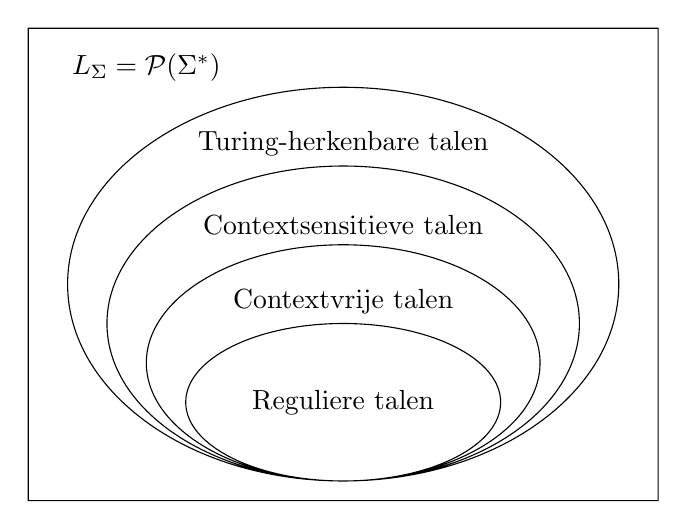
\begin{tikzpicture}
  \path
    (0,0) rectangle (8,6) [draw]
    (1.5,5.5) node {$L_\Sigma = \powerset(\sstar)$}
    (4,2.75) coordinate (A) node[above=1.5cm] {Turing-herkenbare talen} ellipse (3.5 and 2.5) [draw]
    (4,2.25) coordinate (B) node[above=1cm] {Contextsensitieve talen} ellipse (3 and 2) [draw]
    (4,1.75) coordinate (C) node[above=0.5cm] {Contextvrije talen} ellipse (2.5 and 1.5) [draw]
    (4,1.25) coordinate (D) node {Reguliere talen} ellipse (2 and 1) [draw];
  \end{tikzpicture}
  \caption{Een voorstelling van de Chomsky-hi\"erarchy.}
\end{figure}

\newpage\section{Turingmachines}

\begin{definitie}{Turingmachine}
  \label{def:tm}
  Een Turingmachine (TM) is een 7-tal ($Q$, $\Sigma$, $\Gamma$, $\delta$, $q_s$, $q_a$, $q_r$) waarbij
  \begin{itemize}
  \item $Q$ een eindige verzameling toestanden
  \item $\Sigma$ een eindig invoer alfabet dat $\#$ niet bevat
  \item $\Gamma$ een eindig tape alfabet met $\# \in \Gamma$ en $\Sigma \subset \Gamma$
  \item $q_s$ de starttoestand
  \item $q_a$ de accepterende eindtoestand
  \item $q_r$ de verwerpende eindtoestand verschillend van $Q_a$
  \item \bm{$\delta: Q \times \Gamma \rightarrow Q \times \Gamma \times \{L, R, S\}$}\\$\delta$ de (totale) transitiefunctie
  \end{itemize}
\end{definitie}

$\#$ wordt gebruikt om aan te geven dat een positie op de band van de TM nog niet beschreven is. We noemen dit het blanco symbool.

% TODO: Werking TM

\begin{definitie}{Opdeling van $\sstar$ door een TM}
  Een TM kan $\sstar$ in drie disjuncte stukken opdelen:
  \begin{itemize}
  \item $L_{TM}$: De taal met alle strings die door de TM worden geaccepteerd.
  \item $\infty_{TM}$: De taal met alle strings waarvoor de TM niet stopt.
  \item De resterende strings die door de TM worden verworpen.
  \end{itemize}
\end{definitie}

\begin{definitie}{(Turing-)herkenbaarheid}
  \vspace{-5mm}\begin{itemize}
  \item Een Turingmachine $TM$ herkent een taal $L_{TM}$.
  \item Een taal $L$ is herkenbaar indien er een Turingmachine $TM$ bestaat zodanig dat $L = L_{TM}$.
  \end{itemize}
\end{definitie}

\begin{definitie}{Co-herkenbaarheid}
  Een taal $L$ is co-herkenbaar indien $\overline{L}$ herkenbaar is.
\end{definitie}

\begin{definitie}{(Turing-)beslisbaarheid}
  \vspace{-5mm}\begin{itemize}
  \item Een Turingmachine $TM$ beslist een taal $L_{TM}$ indien $TM$ $L$ herkent en $\infty_{TM} = \emptyset$.
  \item Een taal $L$ is beslisbaar indien er een Turingmachine $TM$ bestaat zodanig die $L$ beslist.
  \item Een taal $L$ is beslisbaar indien ze herkenbaar en co-herkenbaar is.
  \end{itemize}
\end{definitie}

\begin{definitie}{Co-beslisbaarheid}
  Een taal $L$ die beslisbaar is is ook co-beslisbaar.
\end{definitie}

\begin{bewijs}{We bewijzen co-beslisbaarheid.}
  Als een beslisser $B$ de taal $L$ beslist, dan stopt die beslisser voor elke invoer bij de accepterende eindtoestand $q_a$ of de verwerpende eindtoestand $q_r$. We kunnen een beslisser $B'$ construeren voor $\overline{L}$ door bij $B$ de toestanden $q_a$ en $q_r$ om te wisselen. Omdat $B$ ook stopt voor alle strings die niet tot de taal behoren zal $B'$ die strings accepteren en alle strings die $B$ accepteert verwerpen. Bijgevolg is $\overline{L}$ beslisbaar.
\end{bewijs}

\begin{bewijs}{We bewijzen dat een taal beslisbaar is als ze herkenbaar en co-herkenbaar is.}
  Stel een machine $M_1$ herkent $L$ en een machine $M_2$ herkent $\overline{L}$. We construeren nu een machine $M$ die voor een string beide machines $M_1$ en $M_2$ laat lopen. Indien $M_1$ de string accepteert, dan accepteert $M$ de string. Indien $M_2$ de string accepteert, dan verwerpt $M$ de string. Omdat $M_1$ alle strings accepteert uit $L$ en $M_2$ alle strings uit $\overline{L}$, zal $M$ voor elke invoer stoppen in een eindtoestand. Bijgevolg is $M$ een beslisser voor $L$, dus is $L$ beslisbaar.
\end{bewijs}

Niet alle talen $L \in L_\Sigma$ zijn herkenbaar.
% TODO: Bewijs

% TODO: Grafische voorstelling Turingmachine
% TODO: Berekeningen van een TM voorstellen en nabootsen
% TODO: Deterministische Turinmachines
% TODO: Encodering

\begin{definitie}{Universele Turingmachine}
  \label{def:utm}
  Een universele Turingmachine (UTM) is een Turingmachine die andere TM's kan simuleren. Een UTM heeft een programmaband waar een encodering (transitietabel, $q_s$, $q_a$, $q_r$, ...) van een TM wordt ingegeven. Vervolgens wordt een inputstring $s$ ingegeven op een geheugenband. De UTM is vervolgens in staat om de originele TM te simuleren op basis van het ingegeven ``programma'' en dezelfde uitvoer te genereren.
\end{definitie}

\begin{definitie}{Het acceptatieprobleem voor TM's}
  Het acceptatieprobleem is de vraag of het mogelijk is om voor een gegeven Turingmachine $M$ en gegeven string $s$ te bepalen of $M$ $s$ accepteert.
  \begin{equation*}
  \atm = \{\langle M,s \rangle | M\text{ is een Turingmachine en }s \in L_M\}
  \end{equation*}
\end{definitie}

Er bestaat geen Turingmachine $B$ die kan beslissen of een gegeven Turingmachine $M$ een gegeven string $s$ accepteert. De taal $\atm$ is niet beslisbaar.

\begin{bewijs}{We bewijzen dat $\atm$ niet beslisbaar is.}
  We bewijzen dit door contradictie. Stel dat er een beslisser $B$ bestaat voor $\atm$. Bij een input $\langle M,s \rangle$ accepteert $B$ $M$ als $M$ $s$ accepteert en $B$ verwerpt $M$ als $M$ $S$ verwerpt of blijft lopen.

We construeren nu een contradictiemachine $C$ als
\begin{equation*}
C(\langle M \rangle) = opposite(B(\langle M,M \rangle))\text{ voor elke Turingmachine M}
\end{equation*}
De functie $opposite(x)$ is gedefinieerd als
\begin{equation*}
opposite(x) = \begin{cases}
reject, & \text{ als } x = accept\\
accept & \text{ als } x = reject
\end{cases}
\end{equation*}

We nemen nu $C(\langle C \rangle) = opposite(B(\langle C,C \rangle))$:
Als $C(\langle C \rangle) = accept$ ($C$ accepteert $C$), dan accepteert de beslisser $B$ de invoer $\langle C,C \rangle$, dus $B(\langle C,C \rangle) = accept$. Maar $opposite(B(\langle C,C \rangle))$ is dan $reject$, dat is een tegenstelling omdat dan geldt $C(\langle C \rangle) \neq opposite(B(\langle C,C \rangle))$.

We kunnen nu zeggen dat de machine $C$ niet kan bestaan, dus de beslisser $B$ kan ook niet bestaan. Bij gevolg is $\atm$ niet beslisbaar.
\end{bewijs}

\begin{definitie}{Het Halting-probleem voor TM's}
  \label{def:htm}
  Het Halting-probleem is de vraag of het mogelijk is om voor een gegeven Turingmachine $M$ en gegeven string $s$ te bepalen of $M$ stopt bij de invoer van $s$ m.a.w. dat $M$ $S$ accepteert of verwerpt.
  \begin{equation*}
  \htm = \{\langle M,s \rangle | M\text{ is een Turingmachine die stopt bij invoer }s \in L_M\}
  \end{equation*}
\end{definitie}

\begin{bewijs}{We bewijzen dat $\htm$ niet beslisbaar is.}
Stel dat $\htm$ beslisbaar is door een beslisser $H$. We construeren nu een beslisser $B$ voor $\atm$ als volgt:

Bij een invoer $\langle M,s \rangle$ laat $B$ de machine $H$ lopen op $\langle M,s \rangle$.
\begin{itemize}
\item Indien $H(\langle M,s \rangle) = accept$, dan stopt $M$ voor een invoer $s$ (dus $M(s) = accept$ of $M(s) = reject$). $B$ geeft als resultaat $M(s)$.
\item indien $H(\langle M,s \rangle) = reject$, dan stopt $M$ niet voor een invoer $s$. $B$ geeft als resultaat $reject$.
\end{itemize}
Omdat $\atm$ niet beslisbaar is, kan $B$ niet bestaan, dus kan ook $H$ niet bestaan. Bij gevolg is $\htm$ niet beslisbaar.

We zeggen dat $\atm$ reduceerbaar is naar $\htm$.
\end{bewijs}

\begin{bewijs}{We bewijzen dat $\atm$ herkenbaar is.}
  Het is mogelijk een herkenner $H$ voor $\atm$ te construeren die bij een invoer $\langle M,s \rangle$ $M$ laat lopen op $s$. $H$ accepteert de invoer $\langle M,s \rangle$ als $M$ de invoer $s$ accepteert en verwerpt de invoer als $M$ niet stopt bij invoer $s$ of $s$ verwerpt.
\end{bewijs}

\begin{bewijs}{We bewijzen dat $\htm$ herkenbaar is.}
  Het is mogelijk een herkenner $H$ voor $\htm$ te construeren die bij een invoer $\langle M,s \rangle$ $M$ laat lopen op $s$. $H$ accepteert de invoer $\langle M,s \rangle$ als $M$ stopt bij invoer $s$ en verwerpt de invoer als $M$ niet stopt bij invoer $s$.
\end{bewijs}

\begin{bewijs}{We bewijzen dat $\overline{\atm}$ niet herkenbaar is.}
  Stel dat $\overline{\atm}$ herkenbaar is en we weten dat $\atm$ herkenbaar is. Dan volgt dat $\atm$ beslisbaar is, wat niet mogelijk is. Bij gevolg kan $\overline{\atm}$ niet herkenbaar zijn. 
\end{bewijs}

\begin{bewijs}{We bewijzen dat $\overline{\htm}$ niet herkenbaar is.}
  Stel dat $\overline{\htm}$ herkenbaar is en we weten dat $\atm$ herkenbaar is. Dan volgt dat $\htm$ beslisbaar is, wat niet mogelijk is. Bij gevolg kan $\overline{\htm}$ niet herkenbaar zijn. 
\end{bewijs}

\subsection{Enumeratormachine}

\begin{definitie}{Enumeratormachine}
  Een enumeratormachine is een variant van een Turingmachine (definitie \ref{def:tm}) met een extra enumeratortoestand $q_e$ en een overgangsfunctie met als signatuur \bm{$\delta: Q \times \Gamma \rightarrow Q \times \Gamma \times \Gamma_\epsilon \times \{L, R, S\}$}. Bij een overgang wordt voor $\Gamma_\epsilon$ in de signatuur een teken op een outputband geschreven. Bij het bereiken van $q_e$ wordt een outputmarker op de outputband geschreven die een outputstring afscheidt van de volgende.
\end{definitie}

Een enumeratormachine produceert (enumereert) een verzameling strings op de outputband die de taal de taal vormt die door die machine bepaalt wordt. Een enumeratormachine stopt niet altijd of stopt niet altijd bij het uitschrijven van een individuele string.

\begin{bewijs}{We bewijzen dat een taal die door een enumerator bepaald wordt, herkenbaar is.}
  We construeren een herkenner $H$ voor de taal $L$ bepaald door een gegeven enumerator $Enu$. Bij de invoer van een string $s \in L$ laat $H$ $Enu$ lopen. Telkens $Enu$ de toestand $q_e$ bereikt, vergelijkt $H$ de gegeven string $s$ met de laatste string op de outputband. Als ze gelijk zijn, dan accepteert $H$ de taal, als ze niet gelijk zijn, laat het $Enu$ de volgende string genereren.
\end{bewijs}

\begin{bewijs}{We bewijzen dat elke herkenbare taal door een enumerator\\ge\"enumereerd wordt.}
    Het Halting-probleem geeft aan dat een Turingmachine niet noodzakelijk stopt voor elke string. Daarom construeren we een enumerator $Enu$ voor een herkenbare taal $L$ bepaald door $TM$ als volgt:
 
  We construeren
  \begin{itemize}
  \item een Turingmachine $TM_{gen}$ die gegeven een getal $n$, de $n$ eerste strings van $\sstar$ op de band zet.
  \item een Turingmachine $TM_n$ die gegeven een getal $N$, op elk van de $n$ strings, $n$ stappen van $TM$ uitvoert. Als $TM$ daarbij een string accepteert, dan wordt die weggeschreven op de outputband van $Enu$.
  \item een Turingmachine $TM_{driver}$ die opeenvolgende getallen $n$ genereert en vervolgens $TM_{gen}$ en $TM_n$ oproept.
  \end{itemize}
\end{bewijs}

\subsection{(Niet-)beslisbare talen}

\begin{bewijs}{We bewijzen dat $A_{DFA}$ beslisbaar is.}
  Voor $A_{DFA} = \{\langle D,s \rangle | D \text{ is een DFA en } D \text{ accepteert } s\}$ construeren we een beslisser $B$ als volgt:
 
  $B$ krijgt een input $\langle D,s \rangle$. $B$ simuleert de uitvoering van $D$ op $S$. Als $D$ $S$ accepteert, dan accepteert $B$ de invoer. Als $D$ $S$ verwerpt, dan verwerpt $B$ de invoer. Een DFA stopt altijd, dus is $B$ een beslisser voor $A_{DFA}$.
\end{bewijs}

\begin{bewijs}{We bewijzen dat $A_{NFA}$ beslisbaar is.}
  Voor $A_{NFA} = \{\langle N,s \rangle | N \text{ is een NFA en } N \text{ accepteert } s\}$ construeren we een beslisser $B$ als volgt:
 
 $B$ krijgt een input $\langle N,s \rangle$. De NFA $N$ wordt omgezet naar een DFA met algoritme \ref{alg:nfadfa}. Nu kunnen we een beslisser $B_D$ construeren voor die DFA en die laten lopen op $s$. $B$ geeft de uitvoer van $B_D$ terug.
\end{bewijs}

\begin{bewijs}{We bewijzen dat $A_{RegExp}$ beslisbaar is.}
  Voor $A_{RegExp} = \{\langle RE,s \rangle | RE \text{ is een reguliere expressie en } RE \text{ accepteert } s\}$ construeren we een beslisser $B$ als volgt:
 
 $B$ krijgt een input $\langle RE,s \rangle$. De reguliere expressie $RE$ wordt omgezet naar een NFA. Nu kunnen we een beslisser $B_N$ construeren voor die NFA en die laten lopen op $s$. $B$ geeft de uitvoer van $B_N$ terug.
\end{bewijs}

% TODO: E_DFA is beslisbaar
% TODO: EQ_DFA is beslisbaar
% TODO: A_CFG is beslisbaar

\begin{bewijs}{We bewijzen dat $E_{CFG}$ beslisbaar is.}
    We kunnen bewijzen dat $E_{CFG} = \{\langle G \rangle | G \text{ is een CFG en } L_G = \emptyset\}$ beslisbaar is door $G$ te transformeren als volgt:
  \begin{itemize}
  \item Voor een regel $A \rightarrow \alpha$ met $\alpha$ bestaande enkel uit terminals (inclusief $\epsilon$), dan:
  \begin{itemize}
  \item Verwijder alle producties waar $A$ aan de linkerkant staat.
  \item Vervang in elke regel waar $A$ rechts voorkomt, de voorkomens van $A$ door $\alpha$.
  \end{itemize}
  \item Herhaal de transformatie totdat:
  \begin{itemize}
  \item Het startsymbool verwijderd is, waarbij de invoer verworpen wordt, omdat dat betekent dat het mogelijk is een string af te leiden in het startsymbool.
  \item Er geen regels zijn van de benodigde vorm, waarbij de invoer aanvaard wordt, omdat de taal dan leeg is. (Het is dus niet mogelijk om een terminal te bereiken vanuit het startsymbool.)
  \end{itemize}
  \end{itemize}
  Door deze transformatie uit te voeren kunnen we voor elke CFG bepalen of die de lege taal bepaalt of niet en dus is $E_{CFG}$ beslisbaar.
  
  Merk op dat de grammatica getransformeerd wordt naar een niet-equivalente grammatica.
\end{bewijs}

\begin{bewijs}{We bewijzen dat $EQ_{CFG}$ niet beslisbaar is.}
    We kunnen bewijzen dat $EQ_{CFG} = \{\langle G_1,G_2 \rangle | G_1 \en G_2 \text{ zijn equivalente}$ $\text{CFG's}\}$ beslisbaar door $ALL_{CFG}$ te reduceren naar $EQ_{CFG}$.

  Stel dat $EQ_{CFG}$ beslisbaar is en $EQ$ is een beslisser voor $EQ_{CFG}$, dan kunnen we een beslisser $A$ voor $ALL_{CFG}$ construeren. Gegeven een invoer $\langle G \rangle$, laat $A$ $EQ$ lopen op $\langle G,G_1 \rangle$, waarbij $\langle G_1 \rangle$ een CFG is die de taal $\sstar$ genereert. $A$ geeft de uitvoer van $EQ$ terug. $A$ is nu een beslisser voor $ALL_{CFG}$, die niet kan bestaan, dus de beslisser $EQ$ voor $EQ_{CFG}$ kan ook niet bestaan.
\end{bewijs}

\begin{bewijs}{We bewijzen dat $ES_{CFG}$ beslisbaar is.}
  We kunnen bewijzen dat $ES_{CFG} = \{\langle G \rangle | G \text{ is een CFG en } \epsilon \in L_G\}$ beslisbaar is door $G$ te transformeren naar de Chomsky Normaal Vorm (definitie\ref{def:cnf}). Indien de CNF de productie ``$S \rightarrow \epsilon$'' bevat kunnen we concluderen dat de gegeven CFG $G$ de lege string bevat. Bij gevolg is $ES_{CFG}$ beslisbaar.
\end{bewijs}

% TODO: Elke CFL is beslisbaar
% TODO: A_LBA is beslisbaar
% TODO: E_LBA is beslisbaar

\begin{bewijs}{We bewijzen dat $\etm$ niet beslisbaar is.}
    Stel dat $\etm$ beslisbaar is en $E$ is een beslisser voor $\etm$, dan kunnen we een beslisser $B$ voor $\atm$ construeren. Voor een gegeven invoer $\langle M,s \rangle$ construeren we een machine $M_s$ waarvoor geldt
  \begin{itemize}
  \item Gegeven een invoer $w$, als $w \neq s$, verwerpt $M_s$ de string $w$.
  \item Anders laat $M_s$ $M$ lopen op $w$ en geeft hetzelfde resultaat terug.
  \end{itemize}
  $M_s$ is een machine die enkel accept teruggeeft indien $M$ $s$ accepteert en anders reject. We laten $E$ lopen op $\langle M_s \rangle$:
  \begin{itemize}
  \item Als $E$ $M_s$ accepteert, dan laten we $B$ zijn input $\langle M,s \rangle$ verwerpen, omdat $M_s$ dan de lege taal bepaalt, wat enkel mogelijk is als $M$ $s$ verwerpt.
  \item Als $E$ $M_s$ verwerpt, dan laten we $B$ zijn input $\langle M,s \rangle$ accepteren, omdat $M_s$ dan niet de lege taal bepaalt, wat enkel mogelijk is als $M$ $s$ accepteert.
  \end{itemize}
  
  We zeggen dat $\overline{\atm}$ reduceerbaar is naar $\etm$.
\end{bewijs}

\begin{bewijs}{We bewijzen dat $\eqtm$ niet beslisbaar is.}
  We kunnen $\etm$ reduceren naar $\eqtm$ ($\etm \leq_m \eqtm$). Indien er een beslisser $EQ$ bestaat voor $\eqtm$, dan kunnen we een beslisser $E$ voor $\etm$ bouwen die bij een invoer $\langle M \rangle$, $EQ$ laat lopen op $\langle M,M_\emptyset \rangle$ en hetzelfde resultaat teruggeeft. We weten dat $\etm$ niet beslisbaar is, dus de beslisser $E$ kan niet bestaan en dus de beslisser $EQ$ ook niet. Bijgevolg is $\eqtm$ ook niet beslisbaar.
\end{bewijs}

% TODO: EQ_TM is niet (co-)herkenbaar

\begin{definitie}{$IsIn_{TM,S}$}
  Stel dat $S$ een verzameling van talen is, kunnen we voor een gegeven machine $M$ bepalen of de taal $L_M$ bepaald van die machine behoort tot de verzameling $S$?
  \begin{equation*}
  IsIn_{TM,S} = \{\langle M \rangle|L_M \in S\}
  \end{equation*}
\end{definitie}

We kunnen zeggen dat $\etm = IsIn_{TM,\{\emptyset\}}$ en $REGULAR_{TM} = IsIn_{TM,RegLan}$.

% TODO: REGULAR_TM is niet beslisbaar: $REGULAR_{TM} = \{\langle M \rangle | M \text{ is een Turingmachine en } L_M \text{ is een reguliere taal}\}$

\subsubsection{Overzicht}
De onderstaande tabel geeft voor heel wat talen weer of ze herkenbaar (H), co-herkenbaar (cH) en beslisbaar (B) zijn:

\LTXtable{\textwidth}{tabelbeslisbaar.tex}

% TODO: Aftelbaarheid

\subsection{Stelling van Rice}

Een eigenschap $P$ van Turingmachines verdeelt die in twee verzamelingen. De machines met die eigenschap $Pos_P = \{M|P(M)=true\}$ en de machines zonder die eigenschap $Neg_P = \{M|P(M)=false\}$. Samen vormen ze een partitie $\{Pos_P, Neg_P\}$ van de verzameling van alle Turingmachines.

\begin{definitie}{Niet-triviale eigenschap}
    Een eigenschap $P$ is niet triviaal indien $Pos_P \neq \emptyset$ en $Neg_P \neq \emptyset$.
\end{definitie}

\begin{definitie}{Taal-invariante eigenschap}
    Een eigenschap $P$ is taal-invariant als alle machines die dezelfde taal bepalen ook die eigenschap gemeenschappelijk hebben (of geen enkel van die machines die eigenschap heeft).
  \begin{equation*}
  L_{M_1} = L_{M_2} \Rightarrow P(M_1) = P(M_2)
  \end{equation*}
\end{definitie}

\begin{definitie}{Eerste stelling van Rice}
    Voor elke niet-triviale, taal-invariante eigenschap $P$ van Turingmachines geldt dat $Pos_P$ niet beslisbaar is. (Ook $Neg_P$ is niet beslisbaar, maar dat volgt uit $Neg_P = \overline{Pos_P}$.)
\end{definitie}

\begin{bewijs}{We bewijzen de eerste stelling van Rice}
    Stel dat $M_\emptyset$ die de lege taal bepaalt, een eigenschap $P$ niet heeft. Omdat $P$ niet-triviaal is, moet er een machine $X$ bestaat die de taal $L_X$ bepaalt en de eigenschap $P$ wel heeft.

  Stel dat er een beslisser $B$ bestaan voor $Pos_P$, dan kunnen we een beslisser $A$ voor $A_{TM}$ construeren. Voor een gegeven invoer $\langle M,s \rangle$ construeren we een hulpmachine $H_{M,s}$ waarvoor geldt
  \begin{itemize}
  \item $H_{M,s}$ laat $M$ lopen op $s$.
  \item Als $M$ $s$ accepteert, dan laat $H_{M,s}$ $X$ lopen op een invoer $x$ en accepteert indien $X$ $x$ accepteert.
  \end{itemize}
  
  We kunnen zeggen dat voor $H_{M,s}$ geldt dat het de taal $L_X$ bepaalt indien $M$ $s$ accepteert en de lege taal bepaalt indien $M$ $s$ niet accepteert. Dat wilt zeggen dat $H_{M,s}$ de eigenschap $P$ heeft indien $M$ $s$ accepteert en de eigenschap $P$ niet heeft indien $M$ $s$ niet accepteert.
  
  Bijgevolg kunnen we zeggen dat $A$ een invoer $\langle M,s \rangle$ accepteert als $B$ $H_{M,s}$ accepteert en de invoer verwerpt als $B$ $H_{M,s}$ verwerpt. Dus $A$ is een beslisser voor $\atm$, wat niet mogelijk is. Daarom kan de beslisser $B$ voor $Pos_P$ ook niet bestaan.
  
  We zeggen dat $\atm$ reduceerbaar is naar $Pos_P$.
  
  Als $M_\emptyset$ de eigenschap $P$ wel heeft, kunnen we het bewijs uitvoeren voor $\overline{P}$. Omdat we dan bewijzen dat $Pos_{\overline{P}} = Neg_P$ onbeslisbaar is, weten we dat ook $Pos_P = \overline{Neg_P}$ onbeslisbaar is.
\end{bewijs}

% TODO: Tweede stelling van Rice?
% TODO: Post Correspondence Problem

\subsection{Reductie}

\begin{definitie}{Turing-berekenbare functie}
  Een functie $f$ is Turing-berkenbaar als er een Turingmachine bestaat die bij een invoer van $s$, stopt met $f(s)$ op de band.
\end{definitie}

\begin{definitie}{Reductie van talen}
  Een taal $L_1$ over $\Sigma_1$ kan gereduceerd worden naar een taal $L_2$ over $\Sigma_2$ als er een afbeelding \bm{$f: \sstar_1 \rightarrow \sstar_2$} bestaat zodanig dat $f(L_1) \subseteq L_2$ en $f(\overline{L_1}) \subseteq \overline{L_2}$ met $f$ een Turing-berkenbare functie.
  \begin{equation*}
  L_1 \leq_m L_2
  \end{equation*}
\end{definitie}

\begin{itemize}
\item Als $L_1 \leq_m L_2$ en $L_1$ is niet beslisbaar, dan is $L_2$ niet beslisbaar.
\item Als $L_1 \leq_m L_2$ en $L_2$ is beslisbaar, dan is $L_1$ beslisbaar.
\item Als $L_1 \leq_m L_2$ en $L_1$ is niet herkenbaar, dan is $L_2$ niet herkenbaar.
\item Als $L_1 \leq_m L_2$ en $L_2$ is herkenbaar, dan is $L_1$ herkenbaar.
\end{itemize}

We kunnen bewijzen dat $\eqtm$ niet beslisbaar is met de functie $f$ die $E(\langle M \rangle)$ afbeeldt op $EQ(\langle M,M_\emptyset \rangle)$. We noteren $\etm \leq_m \eqtm$.

% TODO: Bewijs dat als L1 naar L2 reduceert, dat \overline{L1} ook naar \overline{L2} reduceert.
% TODO: Bewijs EQ_TM is net herkenbaar en niet co-herkenbaar

\subsection{Orakelmachines}

\begin{definitie}{Orakelmachine}
  Een orakelmachine is een Turingmachine die vragen kan stellen aan een orakel over een taal/probleem. Het orakel kan in een eindig (klein) aantal stappen een antwoord teruggeven aan de orakelmachine.
\end{definitie}

We kunnen een orakelmachine $\oatm$ bouwen die $\atm$ beslist. De verzameling van orakelmachines met $\oatm$ is strikt sterker van de verzameling van de Turingmachines omdat die meer talen beslist/herkent. Aangezien dat heel wat talen niet beslisbaar (of zelfs herkenbaar) zijn omdat $\atm$ niet beslisbaar is.

\begin{bewijs}{We bewijzen dat er een $\oatm$ bestaat die $\etm$ beslist.}
    We construeren een Orakelmachine $\oatm$. Bij input $\langle M \rangle$ doet $\oatm$:
  \begin{itemize}
  \item Construeer een Turingmachine $P$ die bij input $w$:
  \begin{itemize}
  \item $M$ laat lopen op alle strings van $\sstar$.
  \item Als $M$ eender welke string van $\sstar$ accepteert, dan accepteert $P$ de input $w$. ($P$ accepteert voor eendere welke $w$ zo lang dat $M$ minstens \'e\'en string accepteert en dus niet de lege taal bepaalt.)
  \end{itemize}
  \item $\oatm$ vraagt aan het orakel of $\langle P,w \rangle \in \atm$.
  \item Als het orakel ``ja'' antwoordt, dan verwerpt $\oatm$ de invoer, omdat $M$ niet de lege taal bepaalt. Anders accepteert het de invoer.
  \end{itemize}
  
  $\oatm$ is een beslisser voor de taal $\etm$.
\end{bewijs}

\begin{definitie}{Turingreduceerbaarheid}
  Een taal $A$ is Turingeduceerbaar naar een taal $B$ indien er een orakelmachine $O^B$ bestaat die $A$ beslist. We zeggen dat $A$ beslisbaar is t.o.v. $B$.
  \begin{equation*}
  A \leq_T B
  \end{equation*}
\end{definitie}

\begin{itemize}
\item Indien $A \leq_T B$ en $B$ is beslisbaar, dan is $A$ beslisbaar.
\item $\leq_m$ is fijner dan $\leq_T$, dus $A \leq_m B \rightarrow A \leq_T B$
\end{itemize}

De taal $\{O|O\text{ is een orakelmachine met een orakel voor }\atm\}$ kan niet elke taal beslissen want die verzameling is aftelbaar en de verzameling van alle talen $\l_\Sigma$ is niet-aftelbaar. Dus er bestaat minstens \'e\'en taal X die niet beslisbaar is met de hulp van een orakel voor $\atm$.

% TODO: Turingberekenbare functies!!
% TODO: Bezige bever en stijgende functies

\newpage\section{Lambda calculus}

$\lambda$-calculus is een herschijfsysteem dat de basis vormt voor functionele programmeertalen zoals Haskell.

\begin{definitie}{$\lambda$-expressie}
  Een $\lambda$-expressie $<exp>$ kan \'e\'en van de volgende vormen aannemen:
  \begin{itemize}
  \item $<const>$: Een constante.
  \item $<var>$: Een variabele.
  \item $<exp> <exp>$: De toepassing van een functie op een argument.
  \item $\lambda<var>. <exp>$: Een $\lambda$-abstractie die een variabele bindt.
  \item $(<exp>)$: Een expressie omsloten door haakjes.
  \end{itemize}
\end{definitie}

\begin{definitie}{Currying}
  Het toepassen van een functie in een $\lambda$-expressie kan steeds maar op \'e\'en argument. Currying is een techniek die wordt toegepast om een functie te herschrijven naar een opeenvolging van functietoepassingen op telkens \'e\'en element.
\end{definitie}

Een simpel voorbeeld van currying is de functie $+$ voor natuurlijke getallen:\\
\bm{$+: \nat \times \nat \rightarrow \nat$}\\
$(+\ a\ b)$

Deze functie wordt d.m.v. currying vertaalt naar:\\
\bm{$+: \nat \rightarrow (\nat \rightarrow \nat)$}\\
$((+\ a)\ b)$

Bij bovenstaande functie is $(+\ a)$ een functie die een getal $i$ afbeeldt op $a + i$.

\begin{definitie}{Deel-expressie}
  Een deel-expressie van een $\lambda$-expressie is een geneste $\lambda$-expressie.
\end{definitie}

\begin{definitie}{Redex}
  Een deel-expressie van een $\lambda$-expressie is een redex indien zijn parameters getallen zijn en de expressie reduceerbaar is.
\end{definitie}

\begin{definitie}{Reductie}
  Een reductie is het reduceren van de redex in een $\lambda$-expressie door meestal een functie evaluatie uit te voeren. Gewoonlijk wordt de meest linkse redex eerst gereduceerd.
\end{definitie}

\begin{definitie}{Normaalvorm}
  Een $\lambda$-expressie in normaalvorm is een expressie die geen redex bevat. Niet elke $\lambda$-expressie heeft een normaalvorm. Indien er een equivalente normaalvorm bestaat voor een expressie, dan bestaat er een rij reductieregels die die expressie omvormen tot de normaalvorm.
\end{definitie}

\begin{definitie}{$\lambda$-abstractie}
  Een $\lambda$-abstractie is een functie definitie van de vorm:
  \begin{itemize}
  \item $\lambda$
  \item $<var>$: \'E\'en variabele.
  \item $.$: Dit punt scheidt de definitie van de variabele van het lichaam van de functie.
  \item $<exp>$: De expressie die aangeeft hoe de functie moet berekent worden.
  \end{itemize}
\end{definitie}

Een alternatieve notatie voor een $\lambda$-expressie met twee (of meerdere) variabelen bestaat ook. Een voorbeeld: $(\lambda x\ y.(+\ x\ y)) = (\lambda x.(\lambda y.(+\ x\ y)))$

\begin{definitie}{Vrije/gebonden variabele}
  Een variabele in een $\lambda$-expressie is gebonden indien die expressie genest is in een $\lambda$-abstractie die de variabele met die naam definieert. Een variabele die vrij is, is niet gedefinieerd. We zeggen dat een variabele $x$ vrij is in een expressie $E$ indien:
  \begin{itemize}
  \item $E == x$
  \item $E == (A\ B)$ en er is een vrij voorkomen van $x$ in $A$ of $B$.
  \item $E == (\lambda y. A)$ en $x \neq y$ en er is een vrij voorkomen van $x$ in $A$
  \end{itemize}
\end{definitie}

Een variabele gedefinieerd in een $\lambda$-abstractie wordt gebonden aan alle vrije voorkomens van die variabele in de deelexpressie (en verder geneste deelexpressies) van die $\lambda$-abstractie.

\subsection{Herschrijfregels van lambda calculus}

Elke conversie regel is een samenstelling van een reductieregel ($\longrightarrow$) en een abstractieregel ($\longleftarrow$) die een equivalentie beschrijft. Een abstractie is de inverse operatie van een reductie. Twee expressies $A$ en $B$ zij equivalent onder een rij conversie als $\stackrel{*}{\longleftrightarrow}$. Indien er een rij reducties bestaat die $A$ naar $B$ reduceert, schrijven we $\stackrel{*}{\longrightarrow}$.

\begin{definitie}{$\beta$-reductie}
  $\beta$-reductie ($\stackrel{\beta}{\longrightarrow}$) is een syntactische herschrijfregel die een $\lambda$-abstractie herschrijft naar het lichaam van die $\lambda$-abstractie met de formele parameter vervangen door het argument. Deze reductie wordt gebruikt bij een functietoepassing.
\end{definitie}

Een voorbeeld van $\beta$-reductie: $(\lambda x.\ +\ x\ x)\ 5 \stackrel{\beta}{\longrightarrow} +\ 5\ 5$.

\begin{definitie}{$\beta$-abstractie}
  $\beta$-abstractie ($\stackrel{\beta}{\longleftarrow}$) is een syntactische herschrijfregel die de inverse operatie van een $\beta$-reductie uitvoert door een expressie in een $\lambda$-abstractie te plaatsen en \'e\'en (of meerdere gelijke) deelexpressies te vervangen door de formele parameter, zodanig dat de expressie een argument wordt.
\end{definitie}

Een voorbeeld van $\beta$-abstractie: $+\ 5\ 5 \stackrel{\beta}{\longrightarrow} (\lambda x.\ +\ x\ x)\ 5$.

\begin{definitie}{$\alpha$-reductie of $\alpha$-abstractie}
  $\alpha$-reductie ($\stackrel{\alpha}{\longrightarrow}$) is een herschrijfregel (hernoemingsregel) die alle vrije voorkomens van de formele parameter in het lichaam van een $\lambda$-abstractie hernoemt. De $\alpha$-abstractie operatie is identiek aan $\alpha$-reductie ($\stackrel{\alpha}{\longleftarrow}$), dus kunnen voor beiden de term $\alpha$-conversie ($\stackrel{\alpha}{\longleftrightarrow}$) gebruiken.
\end{definitie}

Een voorbeeld van $\alpha$-conversie: $(\lambda x.\ +\ x\ x) \stackrel{\alpha}{\longleftrightarrow} (\lambda y.\ +\ y\ y)$.

\begin{definitie}{$\eta$-reductie of $\eta$-abstractie}
  $\eta$-reductie ($\stackrel{\eta}{\longrightarrow}$) is een herschrijfregel die een functietoepassing waaraan een $\lambda$-abstractie slechts een parameter doorgeeft herschrijft naar zijn equivalent zonder de $\lambda$-abstractie. De $\eta$-abstractie operatie is de inverse van $\eta$-reductie ($\stackrel{\eta}{\longleftarrow}$). We spreken over een regel die equivalentie aantoont dus wordt meestal $\eta$-conversie ($\stackrel{\eta}{\longleftrightarrow}$) gebruikt.
\end{definitie}

Een voorbeeld van $\eta$-conversie: $(\lambda x.\ F\ x) \stackrel{\eta}{\longleftrightarrow} F$.

% TODO: Name capture problem

\begin{definitie}{$\delta$-reductie of $\delta$-abstractie}
  $\delta$-reductie ($\stackrel{\delta}{\longrightarrow}$) is een herschrijfregel die functies intern aan de taal toepast op een argument in de expressie. De $\delta$-abstractie operatie is de inverse van $\delta$-reductie die een expressie vervangt door een expressie en een interne operatie die samen equivalent zijn aan de originele expressie.
\end{definitie}

Een voorbeeld van $\delta$-conversie: $+\ 5\ 5 \stackrel{\delta}{\longleftrightarrow} 10$.

% TODO: Church numerals

\begin{definitie}{Oneindige lus}
  Een oneindige lus is een expressie die nooit in normaalvorm kan gebracht worden. Een oneindige lus kan zeer makkelijk gemodelleerd worden als $(\lambda x. x\ x)(\lambda x. x\ x)$ omdat bij elke reductie terug dezelfde expressie verkregen wordt.
\end{definitie}

\subsection{Reductie in normaalorde}

\begin{definitie}{Church-Rosser I (CR1)}
    Church-Rosser I verwijst naar de eerste stelling van Church en Rosser. Die stelling zegt dat indien $E_1 \stackrel{*}{\longleftrightarrow} E_2$ geldt, dat er een expressie $E$ moet bestaan in normaalvorm zodanig dat $E_1 \stackrel{*}{\longrightarrow} E$ en $E_2 \stackrel{*}{\longrightarrow} E$.
\end{definitie}

\begin{bewijs}{We bewijzen de uniciteit van de normaalvorm.}
  Stel dat $E \stackrel{*}{\longleftrightarrow} E_1$ en $E \stackrel{*}{\longleftrightarrow} E_2$ gelden, waarbij dat $E_1$ en $E_2$ in normaalvorm staan. Dan moet gelden dat $E_1 \stackrel{*}{\longleftrightarrow} E_2$. Volgend CR1 moet dan gelden dat er een normaalvorm $F$ bestaat zodanig dat $E_1 \stackrel{*}{\longleftrightarrow} F$ en $E_2 \stackrel{*}{\longleftrightarrow} F$. Omdat $E_1$ en $E_2$ reeds in normaalvorm staan, zijn er in geen van beiden expressies nog redexen die gereduceerd kunnen worden, dus concluderen we dat (eventueel onder $\alpha$-conversie) $E_1 = F = E_2$.
\end{bewijs}

\begin{definitie}{Reductie in normaalorde}
Bij reductie in normaalorde wordt steeds de meest linkse buitenste redex eerst gereduceerd.
\end{definitie}

Reductie in normaalorde garandeert dat een normaalvorm gevonden wordt (indien mogelijk), maar is niet noodzakelijk optimaal. Het is mogelijk dat een andere reductieorde een reductierij oplevert met minder stappen. Een voorbeeld daarvan is de ``call-by-value'' techniek, waarbij eerst een argument voor een functie wordt gereduceerd. Een expressie die wordt doorgegeven als argument voor reductie, kan mogelijk meerdere keren ge\"evalueerd worden.

\begin{definitie}{Church-Rosser II (CR2)}
    Church-Rosser II verwijst naar de tweede stelling van Church en Rosser. Die stelling zegt dat indien $E \stackrel{*}{\longleftrightarrow} N$  bestaat met $N$ in normaalvorm, dat er een reductierij moet bestaan in normaalorde van $E$ naar $N$.
\end{definitie}

\begin{definitie}{Turing-compleetheid}
  \label{def:tmcompleet}
  Een systeem is Turing-compleet indien het elke Turing-berekenbare functie kan voorstellen. Zulk systeem kan ook een Universele Turingmachine (definitie \ref{def:utm}) simuleren.
\end{definitie}

\begin{definitie}{Turing-equivalentie}
  Een systeem is Turing-equivalent indien het Turing-compleet is (definitie \ref{def:tmcompleet}) en indien het kan gesimuleerd worden door een Universele Turingmachine (definitie \ref{def:utm}).
\end{definitie}

\begin{definitie}{Turing-equivalente $\lambda$-calculus}
  \label{def:tmlambda}
  $\lambda$-calculus is Turing-equivalent omdat het alle Turing-berekenbare functies voorstellen kan voorstellen en bovendien de verzameling van functies die het kan voorstellen even sterk is als die van Turingmachines. Turing-compleetheid van $\lambda$-calculus volgt intu\"itief uit de volgende eigenschappen:
  \begin{itemize}
  \item De reductie naar normaalvorm van een expressie heeft steeds slechts \'e\'en resultaat als die reductie een eindig aantal stappen heeft, namelijk de redex, ongeacht de reductieorde. We weten dat een Turingmachine slechts \'e\'en taal bepaalt.
  \item Wanneer een expressie niet naar normaalvorm gereduceerd kan worden, is er een lus waardoor de reductie nooit eindigt. Het Halting-probleem (definitie \ref{def:htm}) bestaat dus ook voor $\lambda$-calculus, net zoals ook de uitvoering van een Turingmachine stopt niet altijd.
  \end{itemize}
\end{definitie}

Intu\"itief is het makkelijk voor te stellen dat er voor elke Turingmachine die een taal $L_{TM}$ bepaalt een Turing-berekenbare functie bestaat die voor elke string $s \in L_{TM}$, $accept$ als uitvoer geeft en voor elke string $s \in \overline{L_{TM}}$, $reject$ als uitvoer geeft. Omdat $\lambda$-calculus Turing-compleet is moet er een $\lambda$-expressie bestaan die hetzelfde doet. Omgekeerd is het ook logisch dat er een Turing-berekenbare functie bestaat die een $\lambda$-expressie kan afbeelden op zijn normaalvorm.

\subsection{Recursieve functies}

Indien een $\lambda$-calculus toelaat om functies bij naam te defini\"eren of naar zichzelf te laten verwijzen, is het mogelijk om recursieve functies op te stellen. Dat is echter ook mogelijk in pure $\lambda$-calculus met een vastpuntcombinator.

\begin{definitie}{Vastpuntcombinator}
  Een vastpuntcombinator (FPC) is een functie $Y$ die voldoet aan
  \begin{equation*}
  \forall F: Y\ F = F\ (Y\ F)
  \end{equation*}
  De vastpuntcombinator van Curry wordt veel gebruikt en is gedefinieerd als
  \begin{equation*}
  \lambda f.\ (\lambda x.\ f\ (x\ x))\ (\lambda x.\ f\ (x\ x))
  \end{equation*}
\end{definitie}

Sectie \ref{ex:lambdarecurse} toont een voorbeeld van een recursieve functie ge\"mplementeerd in zuivere $\lambda$-calculus en de uitvoering ervan.

% TODO: Programmeertalen

\section{Voorbeelden}

\subsection{NFA $\longrightarrow$ RE}
\label{ex:gnfa}

\begin{nfa}
  \node[state]           (S)                    {$S$};
  \node[state]           (A) [below right of=S] {$A$};
  \node[state,accepting] (E) [above right of=A] {$E$};
  
  \path (S) edge []           node         {$a$}          (E)
            edge []           node         {$a,\epsilon$} (A)
        (A) edge [loop below] node         {$b$}          (A)
            edge [bend right] node         {$a$}          (E)
        (E) edge [loop right] node         {$a,b$}        (E)
            edge [bend right] node [above] {$\epsilon$}   (A);
  \addvmargin{1mm}
\end{nfa}

\paragraph{Stap 1} Generaliseren

\begin{nfa}
  \node[initial,state]   (SN)                    {$q_s$};
  \node[state]           (S)  [right of=SN]      {$S$};
  \node[state]           (A)  [below right of=S] {$A$};
  \node[state]           (E)  [above right of=A] {$E$};
  \node[state,accepting] (EN) [right of=E]       {$q_e$};
  
  \path (SN) edge []           node         {$\epsilon$}   (S)
        (S)  edge []           node         {$a$}          (E)
             edge []           node         {$a|\epsilon$} (A)
        (A)  edge [loop below] node         {$b$}          (A)
             edge [bend right] node         {$a$}          (E)
        (E)  edge [loop above] node         {$a|b$}        (E)
             edge [bend right] node [above] {$\epsilon$}   (A)
             edge []           node         {$\epsilon$}   (EN);
  \addvmargin{1mm}
\end{nfa}

\paragraph{Stap 2} Reductie (met vereenvoudiging)

Reductie 1:\\
\begin{nfa}
  \node[initial,state]   (SN)                    {$q_s$};
  \node[state]           (S)  [right of=SN]      {$S$};
  \node[state]           (A)  [below right of=S] {$A$};
  \node[state]           (E)  [above right of=A] {$E$};
  \node[state,accepting] (EN) [right of=E]       {$q_e$};
  
  \path (SN) edge []           node {$\epsilon$}   (S)
        (S)  edge []           node {$a$}          (E)
             edge []           node {$a|\epsilon$} (A)
        (A)  edge [loop below] node {$b$}          (A)
             edge []           node {$a$}          (E)
        (E)  edge [loop above] node {$a|b|b^*a$}   (E)
             edge []           node {$\epsilon$}   (EN);
  \addvmargin{1mm}
\end{nfa}

\begin{nfa}
  \node[initial,state]   (SN)                  {$q_s$};
  \node[state]           (S)  [right of=SN]    {$S$};
  \node[state]           (E)  [right=2cm of S] {$E$};
  \node[state,accepting] (EN) [right of=E]     {$q_e$};
  
  \path (SN) edge []           node {$\epsilon$}         (S)
        (S)  edge [bend right] node {$(a|\epsilon)b^*a$} (E)
             edge [bend left]  node {$a$}                (E)
        (E)  edge [loop above] node {$b|b^*a$}           (E)
             edge []           node {$\epsilon$}         (EN);
  \addvmargin{1mm}
\end{nfa}

\begin{nfa}
  \node[initial,state]   (SN)                  {$q_s$};
  \node[state]           (S)  [right of=SN]    {$S$};
  \node[state]           (E)  [right=3cm of S] {$E$};
  \node[state,accepting] (EN) [right of=E]     {$q_e$};
  
  \path (SN) edge []           node {$\epsilon$}         (S)
        (S)  edge []           node {$(a|\epsilon)b^*a$} (E)
        (E)  edge [loop above] node {$b|b^*a$}              (E)
             edge []           node {$\epsilon$}         (EN);
  \addvmargin{1mm}
\end{nfa}

Reductie 2:\\
\begin{nfa}
  \node[initial,state]   (SN)                  {$q_s$};
  \node[state]           (S)  [right of=SN]    {$S$};
  \node[state,accepting] (EN) [right=4cm of S] {$q_e$};
  
  \path (SN) edge [] node {$\epsilon$}                   (S)
        (S)  edge [] node {$(a|\epsilon)b^*a(b|b^*a)^*$} (EN);
  \addvmargin{1mm}
\end{nfa}

\begin{nfa}
  \node[initial,state]   (SN)                  {$q_s$};
  \node[state]           (S)  [right of=SN]    {$S$};
  \node[state,accepting] (EN) [right=4cm of S] {$q_e$};
  
  \path (SN) edge [] node {$\epsilon$}                   (S)
        (S)  edge [] node {$(a|\epsilon)b^*a(a|b)^*$} (EN);
  \addvmargin{1mm}
\end{nfa}

Reductie 3:\\
\begin{nfa}
  \node[initial,state]   (SN)                   {$q_s$};
  \node[state,accepting] (EN) [right=4cm of SN] {$q_e$};
  
  \path (SN) edge [] node {$(a|\epsilon)b^*a(a|b)^*$} (EN);
  \addvmargin{1mm}
\end{nfa}

\begin{nfa}
  \node[initial,state]   (SN)                   {$q_s$};
  \node[state,accepting] (EN) [right=4cm of SN] {$q_e$};
  
  \path (SN) edge [] node {$b^*a(a|b)^*$} (EN);
  \addvmargin{1mm}
\end{nfa}

\paragraph{Stap 3} De RE voor de NFA is ``$b^*a(a|b)^*$".
\section{Examenvragen}

\subsection{Reguliere talen}

\subsubsection{Vraag 1 - GNFA}

\textit{Bewijs dat een reguliere taal beschreven door een reguliere expressie door een eindige toestandsautomaat wordt herkend. Doe dit door van de automaat een gegeneraliseerde niet-deterministische eindige toestandsautomaat te maken. Beschrijf in detail hoe uit die GNFA een reguliere expressie kan worden afgeleid.}

\paragraph{Algoritme om de omzetting uit te voeren.}
\begin{enumalgo}
  \item Generaliseer de NFA:
    \begin{itemize}
    \item Voer een nieuwe begintoestand $q_s$ in.
    \item Voer een nieuwe (unieke) eindtoestand $q_e$ in.
    \item Teken $\epsilon$-boog van $q_s$ naar de oude begintoestand.
    \item Teken $\epsilon$-boog van elke oude eindtoestand naar $q_e$.
    \item Vul de automaat aan met $\phi$-bogen waar er bogen ontbreken. (Zie definitie \ref{def:gnfa})
    \item Neem parallelle gerichte bogen samen met de unie van hun labels.
    \end{itemize}
  \item Reduceer de GNFA:
    \begin{itemize}
    \item Als $Q \setminus \{q_s, q_e\} = \emptyset$, ga naar stap 3.
    \item Voer een reductiestap uit door een willekeurige toestand $q \in Q \setminus \{q_s, q_e\}$ te verwijderen. De basis reductiestap:\\
    \begin{tabular}{>{\centering\arraybackslash}m{3.5cm}>{\centering\arraybackslash}m{1cm} >{\centering\arraybackslash}m{4cm}}
\begin{nfa}
  \node[state] (A)                     {$q_a$};
  \node[state] (X)  [below right of=A] {$q$};
  \node[state] (B)  [above right of=X] {$q_b$};
  
  \path (A) edge [bend left]  node {$E_4$} (B)
            edge [bend right] node {$E_1$} (X)
        (X) edge [loop below] node {$E_2$} (X)
            edge [bend right] node {$E_3$} (B);
  \addvmargin{1mm}
\end{nfa} & $\longrightarrow$ & \begin{nfa}
  \node[state] (A)                   {$q_a$};
  \node[state] (B)  [right=2.5cm of A] {$q_b$};
  
  \path (A) edge []  node {$E_4|E_1(E_2)^*E_3$} (B);
  \addvmargin{1mm}
\end{nfa}
\end{tabular}
    \item Herhaal stap 2.
    \end{itemize}
  \item Bepaal de reguliere expressie die af te lezen is als label op de boog tussen $q_s$ en $q_e$.
  \end{enumalgo}
  
\paragraph{Bewijs.}   We bewijzen dit door aan te tonen dat een NFA kan omgezet worden naar een reguliere expressie die dezelfde taal bepaalt. Daarom tonen we aan dat bij algoritme \ref{alg:nfagnfa} de verzameling van aanvaarde strings in elke stap niet verandert.
  
  We kunnen een pad om een string te accepteren doorheen toestanden van een GNFA beschrijven als $E_1E_2E_3...E_n$ met $n$ het aantal toestanden om de eindtoestand te bereiken en $E_i$ reguliere expressies. We verwijzen naar de GNFA voor een reductiestap met $GNFA_{voor}$ en erna met $GNFA_{na}$.
  \begin{enumalgo}
  \item De omzetting van NFA naar GNFA wijzigt de verzameling aanvaarde strings niet:
  \begin{itemize}
  \item Stel dat NFA dezelfde taal $L_E$ bepaalt als een reguliere expressie $E$. Een nieuwe begintoestand toevoegen met een $\epsilon$ boog naar de oude staat gelijk aan de expressie $\epsilon E$, dewelke gelijk is aan $E$.
  \item Stel dat NFA dezelfde taal $L_E$ bepaalt als een reguliere expressie $E$. Een nieuwe eindtoestand toevoegen met een $\epsilon$ bogen van de oude toestanden naar de nieuwe, staat gelijk aan de expressie $E\epsilon$, dewelke gelijk is aan $E$.
  \item Het toevoegen van de extra bogen om de GNFA te vervolledigen wijzigt de verzameling aanvaarde talen niet. Deze $\phi$-bogen kunnen niet gevolgd worden en dus kunnen er geen toestanden bereikt worden die voordien niet bereikt konden worden.
  \item Indien we twee parallelle gerichte bogen met labels $a_1 \in \Sigma$ en $a_2 \in \Sigma$ samennemen als een unie van die labels, dan verandert de verzameling aanvaarde strings niet. We kunnen immers de reguliere expressie $E_1|E_2$ met $E_1 = a_1$ en $E_2 = a_2$ omzetten naar een NFA met twee toestanden waarvan tussen er twee parallelle gerichte bogen lopen die de labels $a_1$ en $a_2$ hebben.
  \end{itemize}
  \item De basis reductiestap om de GNFA te reduceren wijzigt de verzameling aanvaarde strings niet. Bij het verwijderen van een willekeurige toestand $q$ zeggen we:
  \begin{itemize}
  \item Indien een string $s$ aanvaard wordt door $GNFA_{voor}$ met een pad dat $q$ niet bevat, dan wordt wordt die ook aanvaard door $GNFA_{na}$ omdat het pad ongewijzigd blijft. Als het pad $q$ wel bevat, dan zijn er twee toestanden $q_a$ en $q_b$ zodanig dat $q_aq^nq_b$ met $n > 0$ een opeenvolging is in dat pad. De reguliere expressies op de bogen $q_aq$, $qq$ en $qq_b$ zijn dan $E_1$, $E_2$ en $E_3$ respectievelijk en bijgevolg is dat deel van het pad gelijk aan de expressie $E_1(E_2)^*E_3$. Die expressie vinden we terug op de boog $q_aq_b$ in $GNFA_{na}$, dus wordt dezelfde string ook aanvaard door $GNFA_{na}$.
  \item Als een string $s$ aanvaard wordt door $GNFA_{na}$, kan het pad door $GNFA_{na}$ de toestand $q$ uiteraard niet bevatten. Op een boog $q_aq_b$ staat de reguliere expressie $E_4|E_1(E_2)^*E_3$, wat wil zeggen dat de string moet voldoen aan aan de expressie $E_4$ of de expressie $E_1(E_2)^*E_3$. In $GNFA_{voor}$ komt dat overeen met het bereiken van $q_b$ uit $q_a$ door een boog $q_aq_b$ te volgen met expressie $E_4$, ofwel bogen $q_aq^nq_b$ met $n > 0$ waar de toestand $q$ \'e\'en of meerdere keren voorkomt. De reguliere expressies op de bogen $q_aq$, $qq$ en $qq_b$ zijn dan $E_1$, $E_2$ en $E_3$ respectievelijk. De string wordt door $GNFA_{voor}$ dus ook aanvaard wanneer $q$ wel of niet op het pad door $GNFA_{voor}$ ligt.
  \end{itemize}
  \end{enumalgo}

\subsubsection{Vraag 1 (Bijvraag 1)}

\textit{Kan voor een PDA ongeveer hetzelfde gedaan worden door een gegeneraliseerde PDA op te stellen?}

Nee, want een GPDA formaat bestaat niet. Bij het construeren van een PDA uit een CFG, bekomen we een PDA met drie toestanden. Zo'n PDA kunnen we makkelijk naar een CFG converteren, maar niet elke PDA heeft drie toestanden en er is geen gelijkaardige manier zoals bij een GNFA om de PDA te reduceren.

\subsubsection{Vraag 1 (Bijvraag 2)}

\begin{center}
\renewcommand{\arraystretch}{1.5}
\begin{tabular}{>{\centering\arraybackslash}m{5cm}>{\centering\arraybackslash}m{1cm} >{\centering\arraybackslash}m{5cm}}
\begin{nfa}
  \node[state] (A)                     {$A$};
  \node[state] (X)  [below right of=A] {$X$};
  \node[state] (B)  [above right of=X] {$B$};
  
  \path (A) edge [bend left]  node {$E_4$} (B)
            edge [bend right] node {$E_1$} (X)
        (X) edge [loop below] node {$E_2$} (X)
            edge [bend right] node {$E_3$} (B);
  \addvmargin{1mm}
\end{nfa} & $\longrightarrow$ & \begin{nfa}
  \node[state] (A)                   {$A$};
  \node[state] (B)  [right=3cm of A] {$B$};
  
  \path (A) edge []  node {$E_4|E_1(E_2)^*E_3$} (B);
  \addvmargin{1mm}
\end{nfa}
\end{tabular}
\end{center}

\textit{Stel dat het linkse deel toestand B niet bevat, de boog met $E_3$ van $X$ naar $A$ gaat en de boog met $E_4$ van $A$ naar zichzelf gaat. Kan dit omgevormd worden op methode gelijkaardig aan die beschreven is in de cursus?}

\begin{center}
\begin{nfa}
  \node[state] (A)              {$A$};
  \node[state] (X) [right of=A] {$X$};
  
  \path (A) edge [bend left]  node {$E_1$} (X)
            edge [loop left]  node {$E_4$} (A)
        (X) edge [bend left]  node {$E_3$} (A)
            edge [loop right] node {$E_2$} (X);
  \addvmargin{1mm}
\end{nfa}
\end{center}

Ja, we elimineren eerst het pad van $X$ naar $A$. We voeren een nieuwe toestand $Y$ in en gebruiken de standaard eleminatie om het pad van $Y$ naar $X$ door $A$ te behandelen:

\begin{center}
\renewcommand{\arraystretch}{1.5}
\begin{tabular}{>{\centering\arraybackslash}m{5cm}>{\centering\arraybackslash}m{1cm} >{\centering\arraybackslash}m{5cm}}
\begin{nfa}
  \node[state] (A)                   {$A$};
  \node[state] (X) [above right=.25cm and 2cm of A] {$X$};
  \node[state] (Y) [below right=.25cm and 2cm of A] {$Y$};
  
  \path (A) edge [bend left]  node {$E_1$}      (X)
            edge [loop left]  node {$E_4$}      (A)
        (X) edge [bend left]  node {$\epsilon$} (Y)
            edge [loop right] node {$E_2$}      (X)
        (Y) edge [bend left]  node {$E_3$}      (A)
            edge [bend left]  node {$\epsilon$} (X);
  \addvmargin{1mm}
\end{nfa} & $\longrightarrow$ & \begin{nfa}
  \node[state] (X) []                {$X$};
  \node[state] (Y) [below=.75cm of X] {$Y$};
  
  \path (X) edge [bend left]  node {$\epsilon$}               (Y)
            edge [loop right] node {$E_2$}                    (X)
        (Y) edge [bend left]  node {$\epsilon|E_3(E_4)^*E_1$} (X);
  \addvmargin{1mm}
\end{nfa}
\end{tabular}
\end{center}

Nu we de boog van $X$ naar $A$ ge\"elemineerd hebben, kunnen we de resterende bewerkingen uitvoeren om de lussen van de knopen op de boog tussen $A$ en $X$ te plaatsen:

\begin{center}
\renewcommand{\arraystretch}{1.5}
\begin{tabular}{>{\centering\arraybackslash}m{4cm}>{\centering\arraybackslash}m{1cm} >{\centering\arraybackslash}m{5.5cm}}
\begin{nfa}
  \node[state] (A)              {$A$};
  \node[state] (X) [right of=A] {$X$};
  
  \path (A) edge []           node {$E_1$} (X)
            edge [loop left]  node {$E_4$} (A)
        (X) edge [loop above] node {$E_2|E_3(E_4)^*E_1$} (X);
  \addvmargin{1mm}
\end{nfa} & $\longrightarrow$ & \begin{nfa}
  \node[state] (A)              {$A$};
  \node[state] (X) [right=4cm of A] {$X$};
  
  \path (A) edge [] node {$(E_4)^*E_1(E_2|E_3(E_4)^*E_1)^*$} (X);
  \addvmargin{1mm}
\end{nfa}
\end{tabular}
\end{center}

\subsubsection{Vraag 2 - NFA naar DFA}

\textit{Beschrijf in detail de transformatie van een niet-deterministische eindige toestandsautomaat naar een equivalente deterministische eindige toestandsautomaat.}

  We construeren een DFA ($Q_d$, $\Sigma$, $\delta_d$, $q_{sd}$, $F_d$) uit een NFA ($Q_n$, $\Sigma$, $\delta_n$, $q_{sn}$, $F_n$) zodanig dat $L_{NFA} = L_{DFA}$ als volgt:
  \begin{itemize}
  \item $Q_d = \powerset(Q_n)$: Elke toestand van de DFA is een verzameling van toestanden van de NFA. Onbereikbare toestanden zullen we later verwijderen, waardoor zal gelden: $Q_d \subseteq \powerset(Q_n)$.
  \item \bm{$\delta_d: (\powerset(Q_n) \times \Sigma) \rightarrow \powerset(Q_n)$}\\$\delta_d(\dfastate, a) = eb(\delta_n(\dfastate, a))$ voor $\dfastate \in Q_d$: Voor een symbool $a$ is er vanuit de toestand van de DFA $\dfastate$ een overgang naar de toestand van de DFA die alle toestanden van de NFA bevat die epsilon-bereikbaar zijn vanuit alle $q \in \dfastate$.
  \item $q_{sd} = eb(q_{sn})$: De starttoestand is de verzameling van toestanden van de NFA die epsilon-bereikbaar zijn vanuit de starttoestand van de NFA.
  \item $F_d = \{S|S \in Q_d, S \cap F_n \neq \emptyset\}$: Een eindtoestand van een DFA bevat altijd een eindtoestand van de NFA.
  \end{itemize}
  Om de constructie uit te voeren hebben we de volgende definities ingevoerd:
  \begin{itemize}
  \item \bm{$eb: Q_n \rightarrow \powerset(Q_n)$}\\ $eb(q) = \{x|x \in \{q\} \cup \delta_n(q, \epsilon)\}$ met $q \in Q_n$: De afbeelding die een toestand $q \in Q_n$ afbeeldt op alle epsilon-bereikbare toestanden. Een toestand $q_{next}$ is epsilon-bereikbaar uit $q$ indien $q_{next} = q$ of er een overgang bestaat zodanig dat $\delta_n(q, \epsilon) = q_{next}$.
  \item \bm{$eb: Q_d \rightarrow \powerset(Q_n)$}\\ $eb(\dfastate) = \{x|x \in \bigcup_{q \in \dfastate}eb(q)\}$ met $\dfastate \in Q_d$: De afbeelding die een toestand $\dfastate \in Q_d$ afbeeldt op alle toestanden die epsilon-bereikbaar zijn vanuit alle toestanden in $\dfastate$.
  \item \bm{$\delta_n: Q_d \times \Sigma \rightarrow \powerset(Q_n)$}\\ $\delta_n(\dfastate, a) = \{x|x \in \bigcup_{q \in \dfastate}\delta_n(q, a)\}$ met $\dfastate \in Q_d$ en $a \in \Sigma$: De afbeelding die een toestand $\dfastate \in Q_d$ afbeeldt op de verzameling van alle toestanden die voor een gegeven symbool bereikbaar zijn vanuit elke toestand in $\dfastate$.
  \end{itemize}

\textit{Beschrijf de notie van ``equivalentie van automaten'' in deze context en argumenteer waarom de transformatie ``correct'' is.}

Een NFA en DFA zijn equivalent indien ze dezelfde taal bepalen. De transformatie van een NFA naar een DFA is correct omdat de resulterende DFA de uitvoering van de NFA simuleert. Bij het uitvoeren van een DFA voor een gegeven string kunnen we telkens maar in \'e\'en toestand belanden, bij een NFA is dat niet het geval. De transformatie die we toepassen stelt ons in staat om voor elk symbool van een string te bepalen in welke toestand of combinatie van toestanden een NFA zich zal bevinden. Indien \'e\'en van die toestanden een eindtoestand is, kan de NFA de string op dat punt ook accepteren. Die constructie zelf is een DFA, omdat we nu voor elk pad door de automaat een deterministisch pad naar combinaties van toestanden hebben bepaald.

\textit{Bespreek de uitspraak ``deze transformatie is [niet] deterministisch''. (kies zelf of je die ``niet'' wil houden of niet)}

De transformatie is deterministisch omdat de resulterende DFA altijd hetzelfde is voor een bepaalde NFA.

\subsubsection{Vraag 2 (Bijvraag 1)}

\textit{Kan er zo'n DFA bestaan met minder toestanden dan de NFA?}

Het is mogelijk dat een DFA die geconstrueerd wordt uit een NFA minder toestanden heeft. Dat is mogelijk omdat verschillende toestanden van de NFA worden samengenomen en indien de onbereikbare toestanden niet in de resulterende DFA worden opgenomen, is er daarom een mogelijkheid om een kleine DFA te bekomen.

Een (triviaal) voorbeeld is bijvoorbeeld een nieuwe begintoestand introduceren in een NFA die met een $\epsilon$-boog naar de oude toestand gaat. Indien de originele NFA naar een DFA transformeert met een gelijk aantal toestanden, zal de nieuwe NFA naar een DFA transformeren die \'e\'en toestand minder heeft omdat de $\epsilon$-bereikbare toestanden samen worden genomen.


\subsubsection{Vraag 2 (Bijvraag 2)}

\textit{Werkt deze transformatie ook om van een NPDA naar een DPDA te gaan?}

Nee, het is mogelijk om voor elke CFG een PDA te construeren, maar het is niet mogelijk om een PDA om te zetten naar een deterministische PDA indien de CFL ambigu is. Dat wil zeggen dat er voor een string uit die taal meer dan \'e\'en meest-linkse afleiding bestaat. We kunnen dus geen algemeen algoritme opstellen dat een PDA omzet naar een deterministische versie van die PDA.

\subsubsection{Vraag 3 - DFA naar DFA$_{min}$}

\textit{Beschrijf in detail de transformatie van een deterministische eindige toestandsautomaat naar een equivalente deterministische eindige toestandsautomaat met een minimaal aantal toestanden.}

\paragraph{Algoritme om de overgangsfunctie van een DFA totaal te maken.}
  Indien de parti\"ele DFA niet reeds een complete DFA is, construeren we een equivalente complete DFA als volgt:
  \begin{enumalgo}
  \item We bepalen een nieuwe verzameling toestanden $Q' = Q \cup \{q_t\}$, met een nieuwe toestand $q_t$.
  \item We bepalen een nieuwe overgangsfunctie $\delta'$ voor $Q' = Q \cup \{q_t\}$ waarvoor geldt
  \begin{equation*}
  \forall q \in Q', a \in \Sigma: \delta'(q, a) = \begin{cases}
    \delta(q, a), & \text{als}\ \delta(q, a) \neq \phi\\
    q_t & \text{anders}
  \end{cases}
  \end{equation*}
  \end{enumalgo}

\paragraph{Algoritme om f-gelijke toestanden te bepalen.}
  We stellen een graaf V op met als knopen de toestanden van een gegeven DFA. We duiden een boog in $V$ tussen twee knopen $q_1$ en $q_2$ aan als $(q_1,q_2) \in V$.
  \begin{enumalgo}
  \item We voegen aan de graaf V een boog toe tussen elk paar knopen waarvan er precies \'e\'en in $F$ zit.
  \item Indien er een paar knopen $p$ en $q$ bestaat, zodanig dat $(p,q) \notin V$ en $\exists a \in \Sigma: (\delta(p, a),\delta(q, a)) \in V$, dan:
  \begin{itemize}
  \item Voeg een boog $(p,q)$ toe aan $V$.
  \item Herhaal stap 2.
  \end{itemize}
  Anders, ga naar stap 3.
  \item Stel de complementsgraaf $G$ van $V$ op. De toestanden van elk component van $G$ zijn onderling f-gelijk. De toestanden van twee verschillende componenten van $G$ zijn f-verschillend van elkaar.
  \end{enumalgo}

\paragraph{Algoritme om DFA$_{min}$ te bepalen.}
\begin{enumalgo}
  \item Verwijder alle toestanden van waaruit het niet mogelijk is om een eindtoestand $q \in F$ te bereiken en alle toestanden die niet bereikbaar zijn.
  \item Transformeer (indien nodig) de DFA naar een volledige DFA met bovenstaand algoritme.
  \item Bepaal de f-gelijke toestanden van de DFA met bovenstaand algoritme.
  \item Neem alle onderling f-gelijke toestanden samen in een enkele toestand, zodanig dat alle uitgaande bogen van alle f-gelijke toestanden nu uit hun gecombineerde toestand vertrekken en alle bogen die toekwamen in de f-gelijke toestanden nu toekomen in hun gecombineerde toestand.
  \item Verwijder (indien toegevoegd in stap 2) de toestand $q_t$, vanuit deze toestand is het niet mogelijk om de eindtoestand te bereiken.
  \end{enumalgo}
  De resulterende DFA is een minimale DFA.

\textit{Beschrijf de notie van ``equivalentie van automaten'' in deze context en argumenteer waarom er geen kleinere equivalente deterministische eindige toestandsautomaat bestaat.}

Twee automaten zijn equivalent indien ze dezelfde taal bepalen. Als twee DFA's $DFA_1$ en $DFA_2$ dezelfde taal bepalen (equivalent zijn), dan zijn hun minimale DFA's isomorf. Dat wil zeggen dat enkel de namen van hun toestanden mogen verschillen.

\textbf{Bewijs dat een minimale DFA het minimum aantal toestanden heeft.}   Stel $DFA_1$ ($Q_1$, $\Sigma$, $\delta_1$, $q_s$, $F_1$) met $Q_1 = \{q_s,q_1,q_2,...,q_n\}$ is een machine zonder onbereikbare toestanden waarvan elk paar toestanden f-verschillend zijn. Stel dat $DFA_2$ ($Q_2$, $\Sigma$, $\delta_2$, $q_s$, $F_2$) een DFA is met minder toestanden dan $DFA_1$.

  \begin{itemize}
  \item Elke toestand in $DFA_1$ is bereikbaar, dus er bestaan strings $s_i$ met $i=1...n$ zodanig dat $\delta^*_1(q_s,s_i)=q_i$.
  \item $DFA_2$ heeft minder toestanden dan $DFA_1$, dus er is een $i$ en $j$ met $i \neq j$, zodanig dat er strings $s_i$ en $s_j$ zijn waarvoor $DFA_2$ meerdere keren in dezelfde toestand komen, dus $\delta^*_2(q_s,s_i)=\delta^*_2(q_s,s_j)$.
  \item $q_i$ en $q_j$ zijn f-verschillend, dus er bestaat een string $v$ zodanig dat $\delta^*_1(q_i,v) \in F_1 \en \delta^*_1(q_j,v) \notin F_1$ of omgekeerd. Bij gevolg geldt ook $\delta^*_1(q_s,s_iv) \in F_1 \en \delta^*_1(q_s,q_jv) \notin F_1$ of omgekeerd. We zeggen dat $DFA_1$ van $s_iv$ en $s_jv$ just \'e\'en string accepteert.
  \end{itemize}
  
  We kunnen nu aantonen dat $\delta^*_2(q_s,s_iv) = \delta^*_2(\delta^*_2(q_i),v) = \delta^*_2(\delta^*_2(q_j),v) = \delta^*_2(q_s,s_jv)$, wat betekent dat $DFA_1$ en $DFA_2$ niet dezelfde taal kunnen bepalen.

\subsubsection{Vraag 3 (Bijvraag 1)}

\textit{Kan een kleinere equivalente niet-deterministische eindige toestandsautomaat (NFA) bestaan?}

Er kan een NFA bestaan die minder toestanden heeft dan een minimale DFA en nog steeds dezelfde taal bepaalt. Dit is het gevolg van de beperkingen die bij een DFA worden opgelegd, die niet gelden voor een NFA, zoals het verbod op $\epsilon$-bogen en dat er voor een bepaald symbool hoogstens \'e\'en boog uit een toestand mag vertrekken. Daarom zal een DFA (zelfs een minimale DFA) die equivalent is met een NFA, vaak meer toestanden hebben.

Een voorbeeld van een taal waarvoor dat geld is de taal bepaald door de reguliere expressie $(a|b)^*a(a|b)(a|b)$. Deze taal kan bepaald worden door een NFA met vier toestanden. De equivalente minimale DFA die dezelfde taal bepaalt heeft acht toestanden.

\subsubsection{Vraag 4 - $MN(L)$-relaties}

\textit{Geef de definitie van een Myhill-Nerode relatie over een taal $L$, of zoals we noteren een $MN(L)$-relatie.}

Een Myhill-Nerode relatie voor een taal $L$ ($MN(L)$-relatie) is een equivalentierelatie $\sim_X$ die voldoet aan de volgende eigenschappen:
  \begin{itemize}
  \item $\sim_X$ is rechts congruent\\$\forall x, y \in \Sigma^*, a \in \Sigma: x \sim_X y \Rightarrow xa \sim_X ya$
  \item $\sim_X$ verfijnt $\sim_L$\\$x \sim_X y \Rightarrow x \sim_L y$
  \item $\sim_X$ heeft een eindige index\\Het aantal equivalentieklassen van $\sim_X$ is eindig.
  \end{itemize}

\textit{Bewijs vervolgens dat een $MN(L)$-relatie bestaat als en slechts als $L$ regulier is.}

  Het bewijs wordt geleverd door aan te tonen dat het mogelijk is om een $MN(L)$-relatie te construeren uit een DFA en een DFA uit een $MN(L)$-relatie.
  \begin{itemize}
  \item Voor een gegeven DFA $D$ kan men een equivalentierelatie $\sim_D$ construeren waarvoor geldt
  \begin{equation*}
  \forall x, y \in \Sigma^*: x \sim_D y \Leftrightarrow \delta^*(q_s, x) = \delta^*(q_s, y)
  \end{equation*}
  \begin{itemize}
  \item $\sim_D$ is rechts congruent omdat geldt
  \begin{equation*}
  \forall x, y \in \Sigma^*, a \in \Sigma: xa \sim_D ya \Leftrightarrow \delta(\delta^*(q_s, x), a) = \delta(\delta^*(q_s, y), a)
  \end{equation*}
  \item $\sim_D$ verfijnt $\sim_{L_D}$, omdat $\sim_D$ een equivalentieklasse genereert voor alle strings die aanvaard worden door per eindtoestand. Bovendien is $\delta$ een totale functie en zullen alle strings die niet aanvaard worden samen in een equivalentieklasse komen. De verzameling van die equivalentieklassen is een partitie van $\Sigma^*$ die $\sim_{L_D}$ verfijnt.
  \item $\sim_D$ heeft een eindige index omdat het aantal toestanden in $D$ eindig is.
  \end{itemize}
  \item Voor een $MN(L)$-relatie kan men een DFA ($Q$, $\Sigma$, $\delta$, $q_s$, $F$) construeren die $L$ bepaalt, waarvoor geldt
  \begin{itemize}
  \item $Q = \{x_\sim|x \in \Sigma^*\}$\\
  De toestanden van de DFA zijn gelijk aan de equivalentieklassen van de $MN(L)$-relatie, dat aantal equivalentieklassen is eindig.
  \item $\delta(x_\sim, a) = (xa)_\sim$\\
  Volgt uit de rechtse congruentie eigenschap van de equivalentierelatie.
  \item $q_s = \epsilon_\sim$
  Een starttoestand wordt bereikt met $\epsilon$.
  \item $F = \{x_\sim|x \in L\}$\\
  Een eindtoestand wordt bereikt door elke string in $L$. Het aantal eindtoestanden is eindig omdat $F \subseteq Q$.
  \end{itemize}
  Tenslotte bewijzen we met inductie voor een willekeurige string $x \in \Sigma^*$ dat geldt
  \begin{equation*}
  \forall x \in \Sigma^*: x \in L_{DFA} \triangleq \delta^*(\epsilon_\sim,x) \in F \Leftrightarrow x \in L \triangleq x_\sim \in F
  \end{equation*}
  \begin{itemize}
  \item Voor een string $x$ met een lengte $l = 0$:
  \begin{equation*}
  \delta^*(\epsilon_\sim,\epsilon) = \delta(\epsilon_\sim,\epsilon) = \epsilon_\sim \Leftrightarrow x_\sim \in F
  \end{equation*}
  \item Stel dat de bewering geldt voor een string met willekeurige lengte $l$, dan geldt ze ook voor $xa$ met $a \in \Sigma$:
  \begin{equation*}
  \delta^*(\epsilon_\sim,xa) = \delta(x_\sim,a) = (xa)_\sim \Leftrightarrow x_\sim \in F
  \end{equation*}
  \end{itemize}
  \end{itemize}

\textit{Bestaat er voor een taal $L$ soms meer dan één $MN(L)$-relatie?}

Een taal $L$ waarvoor een $MN(L)$-relatie bestaat moet regulier zijn. Een mogelijke $MN(L)$-relatie voor een reguliere taal is $\sim_{DFA}$. Die equivalentierelatie wordt bepaald door alle strings die vanuit de begintoestand van de $DFA$ een willekeurige toestand bereiken te groeperen per toestand.
\begin{equation*}
\forall x, y \in \Sigma^*: x \sim_{DFA} y \Leftrightarrow \delta^*(q, x) = \delta^*(q, y)
\end{equation*}
We kunnen voor de taal $L$ een equivalente DFA opstellen die dezelfde taal bepaalt, maar niet isomorf is. De equivalentierelatie $\sim_{DFA}$ voor die DFA zal $\Sigma^*$ anders partitioneren. Bijgevolg bestaat er meer dan \'e\'en $MN(L)$-relatie voor een taal $L$.

\subsubsection{Vraag 4 - Pompend lemma}

\textit{Geef een precieze formulering van het pompend lemma voor reguliere talen en een bewijs ervan.}

Voor een reguliere taal $L$ bestaat een pomplengte $d$ zodanig dat als $s \in L$ en $|s| \geq d$, er minstens \'e\'en verdeling bestaat van $s$ in stukken $x$, $y$ en $z$ met $s = xyz$ en
  \begin{enumerate}
  \item $\forall i \geq 0: xy^iz \in L$
  \item $|y| > 0$
  \item $|xy| \leq d$
  \end{enumerate}

\paragraph{Bewijs.} Voor een DFA die een taal $L$ bepaalt nemen we een pomplengte $d = \#Q + 1$ en een willekeurige string $s = a_1a_2a_3...a_n$ met $n \geq d$. De accepterende sequentie van toestanden ($q_s = q_1$, $q_2$, ..., $q_f$) voor s heeft een lengte strikt groter dan het aantal toestanden in $Q$, dus er zijn bij de eerste $d$ toestanden zeker twee toestanden gelijk omdat er maar $d-1$ toestanden zijn. Stel dat $q_i$ en $q_j$ gelijk zijn met $i < j \leq d$, dan nemen we
  \begin{equation*}
  \begin{cases}
  x = a_1a_2...a_i\\
  y = a_{i+1}a_{i+2}...a_j\\
  z = a_{j+1}a_{j+2}...a_n
  \end{cases}
  \end{equation*}
  \begin{itemize}
  \item Eigenschap 1 geldt omdat $y$ een lus volgt en die $k$ keer herhaald kan worden voor $xy^kz \in L$.
  \item Eigenschap 2 geldt omdat $i$ strikt kleiner is dan $j$, dus bevat $y$ minstens \'e\'en element.
  \item Eigenschap 3 geldt omdat $i < j \leq d$, dus we hebben $xy$ kleiner dan (of gelijk aan) $d$ gekozen.
  \end{itemize}

\textit{Geef voorbeelden waarbij je laat zien hoe je dat lemma gebruikt om te bewijzen dat een gegeven taal regulier is en om te bewijzen dat een gegeven taal niet regulier is.}

Het pompend lemma kan niet gebruikt worden om te bewijzen dat een taal regulier is, omdat het een eigenschap definieert die elke reguliere taal heeft, maar het is niet uitgesloten dat een niet-reguliere taal die eigenschap niet heeft (en er zijn effectief niet-reguliere talen waarvan men strings kan pompen). Dus het is enkel mogelijk om aan te tonen dat een taal niet regulier is indien die een string bevat die men niet kan pompen.

We tonen aan dat een taal $L = \{a^nb^n|n \in \nat\}$ over $\Sigma = \{a,b\}$ niet regulier is.

Stel dat er voor $L$ een pomplengte $d$ bestaat, dan beschouwen we de string $s=a^db^d$. We nemen een willekeurige opdeling van $s=xyz$ met $|y| > 0$. Er zijn drie mogelijkheden:

\begin{itemize}
\item $y$ bevat enkel $a$'s: $xyyz$ bevat dan meer $a$'s dan $b$'s, dus $xyyz \notin L$ of $xz$ bevat dan meer $b$'s dan $a$'s, dus $xz \notin L$
\item $y$ bevat enkel $b$'s: $xyyz$ bevat dan meer $b$'s dan $a$'s, dus $xyyz \notin L$ of $xz$ bevat dan meer $a$'s dan $b$'s, dus $xz \notin L$
\item $y$ is van de vorm $a^ib^j$ met $i,b \in \nat_0$: $xyyz \notin L$ want het aantal $a$'s en $b$'s blijft enkel gelijk indien $i=j$ en zelfs dan wordt de volgorde niet meer gerespecteerd, er zullen $a$'s en $b$'s door elkaar staan.
\end{itemize}

\subsubsection{Vraag 4 (Bijvraag 1)}

\textit{Is er een verband tussen de kleinste DFA voor een taal en de kortste pomplengte?}

Ja, de kortste pomplengte moet steeds \'e\'en groter zijn dan het aantal toestanden in de minimale DFA. Indien dat niet het geval zou zijn, is het pompend lemma niet meer geldig voor strings die een lengte hebben gelijk aan het aantal toestanden (of voor een lengte kleiner dan dat). Intu\"itief voelen we dit aan omdat in de verdeling $s=xyz$, $y$ uit minstens \'e\'en symbool moet bestaan, en dat $xz$ dan ook tot de taal moet behoren. Maar als de string gelijk is aan het aantal toestanden, dan kunnen we niet met zekerheid zeggen dat een deel van de string herhaalt kan worden, door middel van een lus in de DFA.

Een voorbeeld is de volgende minimale DFA die $L = \{abcd\}$ over $\Sigma = \{a,b,c,d\}$ bepaalt:
\begin{nfa}
  \node[initial,state]   (S)              {$S$};
  \node[state]           (A) [right of=S] {$A$};
  \node[state]           (B) [above of=A] {$B$};
  \node[state,accepting] (E) [right of=A] {$E$};
  
  \path (S) edge []           node {$a$} (A)
        (A) edge [bend left]  node {$b$} (B)
            edge []           node {$d$} (E)
        (B) edge [bend left]  node {$c$} (A);
  \addvmargin{1mm}
\end{nfa}
Voor een pomplengte $4$ zouden we de string $s = abcd$ moeten kunnen pompen. Maar er is geen enkele verdeling $s=xyz$ waarvoor dat $xy^nz \in L$ met $n \in \nat$.

\subsection{Contextvrije talen}

\subsubsection{Vraag 1 - CFG naar PDA}

\textit{Geef het algoritme om een CFG naar zijn PDA om te zetten en bewijs de correctheid hiervan.}

  We stellen een PDA ($Q$, $\Sigma_{PDA}$, $\Gamma$, $\delta$, $q_s$, $F$) voor een CFG ($V$, $\Sigma_{CFG}$, $R$, $S$) met
  \begin{itemize}
  \item $Q = {q_s, q_h, q_a}$ met $q_h$ een hulptoestand
  \item $\Sigma_{PDA} = \Sigma_{CFG}$
  \item $\Gamma = \{\$\} \cup V \cup \Sigma_{CFG}$
  \item $\delta$ waarvoor geldt:
  \begin{itemize}
  \item Er is 1 boog van $q_s$ naar $q_h$ met label ``$\epsilon,\epsilon\rightarrow\$$".
  \item Er is 1 boog van $q_h$ naar $q_a$ met label ``$\epsilon,\$\rightarrow\epsilon$".
  \item Voor elk symbool $a \in \Sigma_{CFG}$ is er een lus bij $q_h$ met label ``$a,a\rightarrow\epsilon$".
  \item Voor elke productie $(X \rightarrow \gamma) \in R$ is er een lus bij $q_h$ met label ``$\epsilon,X\rightarrow\gamma$". (Vervang de linkerkant van een productie bovenaan de stapel met de rechterkant van de productie.)
  \end{itemize}
  \item $q_s$ de starttoestand
  \item $F = \{q_a\}$ met $q_a$ de eindtoestand
  \end{itemize}
  
\paragraph{Bewijs.}   We kunnen aantonen dat er een \'e\'en-\'e\'enduidig verband is tussen de afleiding van een string $s$ uit een CFG en de accepterende uitvoering van de geconstrueerde PDA.
  \begin{itemize}
  \item De uitvoering begint steeds door het startsymbool op de stapel te plaatsen. Voor het startsymbool wordt ook $\$$ op de stapel geplaatst, waardoor de PDA pas in de accepterende toestand kan komen wanneer de CFG volledig van de stapel verwijderd is.
  \item Net zoals de CFG kan de PDA een variabele die op de stapel staat, steeds vervangen door een bijhorende rechterzijde van de CFG, die op de stapel wordt geplaatst. Daardoor kan het afleiden door een productie van de CFG exact ge\"emuleerd worden.
  \item Voor elke terminal is er een regel die die terminal van de stapel verwijdert. Die terminals worden door de evaluatie van producties op de stapel geplaatst en moeten verwijderd worden zodat de PDA uiteindelijk enkel het symbool $\$$ op de stapel heeft staan, zodanig dat die in de accepterende toestand kan komen.
  \end{itemize}

\subsubsection{Vraag 1 (Bijvraag 1)}

\textit{Volgens een constructie in de cursus kan een PDA bij een overgang meerdere elementen per keer pushen, waarom mag dit?}

Dat is toegestaan omdat de stapel als een string kan voorgesteld worden waarvan we telkens het eerste symbool behandelen. Indien we een string op de stapel zetten om verder af te leiden, plaatsen we die in zijn geheel vooraan de stapel. Op die manier wordt ook de meest-linkse afleidingsvolgorde gerespecteerd.

\begin{center}
\begin{stack}
   \node [initial,tape node] (s1) {$a_1$};
   \node [tape node] {$a_2$};
   \node [tape node] {$a_3$};
   \node [tape node] {$...$};
   \node [tape node] (sn) {$a_n$};
   \draw[decorate,decoration={brace,raise=1mm}] (s1.north west) -- (sn.north east) node (brace) [midway, above=1mm] {\footnotesize{stapel}};
\end{stack}
\end{center}

\subsubsection{Vraag 2 - Pompend lemma}

\textit{Geef een precieze formulering van het pompend lemma voor context-vrije talen en een bewijs ervan.}

  Voor een contextvrije taal $L$ bestaat een pomplengte $d$ zodanig dat als $s \in L$ en $|s| \geq d$, er minstens \'e\'en verdeling van $s$ bestaat in stukken $u$, $v$, $x$, $y$, $z$ met $s = uvxyz$ en
  \begin{enumerate}
  \item $\forall i \geq 0: uv^ixy^iz \in L$
  \item $|vy| > 0$
  \item $|vxy| \leq d$
  \end{enumerate}

\paragraph{Bewijs.}   Voor een taal $L$ nemen we een CFG in CNF, waardoor er voor elke $s \in L$ een parse tree bestaat. Omdat de CFG in CNF staat, weten we dat elk blad onderaan de boom een terminal is, die (voor een niet-lege string $s$) volgt uit een productie met vorm ``$A \rightarrow \alpha$". Elke andere knoop in de boom moet dan volgen uit een productie met vorm ``$A \rightarrow BC$". Daarom kunnen we weggen dat indien we alle bladeren van de boom wegsnoeien, we een perfecte binaire boom bekomen, die een hoogte heeft van minstens $log_2|s|$.
  
  Het langste enkelvoudig pad vanaf de wortel van de parse tree moet minstens een lengte hebben van $log_2|s| + 1$. We nemen een string $s \in L$ waarvoor geldt dat $log_2|s| + 1 > n$ met $n = \#V + 1$ Dus er moet minstens \'e\'en variabele $X$ herhaald worden. Vanwege de definitie van de CNF (definitie \ref{def:cnf}) geldt dat $X \neq S$. We nemen op dat pad een $X_1$ en de dichtste herhaling $X_2$ (zie figuur \ref{fig:pumptree}). We kunnen nu de afleiding construeren als
  \begin{equation*}
  S \Rightarrow^* uX_2z \Rightarrow^* uvX_1yz \Rightarrow^* uvxyz \text{ met }u,v,x,y,z \in \sstar
  \end{equation*}
  
  \begin{itemize}
  \item Eigenschap 1 geldt omdat indien de bovenstaande afleiding geldt, de volgende afleidingen ook moeten gelden:
  \begin{equation*}
  S \Rightarrow^* uX_2z \Rightarrow^* uxz
  \end{equation*}
  \begin{equation*}
  S \Rightarrow^* uXz \Rightarrow^* uvXyz \Rightarrow^* uvvxyyz
  \end{equation*}
  \item Eigenschap 2 geldt omdat $v$ en $y$ niet tegelijkertijd leeg kunnen zijn, want dan zou men $X$ uit zichzelf kunnen afleiden en dat kan niet vanwege de vorm van de CFG.
  \end{itemize}
  
  Deze eigenschappen zijn geldig voor strings langer dan de pomplengte, dus $d = 2^{n-1}$.
  
  \begin{itemize}
  \item Eigenschap 3 geldt omdat $vxy$ afgeleid wordt uit een $X$ met een parse tree die lager is dan $n$, dus hoogstens $d$ bladeren heeft, wat juist correspondeert met $vxy$.
  \end{itemize}

\textit{Geef voorbeelden waarbij je laat zien hoe je dat lemma gebruikt om te bewijzen dat een gegeven taal context-vrij is en om te bewijzen dat een gegeven taal niet context-vrij is.}

Het pompend lemma kan niet gebruikt worden om te bewijzen dat een taal contextvrij is, omdat het een eigenschap definieert die elke contextvrije taal heeft, maar het is niet uitgesloten dat een niet-contextvrij taal die eigenschap niet heeft. Dus het is enkel mogelijk om aan te tonen dat een taal niet contextvrij is indien die een string bevat die men niet kan pompen.

Stel dat er voor een taal $L = \{a^nb^nc^n|n\geq\}$ over $\Sigma = \{a,b,c\}$ een pomplengte $p$ bestaat en stel dat we voor een string $s = a^pb^pc^p$ met $|s| \geq p$ een opdeling $s=uvxyz$ maken met $|vy| > 0$. Dan zijn er slechts twee mogelijkheden voor die opdeling:
\begin{itemize}
\item $v$ is van de vorm $\alpha^i$ en $y$ van de vorm $\beta^j$ waarbij $\alpha,\beta \in \Sigma$ met $k+l>0$: $uv^2xy^2z \notin L$ kan niet bestaan uit een gelijk aantal $a$'s, $b$'s en $c$'s.
\item $v$ en/of $y$ bestaan uit meer dan \'e\'en symbool uit $\Sigma$: $uv^2xy^2z \notin L$ of meer specifiek $v^2$ en/of $y^2$ bevatten symbolen die niet in de juiste volgorde staan.
\end{itemize}

We hebben aangetoond dat de taal $L$ niet contextvrij is.

\subsection{Chomsky Hi\"erarchie}

\subsubsection{Vraag 1}

\textit{Vertel alles wat je weet i.v.m. de Chomsky-hierarchie binnen de 5 minuten. Wat is de tijdscomplexiteit was doorheen de Chomsky-hierarchie.}

De Chomsky hi\"erarchie is een hi\"erarchische rangschikking van talen. Elke klasse van talen in de hi\"erarchie zit vervat in een sterkere klasse van talen, met de grootste klasse (die van de Turing-herkenbare talen) zijnde een deelverzameling van $L_\Sigma$:
\begin{itemize}
\item Type-0: De klasse van de herkenbare talen heeft een onbeperkte grammatica, dat wil zeggen er geen restricties zijn op de grammaticale regels. Elke taal die door een Turingmachine herkent wordt zit in deze klasse.
\item Type-1: De klasse van de contextgevoelige talen heeft een contextgevoelige grammatica, daarbij mogen de productieregels in tegenstelling tot een CFG zowel aan de linker- als rechterzijde een combinatie van variabelen en terminals bevatten. Elke taal die door een lineair begrensde automaat (Turingmachine) bepaalt wordt zit in deze klasse. Een LBA kan een beslissingsprobleem oplossen in $O(n)$-ruimte.
\item Type-2: De klasse van de contextvrije talen heeft een contextvrije grammatica (CFG). Elke taal die door een push-down automaat bepaalt wordt zit in deze klasse. Het parsen van een string uit een taal $L_{CFG}$ kan in $O(n^2)$-tijd.
\item Type-3: De klasse van de reguliere talen heeft een reguliere grammatica. Elke taal die door een eindige toestandsautomaat bepaalt wordt zit in deze klasse. Een string uit een taal $L_{RE}$ kan herkend worden in $O(n)$-tijd.
\end{itemize}
\begin{center}
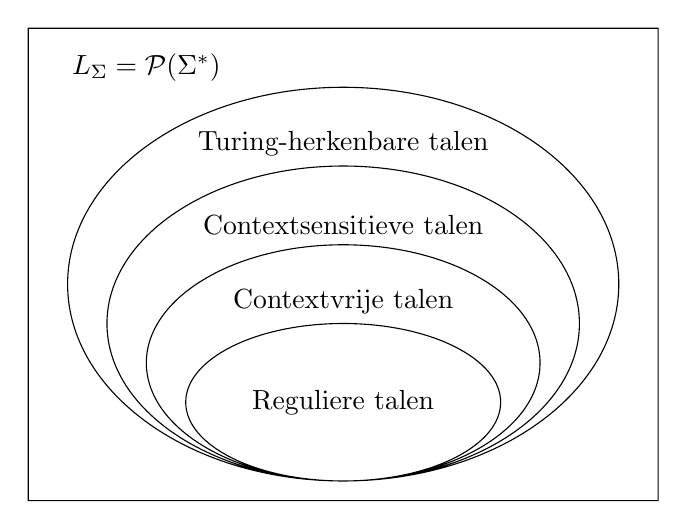
\begin{tikzpicture}
  \path
    (0,0) rectangle (8,6) [draw]
    (1.5,5.5) node {$L_\Sigma = \powerset(\sstar)$}
    (4,2.75) coordinate (A) node[above=1.5cm] {Turing-herkenbare talen} ellipse (3.5 and 2.5) [draw]
    (4,2.25) coordinate (B) node[above=1cm] {Contextsensitieve talen} ellipse (3 and 2) [draw]
    (4,1.75) coordinate (C) node[above=0.5cm] {Contextvrije talen} ellipse (2.5 and 1.5) [draw]
    (4,1.25) coordinate (D) node {Reguliere talen} ellipse (2 and 1) [draw];
\end{tikzpicture}
\end{center}

\textit{Zijn de talen van een TM beslisbaar?}

De verzameling van de talen die bepaald worden door een Turingmachine, of m.a.w. Turing-herkenbaar zijn is niet beslisbaar. Dit is equivalent met de vraag, kunnen we voor elke string $s \in L$ waarbij $L$ een taal is die door een machine $TM$ herkent wordt, beslissen dat $s$ door $TM$ geaccepteerd wordt? Dat is het acceptatieprobleem, wat niet beslisbaar is.

\subsection{Turingmachines}

\subsubsection{Vraag 1 - $\atm$}

\textit{Bewijs in detail dat $\atm$ niet beslisbaar is - steun daarbij niet op de stelling van Rice.}

We bewijzen dit door contradictie. Stel dat er een beslisser $B$ bestaat voor $\atm$. Bij een input $\langle M,s \rangle$ accepteert $B$ $M$ als $M$ $s$ accepteert en $B$ verwerpt $M$ als $M$ $S$ verwerpt of blijft lopen.

We construeren nu een contradictiemachine $C$ als
\begin{equation*}
C(\langle M \rangle) = opposite(B(\langle M,M \rangle))\text{ voor elke Turingmachine M}
\end{equation*}
De functie $opposite(x)$ is gedefinieerd als
\begin{equation*}
opposite(x) = \begin{cases}
reject, & \text{ als } x = accept\\
accept & \text{ als } x = reject
\end{cases}
\end{equation*}

We nemen nu $C(\langle C \rangle) = opposite(B(\langle C,C \rangle))$:
Als $C(\langle C \rangle) = accept$ ($C$ accepteert $C$), dan accepteert de beslisser $B$ de invoer $\langle C,C \rangle$, dus $B(\langle C,C \rangle) = accept$. Maar $opposite(B(\langle C,C \rangle))$ is dan $reject$, dat is een tegenstelling omdat dan geldt $C(\langle C \rangle) \neq opposite(B(\langle C,C \rangle))$.

We kunnen nu zeggen dat de machine $C$ niet kan bestaan, dus de beslisser $B$ kan ook niet bestaan. Bij gevolg is $\atm$ niet beslisbaar.

\textit{Zou het helpen als het toegelaten was op de stelling van Rice te steunen?}

Nee. We hebben de stelling van Rice bewezen door $\atm$ te reduceren naar $Pos_P$, om aan te tonen dat $Pos_P$ niet beslisbaar is omdat $\atm$ niet beslisbaar is. Met andere woorden, het bewijs voor de stelling van Rice steunt op het bewijs dat $\atm$ niet beslisbaar is en dus kan de stelling niet gebruikt worden om dat te bewijzen.

\textit{Is $\atm$ herkenbaar?}

Ja, $\atm$ is herkenbaar. We kunnen namelijk een enumerator machine bouwen dit $\atm$ herkent.

\textit{Is $\atm$ co-herkenbaar?}

Nee, indien het co-herkenbaar was, zou het ook beslisbaar moeten zijn omdat het herkenbaar is.

\subsubsection{Vraag 2 - $\etm$}

\textit{Geef het bewijs van de stelling $\etm$ is niet beslisbaar: doe dat zonder de stelling van Rice te gebruiken.}

  Stel dat $\etm$ beslisbaar is en $E$ is een beslisser voor $\etm$, dan kunnen we een beslisser $B$ voor $\atm$ construeren. Voor een gegeven invoer $\langle M,s \rangle$ construeren we een machine $M_s$ waarvoor geldt
  \begin{itemize}
  \item Gegeven een invoer $w$, als $w \neq s$, verwerpt $M_s$ de string $w$.
  \item Anders laat $M_s$ $M$ lopen op $w$ en geeft hetzelfde resultaat terug.
  \end{itemize}
  $M_s$ is een machine die enkel accept teruggeeft indien $M$ $s$ accepteert en anders reject. We laten $E$ lopen op $\langle M_s \rangle$:
  \begin{itemize}
  \item Als $E$ $M_s$ accepteert, dan laten we $B$ zijn input $\langle M,s \rangle$ verwerpen, omdat $M_s$ dan de lege taal bepaalt, wat enkel mogelijk is als $M$ $s$ verwerpt.
  \item Als $E$ $M_s$ verwerpt, dan laten we $B$ zijn input $\langle M,s \rangle$ accepteren, omdat $M_s$ dan niet de lege taal bepaalt, wat enkel mogelijk is als $M$ $s$ accepteert.
  \end{itemize}

\textit{Bespreek daarna de uitspraken $\etm$ is herkenbaar en $\etm$ is co-herkenbaar.}

Indien het herkenbaar was, zou het ook beslisbaar moeten zijn omdat het co-herkenbaar is.

$\etm$ is co-herkenbaar. We kunnen namelijk een enumerator machine bouwen dit $\overline{\etm}$ herkent.

\textit{Ken je ook alternatieve bewijzen?}

We kunnen dit bewijzen met de stelling van Rice. Bovendien is het ook mogelijk om aan te tonen dat $\etm$ beslisbaar is t.o.v. $\atm$ ($\etm \leq_T \atm$) met een orakel voor $\atm$:

  We construeren een Orakelmachine $\oatm$. Bij input $\langle M \rangle$ doet $\oatm$:
  \begin{itemize}
  \item Construeer een Turingmachine $P$ die bij input $w$:
  \begin{itemize}
  \item $M$ laat lopen op alle strings van $\sstar$.
  \item Als $M$ eender welke string van $\sstar$ accepteert, dan accepteert $P$ de input $w$. ($P$ accepteert voor eendere welke $w$ zo lang dat $M$ minstens \'e\'en string accepteert en dus niet de lege taal bepaalt.)
  \end{itemize}
  \item $\oatm$ vraagt aan het orakel of $\langle P,w \rangle \in \atm$.
  \item Als het orakel ``ja'' antwoordt, dan verwerpt $\oatm$ de invoer, omdat $M$ niet de lege taal bepaalt. Anders accepteert het de invoer.
  \end{itemize}
  
  $\oatm$ is een beslisser voor de taal $\etm$.

\textit{Hoe zit het met $E_{CFG}$?}

  We kunnen bewijzen dat $E_{CFG} = \{\langle G \rangle | G \text{ is een CFG en } L_G = \emptyset\}$ beslisbaar is door $G$ te transformeren als volgt:
  \begin{itemize}
  \item Voor een regel $A \rightarrow \alpha$ met $\alpha$ bestaande enkel uit terminals (inclusief $\epsilon$), dan:
  \begin{itemize}
  \item Verwijder alle producties waar $A$ aan de linkerkant staat.
  \item Vervang in elke regel waar $A$ rechts voorkomt, de voorkomens van $A$ door $\alpha$.
  \end{itemize}
  \item Herhaal de transformatie totdat:
  \begin{itemize}
  \item Het startsymbool verwijderd is, waarbij de invoer verworpen wordt, omdat dat betekent dat het mogelijk is een string af te leiden in het startsymbool.
  \item Er geen regels zijn van de benodigde vorm, waarbij de invoer aanvaard wordt, omdat de taal dan leeg is. (Het is dus niet mogelijk om een terminal te bereiken vanuit het startsymbool.)
  \end{itemize}
  \end{itemize}
  Door deze transformatie uit te voeren kunnen we voor elke CFG bepalen of die de lege taal bepaalt of niet en dus is $E_{CFG}$ beslisbaar.
  
  Merk op dat de grammatica getransformeerd wordt naar een niet-equivalente grammatica.

\subsubsection{Vraag 3 - Enumerator machine}

\textit{Definieer de enumerator machine.}

Een enumeratormachine is een variant van een Turingmachine (definitie \ref{def:tm}) met een extra enumeratortoestand $q_e$ en een overgangsfunctie met als signatuur \bm{$\delta: Q \times \Gamma \rightarrow Q \times \Gamma \times \Gamma_\epsilon \times \{L, R, S\}$}. Bij een overgang wordt voor $\Gamma_\epsilon$ in de signatuur een teken op een outputband geschreven. Bij het bereiken van $q_e$ wordt een outputmarker op de outputband geschreven die een outputstring afscheidt van de volgende.

\textit{Bewijs dat elke herkenbare taal kan ge\"enumereerd worden en dat elke taal die door een enumerator wordt ge\"enumereerd ook herkenbaar is.}

\paragraph{Elke herkenbare taal kan ge\"enumereerd worden.}
  Het Halting-probleem geeft aan dat een Turingmachine niet noodzakelijk stopt voor elke string. Daarom construeren we een enumerator $Enu$ voor een herkenbare taal $L$ bepaald door $TM$ als volgt:
 
  We construeren
  \begin{itemize}
  \item een Turingmachine $TM_{gen}$ die gegeven een getal $n$, de $n$ eerste strings van $\sstar$ op de band zet.
  \item een Turingmachine $TM_n$ die gegeven een getal $N$, op elk van de $n$ strings, $n$ stappen van $TM$ uitvoert. Als $TM$ daarbij een string accepteert, dan wordt die weggeschreven op de outputband van $Enu$.
  \item een Turingmachine $TM_{driver}$ die opeenvolgende getallen $n$ genereert en vervolgens $TM_{gen}$ en $TM_n$ oproept.
  \end{itemize}

\paragraph{Elke taal die door een enumerator wordt ge\"enumereerd is herkenbaar.}
We construeren een herkenner $H$ voor de taal $L$ bepaald door een gegeven enumerator $Enu$. Bij de invoer van een string $s \in L$ laat $H$ $Enu$ lopen. Telkens $Enu$ de toestand $q_e$ bereikt, vergelijkt $H$ de gegeven string $s$ met de laatste string op de outputband. Als ze gelijk zijn, dan accepteert $H$ de taal, als ze niet gelijk zijn, laat het $Enu$ de volgende string genereren.

\textit{Kan elke beslisbare taal ge\"enumereerd worden?}

Elke beslisbare taal is ook een herkenbare taal. Omdat elke herkenbare taal ge\"enumereerd kan worden kan ook elke beslisbare taal ge\"enumereerd worden.

\textit{Bespreek in deze context de uitspraak ``de verzameling van Turingmachines is een herkenbare taal''.}

Elke Turingmachine herkent een taal en elke herkenbare taal is enumereerbaar, dus moet ook de verzameling van alle Turingmachines enumereerbaar en dus herkenbaar zijn.

\subsubsection{Vraag 4 - Stelling van Rice}

\textit{Leg de stelling van Rice uit, en geef het bewijs.}

  Voor elke niet-triviale, taal-invariante eigenschap $P$ van Turingmachines geldt dat $Pos_P$ niet beslisbaar is. (Ook $Neg_P$ is niet beslisbaar, maar dat volgt uit $Neg_P = \overline{Pos_P}$.)

\paragraph{Bewijs.}   Stel dat $M_\emptyset$ die de lege taal bepaalt, een eigenschap $P$ niet heeft. Omdat $P$ niet-triviaal is, moet er een machine $X$ bestaat die de taal $L_X$ bepaalt en de eigenschap $P$ wel heeft.

  Stel dat er een beslisser $B$ bestaan voor $Pos_P$, dan kunnen we een beslisser $A$ voor $A_{TM}$ construeren. Voor een gegeven invoer $\langle M,s \rangle$ construeren we een hulpmachine $H_{M,s}$ waarvoor geldt
  \begin{itemize}
  \item $H_{M,s}$ laat $M$ lopen op $s$.
  \item Als $M$ $s$ accepteert, dan laat $H_{M,s}$ $X$ lopen op een invoer $x$ en accepteert indien $X$ $x$ accepteert.
  \end{itemize}
  
  We kunnen zeggen dat voor $H_{M,s}$ geldt dat het de taal $L_X$ bepaalt indien $M$ $s$ accepteert en de lege taal bepaalt indien $M$ $s$ niet accepteert. Dat wilt zeggen dat $H_{M,s}$ de eigenschap $P$ heeft indien $M$ $s$ accepteert en de eigenschap $P$ niet heeft indien $M$ $s$ niet accepteert.
  
  Bijgevolg kunnen we zeggen dat $A$ een invoer $\langle M,s \rangle$ accepteert als $B$ $H_{M,s}$ accepteert en de invoer verwerpt als $B$ $H_{M,s}$ verwerpt. Dus $A$ is een beslisser voor $\atm$, wat niet mogelijk is. Daarom kan de beslisser $B$ voor $Pos_P$ ook niet bestaan.
  
  We zeggen dat $\atm$ reduceerbaar is naar $Pos_P$.
  
  Als $M_\emptyset$ de eigenschap $P$ wel heeft, kunnen we het bewijs uitvoeren voor $\overline{P}$. Omdat we dan bewijzen dat $Pos_{\overline{P}} = Neg_P$ onbeslisbaar is, weten we dat ook $Pos_P = \overline{Neg_P}$ onbeslisbaar is.

\textit{Geef minstens \'e\'en eigenschap van Turingmachines die niet voldoet aan de voorwaarde voor de stelling van Rice, en laat zien dat die eigenschap geen aanleiding geeft tot een niet-beslisbare taal.}

De eigenschap ``de taal bepaald door een Turingmachine moet herkenbaar zijn'' is triviaal, omdat elke Turingmachine een Turing-herkenbare taal bepaalt. Dus deze eigenschap voldoet niet aan de stelling van Rice.

Indien deze eigenschap aanleiding zou geven tot een niet-beslisbare taal, dan zou elke herkenbare taal niet-beslisbaar moeten zijn. We weten echter dat elke beslisbare taal ook herkenbaar is.

\subsubsection{Vraag 4 (Bijvraag 1)}

\textit{Karakteriseer volledig alle eigenschappen van Turingmachines die aan de stelling van Rice voldoen m.b.v. $IsIn_{TM,S}$.}

$IsIn_{TM,S}$ is de verzameling van alle Turingmachines $M$ die een taal $L_M$ bepalen die deel uitmaakt van de verzameling $S$. We zoeken een eigenschap $P$ van een Turingmachine $M$ zodanig dat
\begin{equation*}
  L_M \in S \leftrightarrow M \in Pos_P \en M \notin Neg_P
\end{equation*} 

Indien de eigenschap $P$ aan de stelling van Rice voldoet, is $IsIn_{TM,S}$ niet beslisbaar, want dan geldt $IsIn_{TM,S} = Pos_P$.

\subsubsection{Vraag 5 - Orakelmachine}

\textit{Wat is een orakelmachine?}

Een orakelmachine is een Turingmachine die een orakel kan raadplegen om de oplossing voor een bepaald probleem te vragen.

Aan een orakel voor $\atm$ kan een TM bijvoorbeeld vragen of een machine $M$ een string $s$ accepteert.

\textit{Bespreek de uitspraak: "de verzameling orakelmachines (over een gegeven orakel) is strikt krachtiger dan de verzameling van Turing machines". Leg hierbij ook uit wat je bedoelt met "krachtiger".}

Een verzameling $A$ is krachtiger (of sterker) dan een verzameling $B$ indien $B$ een deelverzameling is van $A$.

De verzameling van orakelmachines over een gegeven orakel is krachtiger dan de verzameling van de Turingmachines, omdat een orakelmachine een Turingmachine is, dus voor elke Turingmachine bestaat een equivalente orakelmachine die het orakel niet raadpleegt. Bovendien kan een orakelmachine problemen beslissen die een Turingmachine niet kan beslissen, wat maakt dat de verzameling van orakelmachines groter is dan de verzameling van Turingmachines en dus krachtiger.

Een voorbeeld is de orakelmachine $\oatm$ met een orakel voor $\atm$, die in staat is om $\atm$ te beslissen en bij gevolg ook heel wat andere problemen.

\textit{Kan een verzameling orakelmachines (voor bepaald gegeven orakel) alle talen beslissen?}

Nee, de verzameling van orakelmachines is (oneindig) aftelbaar, maar de verzameling van alle talen $L_\Sigma$ is niet-aftelbaar. Daarom moet er minstens \'e\'n taal zijn die een orakelmachine voor een bepaald orakel niet kan beslissen.

\subsubsection{Vraag 5 (Bijvraag 1)}

\textit{Kan een orakelmachine voor $\atm$, $\htm$ beslissen?}

Ja, je kan een orakelmachine $\oatm$ construeren die voor een input $\langle M,s \rangle$ beslist of die machine stopt voor de string $s$. Dat gebeurt als volgt:

\begin{itemize}
\item De machine vraagt aan het orakel of $M$ $s$ accepteert. Indien het antwoord ``ja'' is, dan accepteert $\oatm$ de invoer.
\item Anders construeren we een machine $M_i$ die gelijk is een $M$ met de uitzondering dat de accepterende en verwerpende toestanden gewisseld zijn. De machine vraagt aan het orakel of $M_i$ $s$ accepteert. Indien het antwoord ``ja'' is, dan accepteert $\oatm$ de invoer.
\item Anders verwerpt $\oatm$ de invoer, omdat we dan weten dat $M$ niet zal stoppen.
\end{itemize}

We kunnen zeggen dat $\htm \leq_T \atm$. Bovendien, omdat we weten dat $\atm \leq_m \htm$ en dus ook $\atm \leq_T \htm$, zeggen we dat $\atm \equiv_T \htm$ ($\atm$ en $\htm$ zijn Turing-equivalent).

\subsubsection{Vraag 6 - Reduceerbaarheid}

\textit{Bespreek de twee noties van reduceerbaarheid ($A \leq_m B$ en $A \leq_T B$), hun verband en op welke manier die noties kunnen gebruikt worden om aan te tonen dat een taal (on)beslisbaar/herkenbaar is.}

\paragraph{Reduceerbaarheid.} Een taal $L_1$ over $\Sigma_1$ kan gereduceerd worden naar een taal $L_2$ over $\Sigma_2$ als er een afbeelding \bm{$f: \sstar_1 \rightarrow \sstar_2$} bestaat zodanig dat $f(L_1) \subseteq L_2$ en $f(\overline{L_1}) \subseteq \overline{L_2}$ met $f$ een Turing-berkenbare functie.

Indien een taal $A$ niet-beslisbaar is en reduceerbaar is naar een andere taal $B$, dan moet $B$ ook niet-beslisbaar zijn. Omdat we anders de beslisser van $B$ zouden kunnen gebruiken om $A$ te beslissen. We zeggen dus ook dat $A$ beslisbaar is als $B$ beslisbaar is. Dit geldt analoog voor herkenbaarheid.

\paragraph{Turingreduceerbaarheid.} Een taal $A$ is Turingeduceerbaar naar een taal $B$ indien er een orakelmachine $O^B$ bestaat die $A$ beslist. We zeggen dat $A$ beslisbaar is t.o.v. $B$.

Indien een taal $B$ beslisbaar is en een taal $A$ Turingreduceerbaar is naar $B$, dan moet $A$ ook beslisbaar zijn.

\paragraph{Verband.} Turingreduceerbaarheid is fijner dan reduceerbaarheid. Elk probleem $A$ dat reduceerbaar is naar $B$ moet ook Turingreduceerbaar zijn naar $B$.

\subsection{Lambda calculus}

\subsubsection{Vraag 1 - Church-Rosser}

\textit{Formuleer en bespreek de stellingen van Church-Rosser.}

\paragraph{CR1.}   Church-Rosser I verwijst naar de eerste stelling van Church en Rosser. Die stelling zegt dat indien $E_1 \stackrel{*}{\longleftrightarrow} E_2$ geldt, dat er een expressie $E$ moet bestaan in normaalvorm zodanig dat $E_1 \stackrel{*}{\longrightarrow} E$ en $E_2 \stackrel{*}{\longrightarrow} E$.

Uit de eerste stelling volgt de uniciteit van de normaalvorm. Dat wilt zeggen dat de normaalvorm van een expressie altijd uniek is en enkel kan verschillen onder $\alpha$-reductie.

\paragraph{CR2.}   Church-Rosser II verwijst naar de tweede stelling van Church en Rosser. Die stelling zegt dat indien $E \stackrel{*}{\longleftrightarrow} N$  bestaat met $N$ in normaalvorm, dat er een reductierij moet bestaan in normaalorde van $E$ naar $N$.

\textit{Geef daarbij hun belang i.v.m. het baseren van een programmeertaal op lambda-calculus.}

De eerste stelling is belangrijk omdat het in essentie zegt dat het reduceren van een lambda-expressie altijd hetzelfde resultaat zal produceren.

De tweede stelling is belangrijk omdat de reductie in normaalorde zorgt voor ``lazy evaluation''. Een techniek waarbij een expressie enkel wordt ge\"evalueerd indien de waarde van die expressie nodig is. Een voorbeeld daarvan is het evalueren van een ``OR'' expressie. Het tweede argument van die expressie zal enkel ge\"evalueerd worden indien het eerste argument naar ``FALSE'' evalueert, omdat anders het resultaat van de expressie reeds ``TRUE'' zal zijn.

\textit{Geef de relatie met de programmeertaal Haskell.}

$\lambda$-calculus vormt de basis van de klasse van functionele programmeertalen. Haskell is een voorbeeld van een functionele programmeertaal, vernoemd naar de wiskunde Haskell Curry, wiens achternaam ook gebruik wordt voor de techniek ``currying'' bij functionele (en logische) programmeertalen en wie ook \'e\'en van de meest gekende vastpuntcombinators heeft bedacht.

\subsubsection{Vraag 1 (Bijvraag 1)}

\textit{Is $\lambda$-calculus Turing-compleet?}

Ja, het is mogelijk om elke (universele) Turingmachine in $\lambda$-calculus voor te stellen, omdat het elke Turing-berkenbare functie kan voorstellen.

\subsubsection{Vraag 1 (Bijvraag 2)}

\textit{Hoeveel conversieregels ken je?}

Er zijn drie conversieregels, namelijk:

\begin{itemize}
\item $\alpha$-conversie: Het hernoemen van variabelen.
\item $\beta$-conversie: Functie evaluatie.
\item $\eta$-conversie: Equivalentie onder redundante $\lambda$-abstracties.
\end{itemize}

Een vierde conversieregel, $\delta$-conversie wordt meestal niet vermeld. Dat is de evaluatie van ingebouwde functies.

\subsubsection{Vraag 1 (Bijvraag 3)}

\textit{Laat daarna zien hoe je in zuivere lambda-calculus recursieve functies kan defini\"eren. Doe dat m.b.v. een voorbeeld recursieve functie verschillend van FAC uit de cursus.}

Het is mogelijk om in $\lambda$-calculus een recursieve functie gebruik te maken van een vastpuntcombinator. Dat is een zelf-replicerende expressie. De meest voorkomende vastpuntcombinator werd voorgesteld door Haskell Curry:
\begin{equation*}
  Y\ F = F\ (Y\ F) \text{ met } Y = \lambda f.\ (\lambda x.\ f\ (x\ x))\ (\lambda x.\ f\ (x\ x))
\end{equation*}

Stel dat een $\lambda$-calculus niet beschikt over een optel functie, maar wel over een functie $INC$ om een getal met \'e\'en te verhogen en $DEC$ om dat getal met \'e\'en te verlagen. We stellen een recursieve functie $PLUS$ op, die een getal bij een ander getal optelt.

\begin{equation*}
  H = \lambda f,a,b.\ (IF\ (=\ b\ 0)\ a\ (f\ (INC\ a)\ (DEC\ b))) \text{ met } PLUS = H\ PLUS
\end{equation*}

$H$ is het vastpunt voor $PLUS$, nu kunnen we de defini\"erende vergelijking $PLUS = H\ PLUS$ vervangen met de vastpuntcombinator, zodat we $PLUS = Y H$ bekomen.

We kunnen nu een bewerking met deze functie uitvoeren:

\begin{equation*}
\begin{aligned}
PLUS\ 4\ 1 = \\
Y\ H\ 4\ 1 = \\
H\ (Y\ H)\ 4\ 1 = \\
\lambda f,a,b.\ (IF\ (=\ b\ 0)\ a\ (f\ (INC\ a)\ (DEC\ b)))\ (Y\ H)\ 4\ 1 \longrightarrow \\
\lambda a,b.\ (IF\ (=\ b\ 0)\ a\ ((Y\ H)\ (INC\ a)\ (DEC\ b)))\ 4\ 1 \stackrel{*}{\longrightarrow} \\
(IF\ (=\ 1\ 0)\ 4\ ((Y\ H)\ (INC\ 4)\ (DEC\ 1))) \longrightarrow \\
(IF\ FALSE\ 4\ ((Y\ H)\ (INC\ 4)\ (DEC\ 1))) \longrightarrow \\
(Y\ H)\ (INC\ 4)\ (DEC\ 1) \stackrel{*}{\longrightarrow} \\
(Y\ H)\ 5\ 0 = \\
\lambda f,a,b.\ (IF\ (=\ b\ 0)\ a\ (f\ (INC\ a)\ (DEC\ b)))\ (Y\ H)\ 5\ 0 \longrightarrow \\
\lambda a,b.\ (IF\ (=\ b\ 0)\ a\ ((Y\ H)\ (INC\ a)\ (DEC\ b)))\ 5\ 0 \stackrel{*}{\longrightarrow} \\
(IF\ (=\ 0\ 0)\ 5\ ((Y\ H)\ (INC\ 5)\ (DEC\ 0))) \longrightarrow \\
(IF\ TRUE\ 5\ ((Y\ H)\ (INC\ 5)\ (DEC\ 0))) \longrightarrow \\
5
\end{aligned}
\end{equation*}

\end{document}
